% This must be in the first 5 lines to tell arXiv to use pdfLaTeX, which is strongly recommended.
\pdfoutput=1
% In particular, the hyperref package requires pdfLaTeX in order to break URLs across lines.

\documentclass[11pt]{article}

% Remove the "review" option to generate the final version.
\usepackage[review]{naacl2021}

% Standard package includes
\usepackage{times}
\usepackage{latexsym}

% For proper rendering and hyphenation of words containing Latin characters (including in bib files)
\usepackage[T1]{fontenc}
% For Vietnamese characters
% \usepackage[T5]{fontenc}
% See https://www.latex-project.org/help/documentation/encguide.pdf for other character sets

% This assumes your files are encoded as UTF8
\usepackage[utf8]{inputenc}
%\usepackage[utf8x]{inputenc}

% This is not strictly necessary, and may be commented out,
% but it will improve the layout of the manuscript,
% and will typically save some space.
\usepackage{microtype}


% for jon edits
%\usepackage{setspace}
% \doublespacing




%\usepackage[UTF8]{ctex}
%\documentclass[UTF8]{ctexart}
%\usepackage{xeCJK}
%\setCJKmainfont{BabelStone Han}

%\usepackage{verbatim}
\usepackage{listings}

\usepackage{hyperref}
\usepackage{tablefootnote}

\usepackage{pifont}% http://ctan.org/pkg/pifont
\newcommand{\cmark}{\ding{51}}%
\newcommand{\xmark}{\ding{55}}%

\usepackage{amsmath}
\usepackage{verbatim}
\usepackage{textcomp} 
\usepackage{enumitem} 

\usepackage{multirow}
%\usepackage{arydshln}
\usepackage{caption}
\usepackage{subcaption}
%\usepackage{rotating} 
%\usepackage{float}


%\newcommand*\justify{%
%  \fontdimen2\font=0.4em% interword space
%  \fontdimen3\font=0.2em% interword stretch
%  \fontdimen4\font=0.1em% interword shrink
%  \fontdimen7\font=0.1em% extra space
%  \hyphenchar\font=`\-% allowing hyphenation
%}


%\usepackage{yhmath}


\newcommand{\bleu}{{\textsc{Bleu}}}
\newcommand{\chr}[2]{{C\small{HR}{#1}$_{{#2}}$}}
\newcommand{\chrx}[1]{\text{\small{CHR}\large{#1}}}

\newcommand{\chrf}[1]{\textsc{ChrF}{$_{#1}$}}
\newcommand{\bleufx}[1]{{B\small{LEU}F$_{{#1}}$}}
\newcommand{\bleuf}{{\textsc{BleuF}}}

\newcommand{\maf}[1]{\textsc{MacroF}{\text{$_{{#1}}$}}}
\newcommand{\mif}[1]{\textsc{MicroF}{\text{$_{{#1}}$}}}
\newcommand{\mableu}{\textsc{MacroBleu}}
\newcommand{\mibleu}{\textsc{MicroBleu}}
\newcommand{\blrtmn}{\textsc{BLEURT}\text{\footnotesize{}mean}}
\newcommand{\blrtmd}{\textsc{BLEURT}\text{\footnotesize{}median}}
%\newcommand{\blrtmn}{$\overline{\textsc{Bleurt}}$}
%\newcommand{\blrtmd}{$\widetilde{\textsc{Bleurt}}$}
%\newcommand{\blrtmd}{$\overbrace{\textsc{Bleurt}}$}


%\usepackage[dvipsnames]{xcolor} % already imported
\newcommand{\colorann}[3]{\textcolor{#1}{${}^{#2}[$#3$]$}}
%\newcommand{\jon}[1]{\colorann{red}{Jon}{\footnotesize #1}}
%\newcommand{\tg}[1]{\colorann{cyan}{TG}{\footnotesize #1}}
%\newcommand{\wy}[1]{\colorann{orange}{WY}{\footnotesize #1}}
%\newcommand{\cl}[1]{\colorann{green}{CL}{\footnotesize #1}}

%\newcommand{\argmin}{\operatornamewithlimits{argmin}}
%\newcommand{\argmax}{\operatornamewithlimits{argmax}}
\newcommand{\insig}{$^{\times}$}

\usepackage{amssymb}

%\newcommand{\myurl}[1]{\href{#1}{\small{#1}}}
\newcommand{\myurl}[1]{\href{#1}{#1}}

%\documentclass[tikz,border=4mm]{standalone}
\usepackage{tikz}
\usepackage[normalem]{ulem}
\usetikzlibrary{positioning,fit,calc,backgrounds}
\tikzset{block/.style={draw,thick,text width=2cm,minimum height=1cm,align=center},
         line/.style={-latex}
}
\makeatletter
\def\ruwave{\bgroup \markoverwith{\lower3.5\p@\hbox{\textcolor{red}{\sixly \char58}}}\ULon}
\font\sixly=lasy6
\makeatother



% Weiqiu
% not sure what to call it yet...
\usepackage{graphicx,wasysym}
%\usepackage{xspace,mfirstuc,tabulary}
\newcommand{\deleterious}[3]{{\Large\frownie{}}_{#1\to#2}^{#3}}
\newcommand{\beneficial}[3]{{\Large\smiley{}}_{#1\to#2}^{#3}}
\newcommand{\scoredel}[3]{\delta_{#3}^{#1^{#2}}}



\title{Macro-Average: Rare Types Are Important Too}
% maybe just limit to MacroF1
% maybe say "All Words are Important, But Rare Words Are Especially Important"

% Author information does not appear in the pdf unless the "acceptedWithA" option is given
% See tacl2018v2.sty for other ways to format author information
\author{
 Template Author\Thanks{The {\em actual} contributors to this instruction
 document and corresponding template file are given in Section
 \ref{sec:contributors}.} \\
 Template Affiliation/Address Line 1 \\
 Template Affiliation/Address Line 2 \\
 Template Affiliation/Address Line 2 \\
  {\sf template.email@sampledomain.com} \\
}

%% Authors: Thamme Gowda, Weiqiu You, Constantine Lignos, Jonathan May
%% Maybe some of them be moved to Acknowledgements
%%   Shantanu Agarwal, Joel Barry, Scott Miller,  Daniel Cohen ??, 

\date{}

\begin{document}
\maketitle
\begin{abstract}
  %Information theory and Zipf's law states that much of the information of a language system is in the long tail, however, the current metrics for natural language generation~(NLG) place only a little importance on the long tail. 

% JON: What does adequacy mean in general for NLG? That only really makes sense for MT unless you make a long argument. The NLG tests are mostly aimed at that so let's just stick with MT

%The  current  corpus-level  evaluation  metrics for  natural  language  generation  (NLG)  are good  in  capturing  the  fluency,  however,  fall short  in  capturing  adequacy.

%Recently, machine learning model-based metrics that are trained to predict quality at segment-level have attracted the attention due to their high performance on certain benchmark tasks. 
%However, the non-transparency, and biased nature of model-based evaluation are concerning for real-world applications.
% and achieves higher association with adequacy than others. 
%\maf1 is easily interpretable, free from data-induces biases.% \  higher importance to rare types from long tail.
%\wy{Did we define MacroF1 or just reexamine its use in generation?}
%and another that assigns higher importance to frequent types similar to current methods.  We compare them along with popular alternatives and show that our method that assigns higher importance to the Long Tail is very useful.
%We justify its utility in the direct evaluation of NLG systems as well as indirect evaluation on downstream tasks.
%and has the capacity to discriminate between structurally different machine translation methods in a way other methods cannot. 

While traditional corpus-level evaluation metrics for machine translation correlate well with fluency, they struggle to reflect adequacy.
Model-based MT metrics trained on segment-level human judgments have emerged as an attractive replacement due to strong correlation results.
These models, however, require potentially expensive re-training for new domains and languages.
Furthermore, their decisions are inherently non-transparent and appear to reflect unwelcome biases. 
We explore the simple type-based classifier metric, \maf1, and study its applicability to MT evaluation. 
We find that \maf1 is competitive on direct assessment, and outperforms others in indicating downstream cross-lingual information retrieval task performance.
Further, we show that \maf1 can be used to effectively compare supervised and unsupervised neural machine translation, and reveal significant qualitative differences in the methods' outputs.\footnote{Tools and analysis are available at \myurl{https://github.com/HELD-FOR-ANONYMITY}
}

%\myurl{https://github.com/thammegowda/007-mt-eval-macro}

\end{abstract}



\section{Introduction}

Model-based metrics for evaluating machine translation such as BLEURT \cite{sellam-etal-2020-bleurt}, ESIM \cite{mathur-etal-2019-ESIM}, and YiSi \cite{lo-2019-yisi} have recently attracted attention due to their superior correlation with human judgments \cite{WMT19-metrics-proceedings}. However, \bleu~\cite{papineni-etal-2002-bleu} remains  the most widely used corpus-level MT metric. It correlates reasonably well with human judgments, and moreover is easy to understand and cheap to calculate, requiring only reference translations in the target language. By contrast, model-based metrics require tuning on thousands of examples of human evaluation for every new target language or domain \cite{sellam-etal-2020-bleurt}. Model-based metric scores are also opaque and can hide undesirable biases, as can be seen in Table~\ref{tab:bleurt-bias}.


\begin{table}[ht]
    \centering
    \footnotesize
    \begin{tabular}{l l l }
Reference:& \multicolumn{2}{l}{You must be a doctor.} \\
Hypothesis: & \multicolumn{2}{l}{$\rule{1cm}{0.15mm}$ must be a doctor.} \\
    % & You &	~0.990 \\
    & He	&-0.735 \\
    %& Alexandra & -0.888 \\
    %& Alexander & -0.975 \\
    & Joe & -0.975 \\
    & Sue & -1.043 \\
    & She	 &-1.100 \\\hline
Reference:& \multicolumn{2}{l}{It is the greatest country in the world.} \\
Hypothesis:& \multicolumn{2}{l}{$\rule{1cm}{0.15mm}$ is the greatest country in the world.} \\
    % & It	& ~0.957 \\
    & France &	-0.022 \\
    & America	& -0.060 \\
    & Russia &	-0.161 \\
    %& China  & -0.166 \\
    %& USA    & -0.168 \\
    %& India   &	-0.211 \\
    & Canada  & -0.309 
    \end{tabular}
    \caption{A demonstration of BLEURT's internal biases; model-free metrics like BLEU would consider each of the errors above to be equally wrong.}
    \label{tab:bleurt-bias}
\end{table}

The source of model-based metrics' (e.g. BLEURT) correlative superiority over model-free metrics (e.g. BLEU) appears to be the former's ability to focus evaluation on \textit{adequacy}, while the latter are overly focused on \textit{fluency}. BLEU and most other generation metrics consider each output \textit{token} equally. Since natural language is dominated by a few high-count types, an MT model that concentrates on getting its \textit{if}s, \textit{and}s and \textit{but}s right will benefit from BLEU in the long run more than one that gets its \textit{xylophone}s, \textit{peripatetic}s, and \textit{defenestrate}s right. Can we derive a metric with the discriminating power of BLEURT that does not share its bias or expense and is as interpretable as BLEU? 

As it turns out, the metric may already exist and be in common use. Information extraction and other areas concerned with classification have long used both \textit{micro averaging}, which treats each token equally, and \textit{macro averaging}, which instead treats each \textit{type} equally, when evaluating. The latter in particular is useful when seeking to avoid results dominated by overly frequent types.  In this work we take a classification-based approach to evaluating machine translation in order to obtain an easy-to-calculate metric that focuses on adequacy as much as BLEURT but does not have the expensive overhead, opacity, or bias of model-based methods. 


% \begin{figure}[ht!]
%     \centering
%     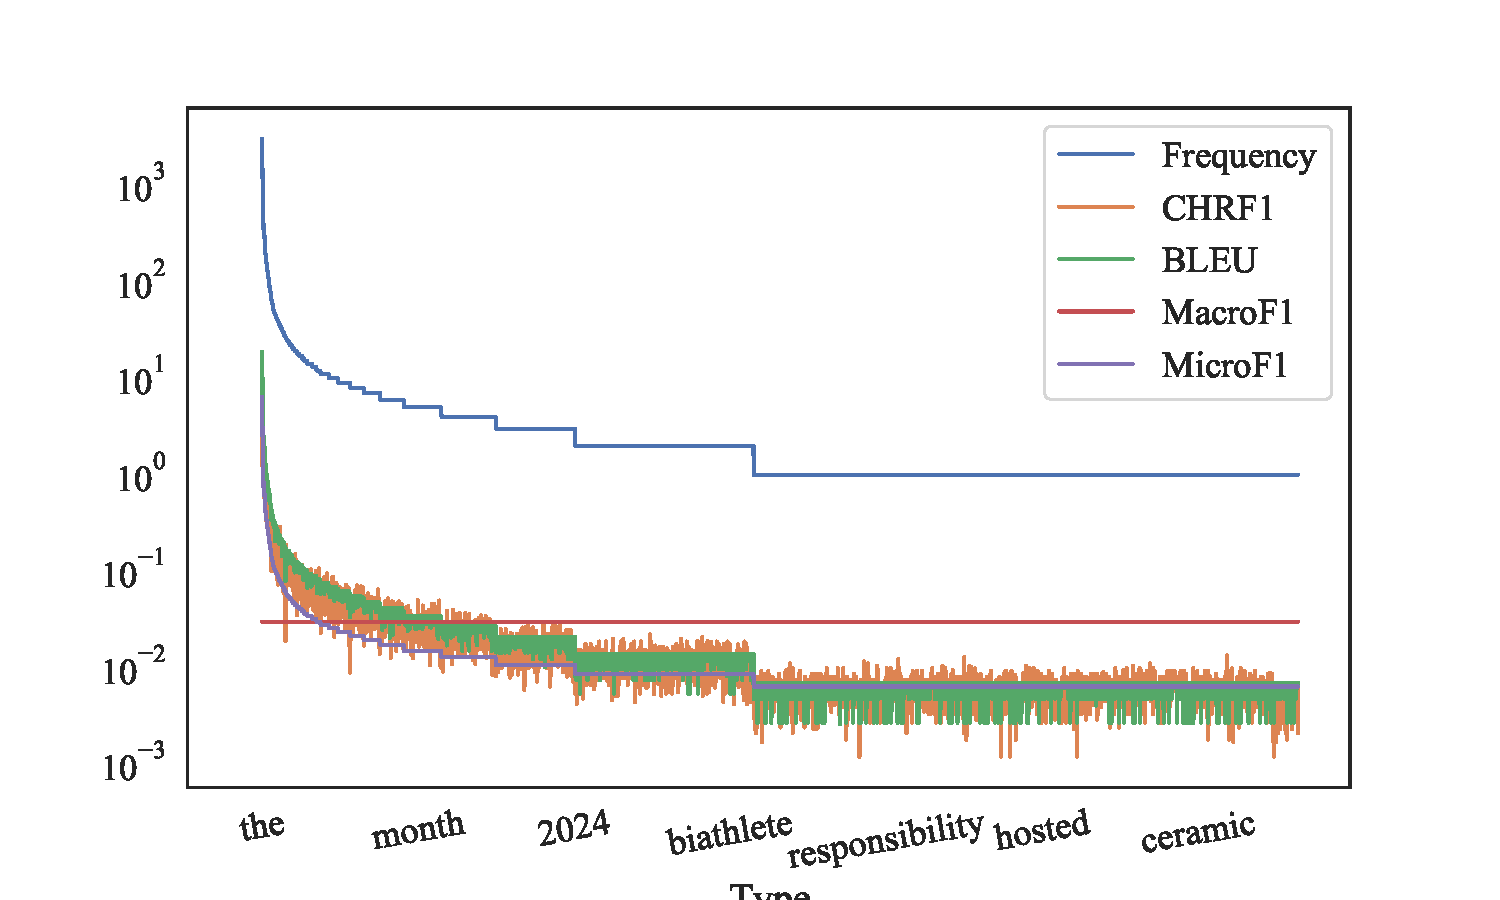
\includegraphics[width=\linewidth,trim={15mm 5mm 25mm 15mm},clip]{img/bleu-chrf-macro-micro-swapin-lenmatch.pdf}
%     %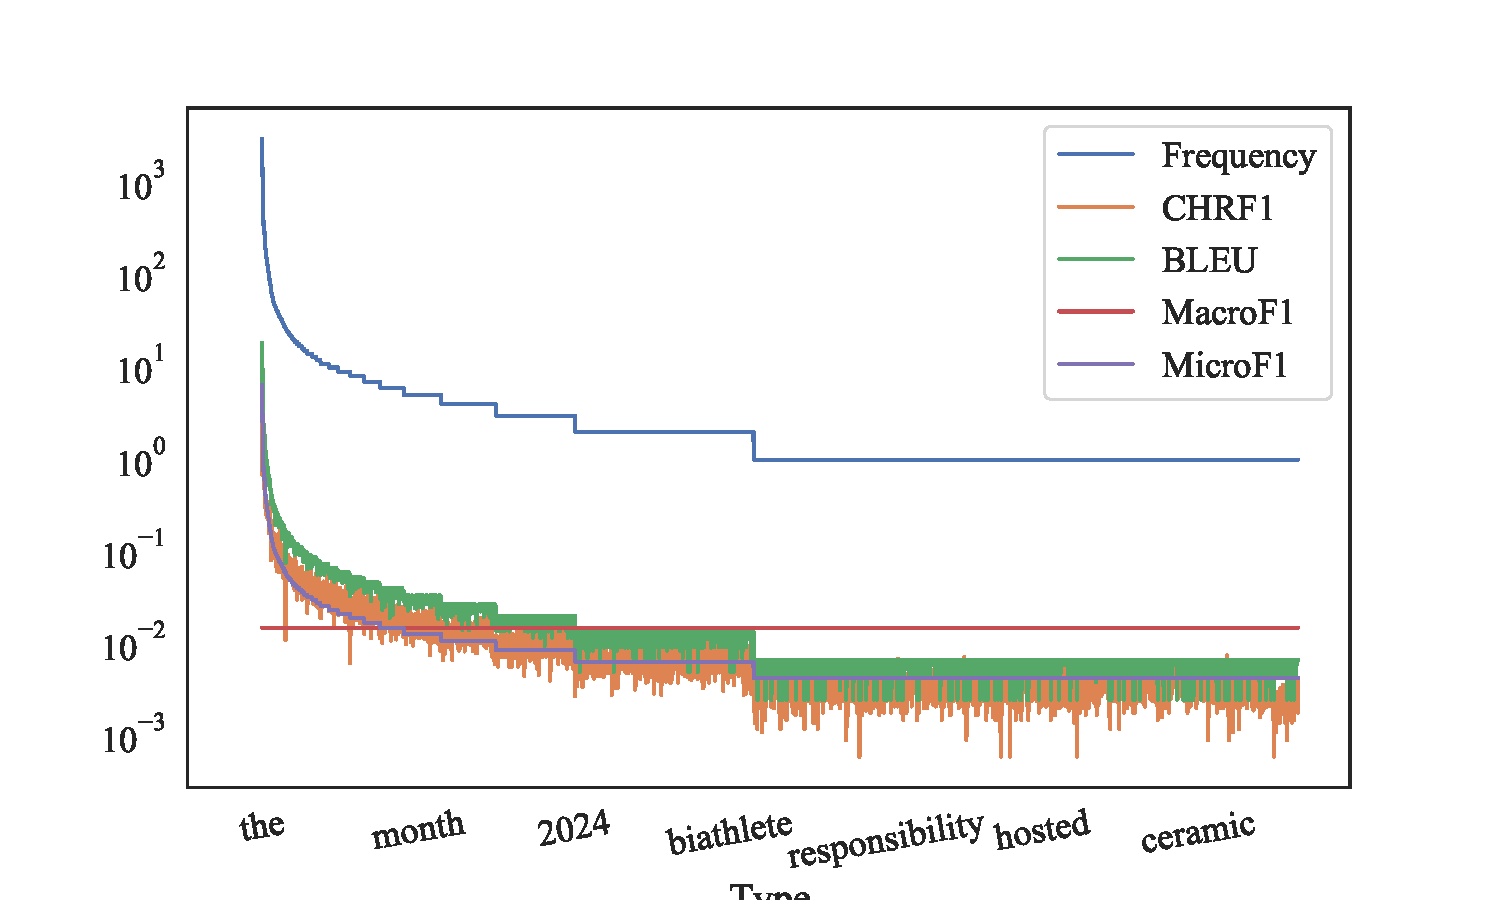
\includegraphics[width=\linewidth,trim={15mm 5mm 25mm 15mm},clip]{img/bleu-chrf-macro-micro-norecall.pdf}
%     \caption{\small Individual word type contribution to the corpus-level MT autoeval methods. % as measured on WMT NewsTest2019 German-English reference corpus.
%     The horizontal axis contains word types ranked by frequencies.
%     The vertical axis, which is in logarithmic scale, represents type frequencies (raw count) and percentile of contribution to the total corpus-level score. 
%     The contribution of a type is defined as the difference in corpus-level score between when the type is perfectly learned versus when it is fully ignored~(i.e zero-recall). 
%     %Perfect translations are simply when reference is treated as hypothesis where are as the full-ignorance or zero-recall is simulated for each type by replacing an out-of-vocabulary token of similar character count in the perfectly translated hypothesis~(therefore, no effect on length penalty).
%     %The roughness in lines of \bleu\ is and \chrf1 is due to the variation in n-grams affected by a type.
%     \mif1 uses only unigrams and scales the contribution by its frequency, whereas
%     \maf1, which is the focus of this work, is unweighted and assigns equal importance to all the types regardless of their frequencies. 
%     It is evident that the type contribution in \bleu\ and \chrf1 is scaled according to their frequency in the similar manner as \mif1.
%     For instance, `the' type appears 3019 times in the chosen test set, and zero-recall of `the' can result in loss up to 18.83\%, 9.38\%, 6.45\%, and 0.03\% of overall score in \bleu, \chrf1, \mif1, \maf1, respectively on the corpus used.
%     %Take away: \maf1 underscores the types on Long Tail where as others assign greater importance to the frequent words.
%     %Both \maf1 and \mif1 are described in detail in Section~\ref{sec:mt-cls-eval}.
%     }
% \label{fig:bleu-damage}
% \end{figure}



Our contributions are as follows:
We consider MT as a classification task, and thus admit \maf1 as a legitimate approach to evaluation~(Section ~\ref{sec:mt-as-cls}). 
We show that \maf1 is competitive with other popular methods at tracking human judgments in translation (Section~\ref{sec:wmt-metrics}). 
We offer an additional justification of \maf1 as a performance indicator on adequacy-focused downstream tasks such as cross-lingual information retrieval (Section \ref{sec:clir}). 
Finally, we demonstrate that \maf1 is just as good as the expensive BLEURT at discriminating between structurally different MT approaches in a way \bleu\ cannot, especially regarding the adequacy of generated text, and provide a novel approach to qualitative analysis of the effect of metrics choice on quantitative evaluation (Section \ref{sec:unmt}).



\section{NMT as Classification}
\label{sec:mt-as-cls}
Neural machine translation (NMT) models are often viewed as pairs of encoder-decoder networks.
Viewing NMT as such is useful in practice for implementation; however, such a view is inadequate for theoretical analysis. % of strengths and weaknesses of architecture.
\citet{gowda2020finding} provide a high-level view of NMT as two fundamental ML components: an autoregressor and a classifier. 
Specifically, NMT is viewed as a multi-class classifier that operates on representations from an autoregressor.
We may thus consider classifier-based evaluation metrics.


Consider a test corpus, $T = \{ (x^{(i)}, h^{(i)}, y^{(i)}) | i = 1,2,3...m \}$ where $x^{(i)}$, $h^{(i)}$, and $y^{(i)}$ are source, system hypothesis, and reference translation, respectively. Let $x = \{x^{(i)} \forall i\}$ and similar for $h$ and $y$.  Let $V_h, V_y, V_{h\cap y},$ and $V$ be the vocabulary of $h$, the vocabulary of $y$, $V_h \cap V_y$, and $V_h \cup V_y$, respectively.
%As multiple-references in MT evaluation are increasing rare nowadays, and for simplicity, we limit our scope to single-reference only.
%We treat each word type in vocabulary $V$ as a class in a multi-class classifier.
For each class $c \in V$, 
\begin{align*}
 \textsc{Preds}(c) &= \sum_{i=1}^m C(c, h^{(i)})\\
 \textsc{Refs}(c) &= \sum_{i=1}^m C(c, y^{(i)})\\
\textsc{Match}(c) &= \sum_{i=1}^m min\{C(c, h^{(i)}), C(c, y^{(i)})\} 
\end{align*}
\noindent where $C(c, a)$  counts the number of tokens of type $c$ in sequence $a$~\cite{papineni-etal-2002-bleu}. 
% and $k$ is a smoothing factor.\footnote{we use $k=1$}
For each class $c \in V_{h \cap y}$, precision ($P_c$), recall ($R_c$), and $F_\beta$ measure ($F_{\beta;c}$) are computed as follows:\footnote{We consider $F_{\beta;c}$ for $c \not\in V_{h \cap y}$ to be 0.}
\begin{align*}
    P_c &= \frac{\textsc{Match}(c)}{\textsc{Preds}(c)} ; \hspace{5mm} R_c = \frac{\textsc{Match}(c)}{\textsc{Refs}(c)} \\
    F_{\beta;c} &= (1 + \beta^2)  \frac{ P_c \times R_c}{ \beta^2 \times P_k + R_c}
\end{align*}

The \textit{macro-average} consolidates individual performance by averaging by type, while the  \textit{micro-average} averages by token:  
\begin{align*}
\maf\beta &= \frac{\sum_{c \in V} F_{\beta;c}} {|V|}\\
\mif\beta &= \frac{\sum_{c\in V} f(c) \times F_{\beta;c}} {\sum_{c'\in V} f(c')}
\end{align*}
\noindent where $f(c) = \textsc{Refs}(c)+k$ for smoothing factor $k$.\footnote{We use $k=1$.} We scale $\maf\beta$ and $\mif\beta$ values to percentile, similar to \bleu, for the sake of easier readability. 
%See Figure~\ref{fig:bleu-damage} for visual difference between \maf\beta and \mif\beta.



\section{Justification for \maf1}
\label{sec:justific}

In the following sections, we verify and justify the utility of \maf1 while also offering a comparison with popular alternatives such as \mif1, \bleu, \chrf{1}, and BLEURT.\footnote{\bleu\ and \chrf1 scores reported in this work are computed with \textsc{SacreBleu}; see the Appendix for details.
% details to put in appendix
%library with signature \texttt{\small BLEU+case.mixed+lang.<xx>-<yy>+numrefs.1 +smooth.exp+tok.<TOK>+version.1.4.13}, where \texttt{<TOK>} is \texttt{zh} for Chinese, and \texttt{13a} for all other languages. 
%\maf1 and \mif1 use the same tokenizer as \bleu.
%\chrf1 is also obtained using \textsc{SacreBleu} and has signature \texttt{\small chrF1+lang.<xx>-<yy>+numchars.6+space.false +version.1.4.13}.
BLUERT scores are from the \textit{base} model \citep{sellam-etal-2020-bleurt}. We consider two varieties of averaging to obtain a corpus-level metric from the segment-level BLEURT: mean and median of segment-level scores per corpus.
}
% Since BLEURT is a segment-level measure, we consider both \blrtmn\ and \blrtmd, which are mean and median of segment-level scores, as its corpus-level measures. \wy{moved forward to section 3}
We use Kendall's rank correlation coefficient, $\tau$, to compute the association between metrics and human judgments.
%, as $\tau$ is robust to outliers than Pearson $r$ \cite{croux2010robust-correlation}. 
%The correlation values and their p-values are computed using \texttt{scipy.stats} package \cite{2020SciPy-NMeth}. 
Correlations with p-values smaller than $\alpha=0.05$ are considered to be statistically significant.


% \subsection{Data-to-Text: WebNLG}
% \label{sec:webnlg}

% \begin{table*}[ht]
%     \footnotesize
%     \centering
%     \begin{tabular}{lrrr||rrr}
% & \multicolumn{3}{c}{ Kendall $\tau$ } & \multicolumn{3}{c}{ Pearson $r$ } \\
% Name & Fluency & Grammar & Semantics & Fluency & Grammar & Semantics \\ \hline\hline
% \bleu\  & \insig.444 & \insig.444 & \insig.500 & .788    & .836     & .780 \\
% \chrf1 & \insig.278 & \insig.278 & .778      & .742     & .803      & .889 \\
% \maf1  & \insig.222 & \insig.222 & .722     & \insig.575 & \insig.654 & .880 \\
% \mif1  & \insig.333 & \insig.333 & .611       & .752     & .814      & .871 \\ \hline
% \blrtmn & \insig.444 & \insig.444 & .833  & .808     & .854      & .922 \\
% \blrtmd & .611 & .611          & .667   & .856     & .895      & .866 \\
% \end{tabular}
%     \caption{WebNLG data-to-text task: Agreement between system-level metric scores and human judgments of fluency, grammar, and semantics. Pearson $r$ values are reported in addition to Kendall $\tau$ as many $\tau$ values are \textit{not} significant, indicated by \insig{}, at $\alpha=0.05$ (sample size is small).}
%     \label{tab:webnlg-kendall}
% \end{table*}

% In this section, we use the 2017 WebNLG Challenge dataset \cite{gardent2017webNLG-corpus, shimorina2018webnlg-human-eval}~\footnote{\myurl{https://gitlab.com/webnlg/webnlg-human-evaluation}} to analyze the differences between micro- and macro- averaging. 
% WebNLG is a task of generating English text for sets of triples extracted from DBPedia.
% Human annotations are available to a sample of 223 records each from nine NLG systems.
% %The quality of generated sentences is judged along three linguistic aspects: fluency, grammar, and semantics.\footnote{We treat semantics as semantic adequacy.}
% The human judgments provided as three linguistic aspects -- fluency, grammar, and semantics -- enable us to do a fine grained analysis of metrics.
% We use Kendall's $\tau$ and Pearson $r$ to assess agreement of system-level \bleu, \maf1, \mif1, \chrf1, \blrtmn, and \blrtmd\ that are reported in Table~\ref{tab:webnlg-kendall}.

% As seen in Table~\ref{tab:webnlg-kendall}, the metrics exhibit much variance in agreements with fluency, grammar and semantics.  
% For instance, \blrtmd\ is the best indicator of fluency and grammar, however \blrtmn\ scores the best on semantics. 
% BLEURT, being a \textit{model-based} measure that is directly trained on human judgments, scores relatively higher than others (though the decision of whether to use mean or median is unsettled).
% Considering \bleu\ as a baseline, and excluding the trained BLEURT measures, we see that \chrf1 scores high on semantics but poorly on fluency and grammar compared to \bleu.
% Not surprisingly, both \mif1 and \maf1, which rely solely on unigrams, are poor indicators of fluency and grammar compared to \bleu, however \maf1 is clearly a better indicator of semantics than \bleu. 
% The discrepancy between \mif1 and \maf1 regarding their agreement with fluency, grammar, and semantics is expected: micro averaging pays more attention to function words (as they are frequent types) that contribute to fluency and grammar where as macro-averaging pays relatively more attention to the content words that contribute to semantic adequacy. 
% %\mableu, by extending \maf1 with higher order n-grams, is found to have a good agreement with semantic adequacy while a better agreement in fluency and grammar than \maf1.

% The take away from this analysis is as follows: \maf1 is a strong indicators of semantic adequacy, however, it is a poor indicator of fluency. We recommend using either \maf1 or \chrf1 when semantic adequacy and not fluency is a desired goal.
% Caveat: WebNLG is a small dataset, and English only. 
% In the next section, we use larger datasets from tens of languages.


\subsection{Data-to-Text: WebNLG}
\label{sec:webnlg}


\begin{table}[ht]
    \footnotesize
    \centering
    \begin{tabular}{lrr}
%& \multicolumn{2}{c}{ Kendall $\tau$ }\\
Name & Fluency \& Grammar & Semantics \\ \hline\hline
\bleu\  & \insig.444 & \insig.500 \\
\chrf1 & \insig.278    & .778   \\
\maf1  & \insig.222    & .722   \\
\mif1  & \insig.333    & .611   \\ \hline
\blrtmn & \insig.444   & .833   \\
\blrtmd & .611  & .667   \\
\end{tabular}
    \caption{\small WebNLG data-to-text task: Kendall's $\tau$ between system-level MT metric scores and human judgments.
    Fluency and grammar are correlated identically by all metrics.
    Values that are \textit{not} significant at $\alpha=0.05$ are indicated by \insig{}.}
    \label{tab:webnlg-kendall}
\end{table}


We use the 2017 WebNLG Challenge dataset \cite{gardent2017webNLG-corpus, shimorina2018webnlg-human-eval}\footnote{\myurl{https://gitlab.com/webnlg/webnlg-human-evaluation}} to analyze the differences between micro- and macro- averaging. 
WebNLG is a task of generating English text for sets of triples extracted from DBPedia.
Human annotations are available for a sample of 223 records each from nine NLG systems.
%The quality of generated sentences is judged along three linguistic aspects: fluency, grammar, and semantics.\footnote{We treat semantics as semantic adequacy.}
The human judgments provided have three linguistic aspects---fluency, grammar, and semantics\footnote{Fluency and grammar, which are elicited with nearly identical directions \cite{gardent2017webNLG-corpus}, are identically correlated.}---which enable us to perform a fine grained analysis of our metrics.
We compute Kendall's $\tau$ between metrics and human judgments, which are reported in Table~\ref{tab:webnlg-kendall}.

As seen in Table~\ref{tab:webnlg-kendall}, the metrics exhibit much variance in agreements with human judgments. %Fluency and grammar display same correlations and hence are com  
For instance, \blrtmd\ is the best indicator of fluency and grammar, however \blrtmn\ is best on semantics. 
BLEURT, being a \textit{model-based} measure that is directly trained on human judgments, scores relatively higher than others.
Considering the model-free metrics, \chrf1 does well on semantics but poorly on fluency and grammar compared to \bleu.
Not surprisingly, both \mif1 and \maf1, which rely solely on unigrams, are poor indicators of fluency and grammar compared to \bleu, however \maf1 is clearly a better indicator of semantics than \bleu. 
The discrepancy between \mif1 and \maf1 regarding their agreement with fluency, grammar, and semantics is expected: micro-averaging pays more attention to function words (as they are frequent types) that contribute to fluency and grammar whereas macro-averaging pays relatively more attention to the content words that contribute to semantic adequacy. 
%\mableu, by extending \maf1 with higher order n-grams, is found to have a good agreement with semantic adequacy while a better agreement in fluency and grammar than \maf1.

The take away from this analysis is as follows: \maf1 is a strong indicator of semantic adequacy, however, it is a poor indicator of fluency. We recommend using either \maf1 or \chrf1 when semantic adequacy and not fluency is a desired goal.
%Caveat: WebNLG is a small dataset, and English only. 
%In the next section, we use larger datasets from tens of languages.



\subsection{Machine Translation: WMT Metrics}
\label{sec:wmt-metrics}

\begin{table*}[ht!]
    %\footnotesize
    \small
    \centering
    
\begin{tabular}{r r l r r r r r }
Year & Pairs  & & $\star$\bleu\ & \bleu\ & \maf1 & \mif1 & \chrf1 \\ \hline\hline
\multirow{3}{*}{ 2019 } 
    & \multirow{3}{*}{18}
     & Mean   & .751 & .771 & .821 & .818 & .841  \\ 
   & & Median & .782 & .752 & .844 & .844 & .875  \\
   & & Wins   &     3 &     3 &  \textbf{6}    &     3 &   5 \\ \hline
  %& SD     & 0.124 & 0.101 & 0.112 & 0.093 & 0.095 \\ \\
\multirow{3}{*}{ 2018 } 
  & \multirow{3}{*}{14}
   & Mean   & .858 & .857 & .875 & .873 & .902  \\ 
  & & Median & .868 & .868 & .901 & .879 & .919  \\
  & & Wins    &  1  &  2 & 3 &  2 &  \textbf{6}\\ \hline  
  %& SD     & 0.077 & 0.080 & 0.087 & 0.062 & 0.052  \\ \hline  
\multirow{3}{*}{ 2017 }
   & \multirow{3}{*}{13}
    & Mean   & .752 & .713 & .714 & .742 & .804 \\  
  & & Median & .758 & .733 & .735 & .728 & .791 \\
  & & Wins   & 5 & 4 & 2 & 2 & \textbf{6} \\
  %& SD     & 0.132 & 0.110 & 0.103 & 0.097 & 0.088 & 0.099 & 0.093 & 0.099 \\  
\end{tabular}   
\caption{WMT 2017--19 Metrics task: Mean and median Kendall's $\tau$ between MT metrics and human judgments.
%Only the mean and median $\tau$, and number of wins are reported in this table.
Correlations that are not significant at $\alpha=0.05$ are excluded from the calculation of mean, and median, and wins.
%`Wins' is number of times the achieved highest agreement with human judgments, out of total pairs in `Pairs' column.
See Appendix Tables \ref{tab:wmt19-kendall}, \ref{tab:wmt18-kendall}, and \ref{tab:wmt17-kendall} for full details.
%\maf1 and \mif1 use the same tokenizer as \bleu, whereas $\star$\bleu\ is pre-computed scores available in WMT Metrics package.
$\star$\bleu\ is pre-computed scores available in the metrics packages.
In 2018 and 2019, both \maf1 and \mif1 outperform \bleu, \maf1 outperforms \mif1.
\chrf1 has strongest mean and median agreements across the years.
Judging based on the number of wins, \maf1 has steady progress over the years, and outperforms others in 2019.
%A few outliers (that were found to be result of poor quality references) are excluded from the calculation of mean and standard deviation.
}
\label{tab:wmt-summary}
\end{table*}

In this section, we verify how well the metrics agree with human judgments using Workshop on Machine Translation (WMT) metrics task datasets for 2017--2019~\cite{WMT17-metrics,WMT18-metrics,WMT19-metrics-proceedings}.\footnote{\myurl{http://www.statmt.org/wmt19/metrics-task.html}}
%These datasets contain multiple translation directions (i.e. source$\rightarrow$target languages), and each direction contains outputs from multiple MT models along with their human judgments. 
%Unlike WebNLG, here the human judgments are a single score.
We first compute scores from each MT metric, and then calculate the correlation $\tau$ with human judgments.

As there are many language pairs and translation directions in each year, we report only the mean and median of $\tau$, and number of wins per metric for each year in Table \ref{tab:wmt-summary}. %\footnote{We report $\tau$ for individual translation directions in Tables \ref{tab:wmt19-kendall}, \ref{tab:wmt18-kendall}, and \ref{tab:wmt17-kendall} of Appendix.}
We have excluded BLEURT from comparison in this section since the BLEURT models are fine-tuned on the same datasets on which we are evaluating the other methods.\footnote{\myurl{https://github.com/google-research/bleurt}}
\chrf1 has the strongest mean and median agreement with human judgments across the years.
In 2018 and 2019, both \maf1 and \mif1 mean and median agreements outperform \bleu\, whereas in 2017 \bleu\ was better than \maf1 and \mif1.%, however \chrf1 has the strongest agreements with human judgments across the years.

%We observe that the polarity of difference between mean \maf1 and mean \mif1 has changed over the years: i.e. human agreements were better with \mif1 than \maf1 in 2017, whereas in 2019, human judgments agree better with \maf1 than \mif1.
%We observe in the recent years of WMT that \chrf1 and \maf1 outperform \bleu.
%This observation is interesting for the same reason as \maf1 outperforming \mif1.
As seen in Section~\ref{sec:webnlg}, \maf1 weighs towards semantics whereas \mif1 and \bleu\ weigh towards fluency and grammar.
This indicates that recent MT systems are mostly fluent, and adequacy is the key discriminating factor amongst them.
\bleu\ served well in the early era of statistical MT when fluency was a harder objective. 
Recent advancements in neural MT models such as Transformers \cite{vaswani2017attention} produce fluent outputs, and have brought us to an era where semantic adequacy is the focus.


% save it for the slides
%We envision that the methods such as \maf1 that emphasize the long tail be more successful in the future years, and this vision is inline with \citet{steedman-2008-last}:
%One day, either because of the demise of Moore’slaw, or simply because we have done all the easy stuff, the Long Tail will come back to haunt us.
%\textit{``One day, ... simply because we have done all the easy stuff, the Long Tail will come back to haunt us.''}

\subsection{Cross-Lingual Information Retrieval}
\label{sec:clir}
In this section, we determine correlation between MT metrics and  downstream cross-lingual information retrieval (CLIR) tasks.
CLIR is a kind of information retrieval (IR) task in which documents in one language are retrieved given queries in another~\cite{grefenstette2012CLIR}. 
A practical solution to CLIR is to translate source documents into the query language using an MT model, then use a monolingual IR system to match queries with translated documents. 
Correlation between MT and IR metrics is accomplished in the following steps: 
\begin{enumerate}[noitemsep,topsep=0pt]
 \item Build a set of MT models and measure their performance using MT metrics.
 \item Using each MT model in the set, translate all source documents to the target language, build an IR model, and measure IR performance on translated documents.
 \item For each MT metric, find the correlation between the set of MT scores and their corresponding set of IR scores.
 The MT metric that has a stronger correlation with the IR metric(s) is more useful than the ones with weaker correlations.
\item Repeat the above steps on many languages to verify the generalizability of findings.
\end{enumerate}

%\begin{figure}[ht]
%\centering
%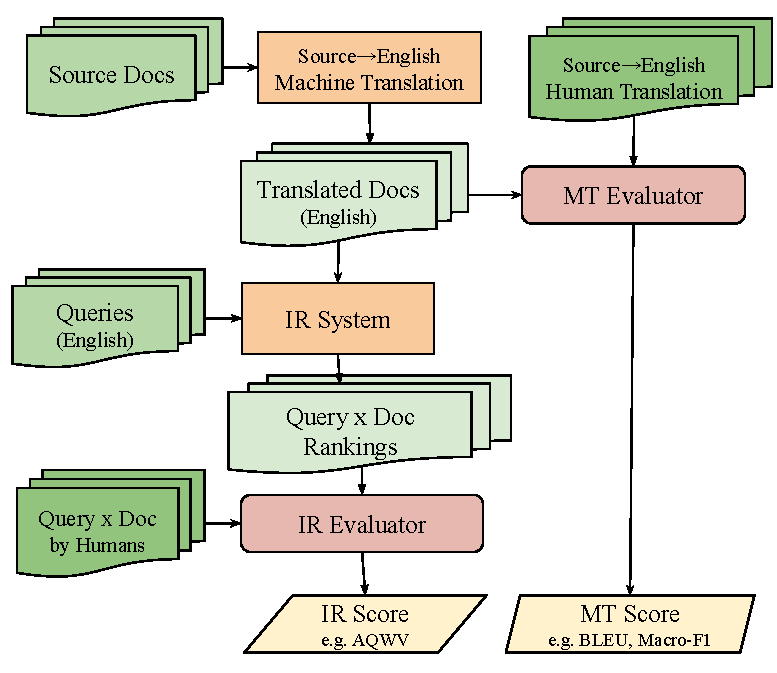
\includegraphics[width=0.9\linewidth,trim={0cm 0 0cm 0},clip]{img/CLIR-Pipe.pdf}
% to modify, goto https://docs.google.com/drawings/d/1ZrukLOtH3fQPyl9SkLWqrUqsbrSofDlSXC1tFwpYs2E/edit 
%\caption{Cross-lingual Information Retrieval system}
%\label{fig:clir-pipe}
%\end{figure}

An essential resource of this analysis is a dataset with human annotations for computing MT and IR performances.
%Specifically, this analysis requires datasets that have documents in source language and queries in target language,  along with the human translation of documents to calculate scores from MT measures, and human judgments of query to document relation to calculate IR performance.
%In addition, such datasets for a diverse set of languages are desired to verify the generalizabilty of findings.
%IARPA's Machine Translation for English Retrieval of Information in Any Language (MATERIAL) program\footnote{\myurl{https://www.iarpa.gov/index.php/research-programs/material/material-baa}} and made such datasets available, however only to its participants. 
We conduct experiments on two datasets: firstly, on data from the 2020 workshop on \textit{Cross-Language Search and Summarization of Text and Speech} (CLSSTS) \cite{clssts-2020}, and secondly, on data originally from Europarl, prepared by \citet{lignos-etal-2019-MT-IR} (Europarl).

%he restricted-access MATERIAL datasets using the systems submitted by MATERIAL performers where high-quality human judgments are available, and secondly, on publicly available datasets prepared by with a few assumptions on query-relevance judgments.

\subsubsection{CLSSTS Datasets}
\label{sec:material}

\begin{table*}[ht]
    \footnotesize
    \begin{tabular}{l l l r r r r r r }
 & Domain & IR Score & \bleu\ & \maf1 & \mif1 & \chrf1 & \blrtmn & \blrtmd \\\hline\hline

\multirow{4}{*}{LT-EN} 
& \multirow{2}{*}{In} 
  & AQWV & .429 & \insig.363 & \textbf{.508} & \insig.385 & .451  & .420 \\
& & MAP  & .495  & .429      & \textbf{.575} & .451       & .473  & .486 \\
& \multirow{2}{*}{In+Ext}
   & AQWV & \insig.345 & \textbf{.527} & .491  & .491 & .491 & .477 \\
&  & MAP  & \insig.273 & \insig\textbf{.455} & \insig.418 & \insig.418 & \insig.418 & \insig.404 \\\hline
\multirow{4}{*}{PS-EN}
  & \multirow{2}{*}{In} 
    & AQWV  & .559 & \textbf{.653} & .574 & .581 & .584 & .581  \\
  & & MAP   & .493 & \textbf{.632} & .487 & .494 & .558 & .554 \\
  & \multirow{2}{*}{In+Ext}
    & AQWV   & .589 & \textbf{.682} & .593 & .583 & .581 & .571 \\
  & & MAP    & .519 & \textbf{.637} & .523 & .482 & .536 & .526 \\\hline
\multirow{4}{*}{BG-EN}
 & \multirow{2}{*}{In} 
    & AQWV   & \insig.455 & \textbf{.550}   & .527  & \insig.382 & \insig.418  & .418 \\ 
 &  & MAP    &  .491      &  \textbf{.661}  & .564  &  .491       & .527       & .527 \\ 
 & \multirow{2}{*}{In+ext}
    & AQWV   & \insig.257 & \textbf{.500}       & \insig.330 & \insig.404 & \insig.367 & \insig.367 \\
 &  & MAP   & \insig.183 & \insig\textbf{.426} & \insig.257 & \insig.330 & \insig.294 & \insig.294 
\end{tabular} 
\caption{CLSSTS CLIR task: Kendall's $\tau$ between IR and MT metrics under study.
The rows with Domain=In are where MT and IR scores are computed on the same set of documents, whereas Domain=In+Ext are where IR scores are computed on a larger set of documents that is a superset of segments on which MT scores are computed.
\textbf{Bold} values are the best correlations achieved in a row-wise setting; values with \insig~ are \textit{not} significant at $\alpha=0.05$.}
\label{tab:material-kendall}
\end{table*}


CLSSTS datasets contain queries in English~(EN), and documents in many source languages along with their human translations, as well as query-document relevance judgments. 
We use three source languages: Lithuanian~(LT), Pashto~(PS), and Bulgarian~(BG).
The performance of this CLIR task is evaluated using two IR measures: Actual Query Weighted Value (AQWV) and Mean Average Precision (MAP).
AQWV\footnote{\href{https://www.nist.gov/system/files/documents/2017/10/26/aqwv\_derivation.pdf}{https://www.nist.gov/system/files/documents-/2017/10/26/aqwv\_derivation.pdf}} is derived from Actual Term Weighted Value (ATWV) metric \cite{wegmann2013ATWV}. 
%, being the official metric of MATERIAL program,
% by National Institute of Standards and Technology~(NIST). 
%The nature of AQWV is such that a higher score implies better CLIR performance. 
%Since the focus of this analysis is on MT evaluation methods and not the MT systems, we treat all MT systems as blackboxes for which internal details are unnecessary; however, we clarify that the MT systems used are representative of commonly used models such as convolutional \cite{gehring2017cnn} and Transformer~\cite{vaswani2017attention} NMT models, as well as once-popular syntax-based string-to-tree statistical MT~\cite{galley-etal-2004-sbmt}.


%The high level overview of our CLIR pipeline is shown in Figure \ref{fig:clir-pipe}:
%First, documents in source language are translated to English using a set of MT models. 
%Performance of all MT models is evaluated on the same set of documents using their corresponding human translations.
%The translated documents are indexed by an IR system, and the end-to-end performance on a set of queries is evaluated using AQWV metric with the help of human created judgments.
%Our CLIR system is based on \citet{boschee-etal-2019-saral}, which is competitive in the workshop on CLSSTS-2020~\cite{clssts-2020}.
%Since the CLIR system is also treated as a blackbox, the internals of CLIR is unnecessary and beyond the scope of this work.
We use a single CLIR system with the same IR settings for all MT models in the set,\footnote{Details of IR and MT models anonymized} and measure Kendall's $\tau$ between MT and IR measures.
The results, in Table~\ref{tab:material-kendall}, show that \maf1 is the strongest indicator of CLIR downstream task performance in five out of six settings.
AQWV and MAP have a similar trend in agreement to the MT metrics.
\chrf1 and BLEURT, which are strong contenders when generated text is directly evaluated by humans, do not indicate CLIR task performance as well as \maf1, as CLIR tasks require faithful meaning equivalence across the language boundary, and human translators can mistake fluent output for proper translations \cite{callison-burch-etal-2007-meta}. 
%Hence, we recommend the use of \maf1 when MT output is used in downstream tasks such as IR.



\subsubsection{Europarl Datasets} %\tg{pick more informative section name?}
\label{sec:lignos-etal}

\begin{table}[ht]
    \footnotesize
    \centering
\begin{tabular}{l@{\hspace{1mm}} r@{\hspace{1mm}} r@{\hspace{1mm}} r@{\hspace{1mm}} r@{\hspace{1.2mm}} r@{\hspace{1.2mm}} r}
 & \bleu\ & \maf1 & \mif1 & \chrf1 & $\overline{\text{BT}}$ & $\widetilde{\text{BT}}$ \\ \hline\hline
\multirow{1}{*}{ CS-EN } 
%& MAP  & \textbf{.950} & .933 & \textbf{.950} & \textbf{.950} & .900 & .933 \\
%& MAP  & \textbf{.95} & .93 & \textbf{.95} & \textbf{.95} & .90 & .93 \\
 & .850 & .867 & .850 & .850 & \textbf{.900} & .867 \\ 
%& RBO  & .85 & .87 & .85 & .85 & \textbf{.90} & .87 \\ \hline
\multirow{1}{*}{ DE-EN } 
%& MAP  & .862 & .895 & .862 & .874 & \textbf{.912} & .895 \\
%& MAP  & .86 & .90 & .86 & .87 & .91 & .90 \\
  & .900 & .900 & .900 & .912 & \textbf{.917} & .900 \\
%& RBO  & .90 & .90 & .90 & .91 & .92 & .90 \\
\end{tabular}  
\caption{Europarl CLIR task: Kendall's $\tau$ between MT metrics and RBO. $\overline{\text{BT}}$ and $\widetilde{\text{BT}}$ are short for \blrtmn\ and \blrtmd. All correlations are significant at $\alpha=0.05$.}
\label{tab:lignos-mtir-kendall} 
\end{table}


We perform a similar analysis to Section \ref{sec:material} but on another cross-lingual task set up by \citet{lignos-etal-2019-MT-IR} for Czech $\rightarrow$ English (CS-EN) and German $\rightarrow$ English (DE-EN), using publicly available data from the Europarl v7 corpus~\cite{koehn2005europarl}. 
%The IR model used is a term-based approach based on Okapi-BM25~\cite{jones2000probabilistic}.
%This task uses publicly available datasets; specifically documents from the Europarl v7 corpus~\cite{koehn2005europarl} for English, Czech, and German. 
This task differs from the CLSSTS task (Section \ref{sec:material}) in several ways.
Firstly, MT metrics are computed on test sets from the news domain, whereas IR metrics are from the Europarl domain. The domains are thus intentionally mismatched between MT and IR tests.
Secondly, since there are no queries specifically created for the Europarl domain, GOV2 TREC topics 701–850 are used as domain-relevant English queries.
And lastly, since there are no query-document relevance human judgments for the chosen query and document sets, the documents retrieved by BM25~\cite{jones2000probabilistic} on the English set for each query are treated as relevant documents for computing the performance of the CS-EN and DE-EN CLIR setup. 
As a result, IR metrics that rely on boolean query-document relevance judgments as ground truth are less informative, and we use Rank-Based Overlap (RBO; $p=0.98$) \cite{webber2010RBO} as our IR metric.

We perform our analysis on the same experiments as \citet{lignos-etal-2019-MT-IR}.\footnote{\myurl{https://github.com/ConstantineLignos/mt-clir-emnlp-2019}}
NMT models for CS-EN and DE-EN translation are trained using a convolutional NMT architecture \cite{gehring2017cnn} implemented in the FAIRSeq~\cite{ott2019fairseq} toolkit.
For each of CS-EN and DE-EN, a total of 16 NMT models that are based on different quantities of training data and BPE hyperparameter values are used.
%We report two IR metrics, namely: Rank-Based Overlap (RBO; $p=0.98$) \cite{webber2010RBO}, and Mean Average Precision (MAP), and their correlations with MT metrics.
The results in Table~\ref{tab:lignos-mtir-kendall} show that BLEURT has highest correlation in both cases.
Apart from the trained \blrtmd\ metric, \maf1 scores higher than the others on CS-EN, and is competitive on CS-EN. \maf1 is not the metric with highest IR task correlation in this setting, unlike in Section \ref{sec:material}, however it is competitive with \bleu\ and \chrf1, and thus a safe choice as a downstream task performance indicator. 



\section{Spotting Qualitative Differences between Supervised and Unsupervised NMT with \maf1}
\label{sec:unmt}

% \begin{tabular}{l rr | rr | rr| rr | rr | rr }
% \multicolumn{1}{}{} 
%      & \multicolumn{2}{c|}{\bleu}
%                   & \multicolumn{2}{c|}{\maf1} 
%                                  & \multicolumn{2}{c|}{\mif1} 
%                                               &\multicolumn{2}{c|}{\chrf1} 
%                                                             &\multicolumn{2}{c|}{\blrtmn} 
%                                                                                 &\multicolumn{2}{c}{\blrtmd} \\
%      & SN   & UN   & SN   & UN   & SN   & UN   & SN   & UN   & SN     & UN      & SN     & UN \\ \hline\hline
% DEEN & 32.7 & 33.9 & 38.5 & 33.6 & 58.7 & 57.9 & 59.9 & 58.0 & 0.211 & -0.026 & 0.285 & 0.067 \\
% ENDE & 24.0 & 24.0 & 24.0 & 23.5 & 47.7 & 48.1 & 53.3 & 52.0 &-0.134 & -0.204 &-0.112 & -0.197 \\
% FREN & 31.1 & 31.2 & 41.6 & 33.6 & 60.5 & 58.3 & 59.1 & 57.3 & 0.182 &  0.066 & 0.243 & 0.154 \\
% ENFR & 25.6 & 27.1 & 31.9 & 27.4 & 53.0 & 52.3 & 56.0 & 57.7 & 0.104 &  0.042 & 0.096 & 0.063 \\
% ROEN & 30.8 & 29.6 & 40.3 & 33.0 & 59.8 & 56.5 & 58.0 & 54.7 & 0.004 & -0.058 & 0.045 &-0.004 \\
% ENRO & 31.2 & 31.0 & 34.6 & 31.0 & 55.4 & 53.4 & 59.3 & 56.7 & 0.030 & -0.046 & 0.027 &-0.038 \\ 
% \end{tabular}%
\begin{table*}[ht!]
\centering
%\fontsize{8.5}{8.8}
%\selectfont
\footnotesize

\begin{tabular}{l @{\hspace{3mm}} r @{\hspace{1.5mm}} r @{\hspace{1.5mm}}r |  r@{\hspace{1.5mm}}r@{\hspace{1.5mm}}r |
  r@{\hspace{1.5mm}}r@{\hspace{1.5mm}}r | r@{\hspace{1.5mm}} r@{\hspace{1.5mm}} r | r@{\hspace{1.5mm}} r@{\hspace{1.5mm}} r | r @{\hspace{1.5mm}} r@{\hspace{1.5mm}} r}
& \multicolumn{3}{c|}{\bleu} & \multicolumn{3}{c|}{ \maf1 } & \multicolumn{3}{c|}{ \mif1 } & \multicolumn{3}{c|}{ \chrf1 } & \multicolumn{3}{c|}{ \blrtmn } & \multicolumn{3}{c}{ \blrtmd } \\ 
& SN & UN & $\Delta$ & SN & UN & $\Delta$ & SN & UN & $\Delta$ & SN & UN & $\Delta$ & SN & UN & $\Delta$ & SN & UN & $\Delta$ \\ \hline \hline
DE-EN & 32.7 & 33.9 & -1.2 & 38.5 & 33.6 & 4.9 & 58.7 & 57.9 &  0.8 & 59.9 & 58.0 &  1.9 & .211 & -.026 & .24 & .285 & .067 & .22 \\
EN-DE & 24.0 & 24.0 &  0.0 & 24.0 & 23.5 & 0.5 & 47.7 & 48.1 & -0.4 & 53.3 & 52.0 &  1.3 &-.134 & -.204 & .07 &-.112 &-.197 & .09 \\
FR-EN & 31.1 & 31.2 & -0.1 & 41.6 & 33.6 & 8.0 & 60.5 & 58.3 &  2.2 & 59.1 & 57.3 &  1.8 & .182 &  .066 & .17 & .243 & .154 & .09 \\
EN-FR & 25.6 & 27.1 & -1.5 & 31.9 & 27.3 & 4.6 & 53.0 & 52.3 &  0.7 & 56.0 & 57.7 & -1.7 & .104 &  .042 & .06 & .096 & .063 & .03 \\
RO-EN & 30.8 & 29.6 &  1.2 & 40.3 & 33.0 & 7.3 & 59.8 & 56.5 &  3.3 & 58.0 & 54.7 &  3.3 & .004 & -.058 & .06 & .045 & -.004 & .04 \\
EN-RO & 31.2 & 31.0 &  0.2 & 34.6 & 31.0 & 3.6 & 55.4 & 53.4 &  2.0 & 59.3 & 56.7 &  2.6 & .030 & -.046 & .08 & .027 & -.038 & .07 \\
\end{tabular} 

\caption{For each language direction, UNMT (UN) models have similar \bleu\ to SNMT (SN) models, and \chrf1 and \mif1 have small differences. 
However, \maf1 scores differ significantly, consistently in favor of SNMT. 
Both corpus-level interpretations of BLEURT support the trend reflected by \maf1, but the value differences are difficult to interpret.
}
\label{tab:unmt_vs_snmt}
\end{table*}

% \begin{figure*}[ht!]
%     \centering
%     \begin{subfigure}[b]{0.48\linewidth}
%     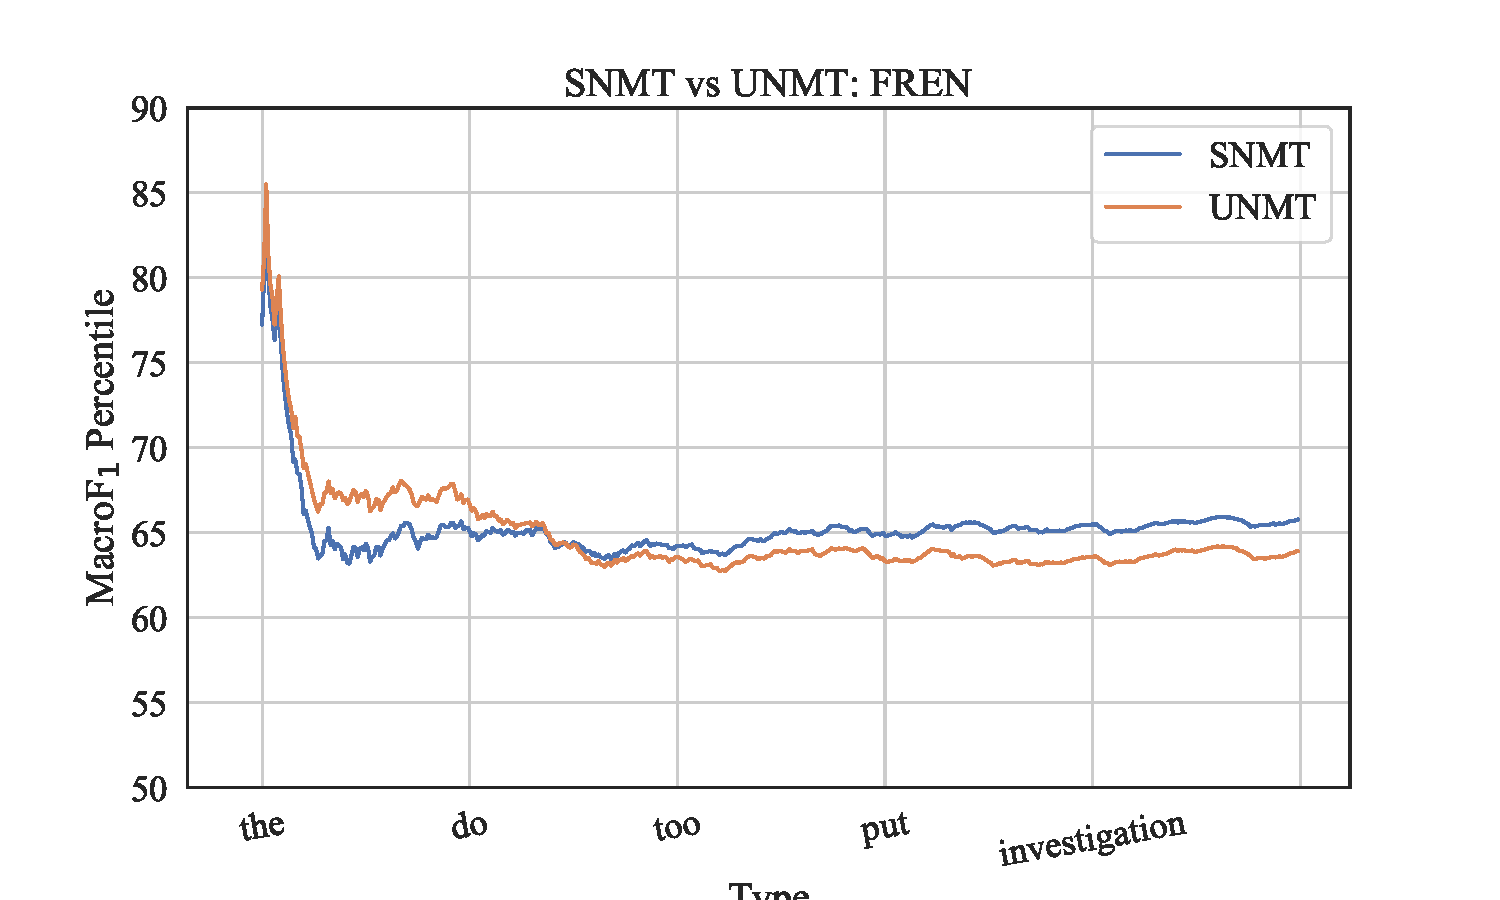
\includegraphics[width=\linewidth,trim={13mm 5mm 25mm 10mm},clip]{img/s_unmt-fren-maf1.pdf}
%     \label{fig:s-vs-u-fren}
%     \end{subfigure}
%     \hfill 
%     \begin{subfigure}[b]{0.48\linewidth}
%     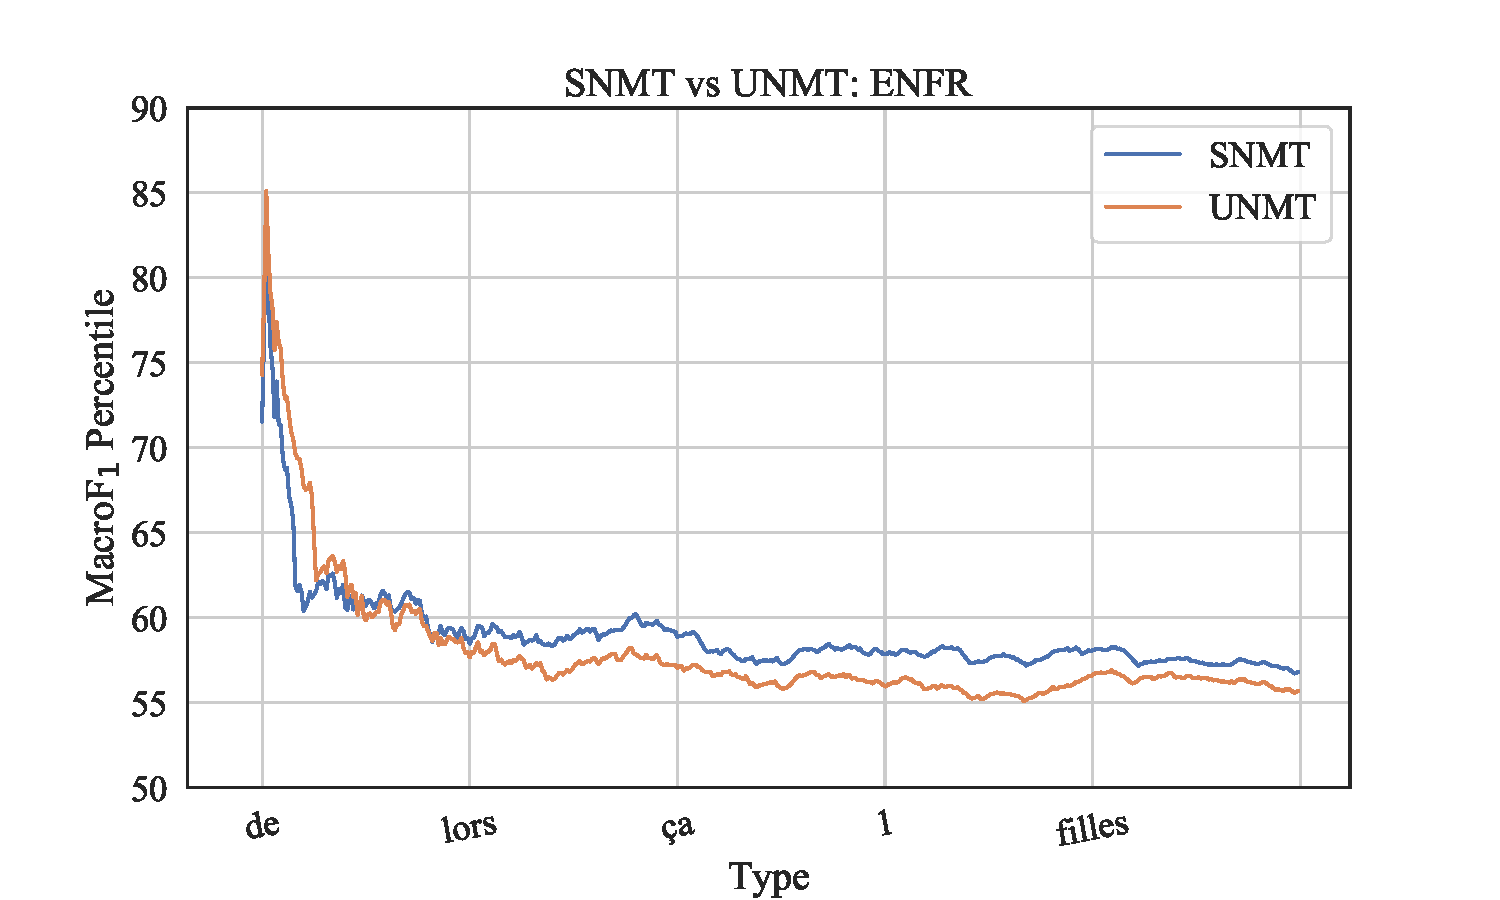
\includegraphics[width=\linewidth,trim={13mm 7mm 25mm 10mm},clip]{img/s_unmt-enfr-maf1.pdf}
%     \label{fig:s-vs-u-roen} 
%     \end{subfigure}

% \caption{\small Visualization of \maf1 between SNMT and UNMT. 
% Only the FREN and ENFR test sets for the most frequent 500 types are shown here, but the trend is similar on the other settings (see Figure~\ref{fig:snmt_vs_unmt-rest} in appendix).
% UNMT generally outperforms SNMT on the frequent types that contribute to fluency and hence score comparable \bleu\ scores, however, SNMT is generally better than UNMT on rare types hence SNMT scores higher \maf1. \tg{Explain that lines are viz of cumulative .}
% }
% \label{fig:snmt_vs_unmt}
% \end{figure*}

Unsupervised neural machine translation (UNMT) systems trained on massive monolingual data without parallel corpora have made significant progress recently \cite{Artetxe-2018-unmt-iclr,Lample-2018-unmt-iclr,lample-etal-2018-phrase-unmt,yang-etal-2018-unmt,conneau-NIPS2019-xlm,Song-2019-MASS,liu2020mbart}. 
In some cases, UNMT yields a \bleu\ score that is comparable with strong\footnote{though not, generally, the strongest} supervised neural machine translation (SNMT) systems. In this section we leverage \maf1 to investigate differences in the translations from UNMT and SNMT systems that have similar \bleu.

%\subsection{Experiment Settings}
We compare UNMT and SNMT for English $\leftrightarrow$ German (EN-DE, DE-EN), English $\leftrightarrow$ French (EN-FR, FR-EN), and English $\leftrightarrow$ Romanian (EN-RO, RO-EN).
All our UNMT models are based on XLM \citep{conneau-NIPS2019-xlm}, pretrained by \citet{XLM-UNMT-Models20}. 
We choose SNMT models with similar \bleu\ on common test sets by either selecting from systems submitted to previous WMT News Translation shared tasks~\cite{bojar-EtAl:2014:W14-33,bojar-EtAl:2016:WMT1} or by building such systems.\footnote{We were unable to find EN-DE and DE-EN systems with comparable \bleu\ in WMT submissions so we built standard Transformer-base~\cite{vaswani2017attention} models for these using appropriate training data to reach the desired \bleu\ performance. We report EN-RO results with diacritic removed to match the output of UNMT.} Specific SNMT models chosen are in the Appendix (Table~\ref{tab:unmt_vs_snmt2}).

 Table~\ref{tab:unmt_vs_snmt} shows performance for these language pairs using a variety of metrics. Despite comparable \bleu\ and only minor differences in \mif1 and \chrf1, SNMT models have consistently higher \maf1 and BLEURT than the UNMT models for all six translation directions. 
 
% We thus investigate \textit{why} there is such a divergence of relative opinion as measured by these autoeval methods.
% Note that \bleu\ and \chrf1 do not facilitate an type-wise comparison of MT models.
% Even though \blrtmn\ and \blrtmd\ show discrepancy between SNMT and UNMT, we are unable to interpret the difference and reason about it, which is concerning.
% However, \maf1 also provides performance per type, which are readily interpretable, on which macro-average is computed.

% Figure~\ref{fig:snmt_vs_unmt}, which is a visualization of \maf1 on most frequent 500 types, shows that UNMT outperforms SNMT on the frequent types such as stopwords which are weighed relatively highly in \bleu\ and other micro-averaged methods; however, SNMT is generally better than UNMT on the rest; hence, SNMT scores higher \maf1 than UNMT.
% Figure~\ref{fig:snmt_vs_unmt} is a simple explanation for the discrepancy between \maf1 and other micro-averaged methods in Table~\ref{tab:unmt_vs_snmt}.
% The take away from this section is that the easier interpretability aspect of \maf1 helps in uncovering the differences and flaws of MT models.
% For instance, it enabled us to find that the current UNMT systems produce fluent translations where as SNMT systems produce more adequate translations.

\input{45-su_nmt-qualitative}



%

\section{Biases in Model-based Evaluation}
\label{sec:model-bias}

Model-based metrics such as BLEURT sometimes outperform our simple statistical metrics. 
%The human judgments availability for a few high resource languages facilitate in the creation and utilization of model-based metrics in those settings. 
%However, on low resources settings, as our simple statistical methods do not need training, and hence readily usable. 
While these metrics are an interesting research direction, we are concerned by the following two key issues:
\begin{enumerate}[noitemsep,topsep=0pt]
    \item \textbf{Biases}: model-based metrics are based on learned word embeddings ~\cite{kaiwei-NIPS2016-emb-bias} and language modeling~\cite{sheng-etal-2019-nlg-bias} which are known to possess undesired biases \cite{mehrabi2019survey-bias}. 
    A bias of our concern is the marginalization of rare and minority concepts that affect the generation of rare types \cite{gowda2020finding}.
    \item \textbf{Non-interpretability}: the rationale behind any individual score from a model-based metric is opaque, while model-free metrics ultimately amount to an interpretable fraction of matched and unmatched tokens. 
\end{enumerate}

%if we are asked with ``why an output scored a certain score", the explanation one can provide is -- ``the evaluator model assigned that score and we do not know why". 
Table \ref{tab:bleurt-bias} contains two case studies that expose BLEURT's internal biases on certain word types.
Since many MT models are themselves non-interpretable and known to possess biases~\cite{prates2019-mt-bias}, using non-interpretable and biased evaluators in concurrence makes it even harder to discover and address the flaws in MT modeling.
In comparison, \maf1 is easily interpretable and offers the explanation of score as a composition of individual type performances.
%All these attributes are helpful to understand and address the flaws of MT models in practice. 
In addition, \maf1 treats all types equally, and hence it is free from the problems indicated in Table~\ref{tab:bleurt-bias}.

\begin{table}[ht]
    \centering
    \footnotesize
    \begin{tabular}{l l l }
Reference:& \multicolumn{2}{l}{You must be a doctor.} \\
Hypothesis: & \multicolumn{2}{l}{$\rule{1cm}{0.15mm}$ must be a doctor.} \\
    % & You &	~0.990 \\
    & He	&-0.735 \\
    %& Alexandra & -0.888 \\
    %& Alexander & -0.975 \\
    & Joe & -0.975 \\
    & Sue & -1.043 \\
    & She	 &-1.100 \\\hline
Reference:& \multicolumn{2}{l}{It is the greatest country in the world.} \\
Hypothesis:& \multicolumn{2}{l}{$\rule{1cm}{0.15mm}$ is the greatest country in the world.} \\
    % & It	& ~0.957 \\
    & France &	-0.022 \\
    & America	& -0.060 \\
    & Russia &	-0.161 \\
    %& China  & -0.166 \\
    %& USA    & -0.168 \\
    %& India   &	-0.211 \\
    & Canada  & -0.309 
    \end{tabular}
    \caption{BLEURT's internal biases on types lead to significant change in scores and hence rankings of hypothesis.
    BLEURT's score indicating that `He' is relatively better translation than `She' in the first example, and `France' is relatively better than `Canada' in the second example is not entirely objective.
    %On the other hand, sentence-level \bleu\ and \maf1 assigns same scores as expected by humans.
    %Even though these metrics perform well on some benchmark tasks,
    Using such metrics to select MT/ML models for real-world deployment is questionable.}
    \label{tab:bleurt-bias}
\end{table}

%\input{45-other-uses-tg}
%
\begin{table}[t]
% \resizebox{\textwidth}{!}{%
\centering
\footnotesize
\begin{tabular}{l rr|rr}
\multicolumn{1}{}{} & \multicolumn{2}{c|}{BLEU}   & \multicolumn{2}{c}{\maf1}\\
     & SNMT    & UNMT   & SNMT &  UNMT \\ \hline\hline
DEEN & 32.7    & 33.9   & 38.5  & 33.6 \\
ENDE & 24.0    & 24.0   & 24.0  & 23.5 \\
FREN & 31.1    & 31.2   & 41.6  & 33.6 \\
ENFR & 25.6    & 27.1   & 31.9  & 27.4 \\
ROEN & 30.8    & 29.6   & 40.3  & 33.0 \\
ENRO & 31.2    & 31.0   & 34.6  & 31.0 \\ 
\end{tabular}%
% }
\caption{Even though UNMT models score similar \bleu\ as SNMT models, they score significantly lower \maf1.}
\label{tab:unmt_vs_snmt}
\end{table}


\section{Application in Qualitative Evaluation of Unsupervised Neural Machine Translation}
\label{sec:unmt}
Unsupervised neural machine translation (UNMT) systems trained on massive monolingual data without parallel corpora have made significant progress recently \cite{Artetxe-2018-unmt-iclr,Lample-2018-unmt-iclr,lample-etal-2018-phrase-unmt,yang-etal-2018-unmt,conneau-NIPS2019-xlm,Song-2019-MASS,liu2020mbart}, in some cases yielding test BLEU that is comparable with supervised neural machine translation (SNMT) systems trained on millions of words of parallel data. In this section we leverage MacroF1 to investigate qualitative differences between UNMT and SNMT systems with similar BLEU.


\subsection{Experiment Settings}

We compare UNMT and SNMT for English $\leftrightarrow$ German (ENDE, DEEN), English $\leftrightarrow$ French (ENFR, FREN), and English $\leftrightarrow$ Romanian (ENRO, ROEN).
All our UNMT models are based on XLM \citep{conneau-NIPS2019-xlm}, pretrained by \citet{XLM-UNMT-Models20}. 
Our SNMT models are selected from the systems submitted to WMT shared tasks~\cite{bojar-EtAl:2014:W14-33,bojar-EtAl:2016:WMT1} which score similar \bleu\ to the available UNMT models.
For ENDE and DEEN, the WMT submissions' \bleu\ scores differ significantly from the available UNMT models.
Hence, we train a set of SNMT models for ENDE and DEEN using the standard Transformer-base~\cite{vaswani2017attention} architecture by varying training data and vocabulary sizes, and select the ones that scored similar \bleu\ with the available UNMT models. % following ablation in \citet{gowda2020finding}. 
%We compare these to SNMT models that have similar BLEU scores with their UNMT counterparts on common test sets.
%The other models are selected from submitted systems to WMT shared tasks in \cite{bojar-EtAl:2014:W14-33,bojar-EtAl:2016:WMT1}.\footnote{We do not use submitted systems for English $\leftrightarrow$ German because the submitted SNMT systems for NewsTest2019 have BLEU scores that differ significantly from our UNMT models. We thus carefully tune the data size and trained our own models that match UNMT on BLEU scores.} The SNMT models whose scores match with UNMT models are usually trained with smaller parallel corpora. 
Detailed description of chosen NMT models is in the appendix.\tg{section num?}
The \bleu\ scores of SNMT and UNMT systems are shown in Table~\ref{tab:unmt_vs_snmt}.

\subsection{Qualitative Differences between UNMT and SNMT}

\begin{table*}[t]
    \centering
    % \scalebox{0.8}{%
    \footnotesize
    \begin{tabular}{lllcc}
    
 & SNMT & UNMT & $\beneficial{S}{U}{\maf1}$&$\beneficial{S}{U}{BLEU}$\\ 
$1^{st}$ &\_synonym&	\textbf{untranslation}, \textbf{wrong\_noun}& 7.11E-02& 2.25E-02\\
$2^{nd}$ &\_synonym&	\textbf{untranslation}& 6.37E-02& 1.12E-02\\
$3^{rd}$ &\_synonym&	\textbf{untranslation}, \textbf{wrong\_noun}& 5.15E-02& 2.06E-02\\
$4^{th}$ &\_synonym, \_word\_order&	\textbf{dependency}, \textbf{truncation}, \textbf{word\_order}& 4.44E-02& -8.68E-04\\
$5^{th}$ &\_synonym, \_inflection&	\textbf{untranslation}, \textbf{wrong\_noun}& 4.43E-02& 2.54E-02\\
$6^{th}$ &\_inflection, \_word\_order&	\textbf{number}& 4.34E-02& 7.60E-03\\
$7^{th}$ &\textbf{day\_of\_week}, \_word\_order&	\_synonym, \textbf{day\_of\_week}, \textbf{weird\_char}& 4.09E-02& 1.76E-02\\
$8^{th}$ &\_synonym&	\textbf{untranslation}, \textbf{wrong\_noun}& 3.66E-02& 2.52E-02\\
$9^{th}$ &\_punctuation, \_synonym&	\textbf{truncation}& 3.66E-02& -1.06E-02\\
$10^{th}$ &\_synophrase, \_word\_order&	\_word\_order, \textbf{untranslation}& 3.61E-02& 5.54E-03\\

    \end{tabular}
    % }
    \caption{Problems for top 10 $\beneficial{S}{U}{\maf1}$ sentences such that \maf1 favors SNMT over UNMT for De-En. The labels starting with an underscores are problems that hurt evaluation metrics but are not real translation problems. \tg{Not sure if we need the numbers; seems too much info}}
    \label{tab:snmt_better_mf1}
\end{table*}



\begin{table*}[t]
    \centering
    % \scalebox{0.8}{
    \footnotesize
    \begin{tabular}{lllcc}
    
& SNMT & UNMT &$\deleterious{S}{U}{\maf1}$&$\deleterious{S}{U}{BLEU}$\\ 
$1^{st}$ &\textbf{unrelated\_other\_lang}&&5.48E-02&5.30E-03\\
$2^{nd}$ &\textbf{untranslation}&&4.46E-02&1.07E-02\\
$3^{rd}$ &\textbf{omit\_verb}, \textbf{untranslation}&	\textbf{wrong\_adj}, \textbf{wrong\_verb}&4.13E-02&1.15E-02\\
$4^{th}$ &\textbf{wrong\_name}&	\textbf{word\_order}& 4.00E-02&1.82E-02\\
$5^{th}$ &\_synophrase, \textbf{punctuation}&	\textbf{punctuation}, \textbf{untranslation}& 3.95E-02&5.36E-03\\
$6^{th}$ &\textbf{truncation}, \textbf{wrong\_meaning}&	\textbf{untranslation}& 3.51E-02&2.82E-03\\
$7^{th}$ &\_synonym, \textbf{wrong\_name}&	\textbf{omit\_verb}, \textbf{wrong\_adj}& 3.41E-02&5.76E-03\\
$8^{th}$ &\textbf{unk}, \textbf{untranslation}&	&3.40E-02&1.38E-02\\
$9^{th}$ &\_punctuation, \textbf{preposition}&&3.26E-02&1.87E-02\\
$10^{th}$ &\textbf{truncation}, \textbf{extra}&	\textbf{extra}&3.11E-02&7.43E-03\\ 
    \end{tabular}
    % }
    \caption{Problems for top 10 $\deleterious{S}{U}{\maf1}$ sentences such that MacroF1 favors UNMT over SNMT for De-En. \tg{Not sure we need the numbers; seems too much info}}
    \label{tab:unmt_better_mf1}
\end{table*}

% \jon{i think this is a quantitative/BLEU argument...for large data scenarios, SNMT models built on all the available parallel data result in higher bleu on test sets than UNMT models built on all the available monolingual data (that can be leveraged). The question we're asking in this investigation is, at comparable BLEU, do SNMT and UNMT exhibit qualitative differences, and can these differences be detected by other metrics?}.

We observe in Table~\ref{tab:unmt_vs_snmt} that despite the comparable \bleu\ scores,  SNMT models have consistently higher \maf1 than the UNMT models for all six translation directions. 
We thus investigate \textit{why} the translation behaviors of SNMT and UNMT models on the same input sentences lead to a divergence of relative opinion as measured by these two metrics.

% \jon{Another quantitative argument for better...using MacroF1 (which presumably has been previously introduced...in your talk you'll have to discuss this, probably in a different order) indicates the performance is not in fact comparable. So the investigative question is, what contributes to this difference of opinion (i.e. what translation errors affect MacroF1 but don't affect BLEU), and what are the qualitative properties of these contributions?}  

% \jon{trying to explain the sentence removal delta scheme...}

Since \bleu\ and \maf1 are corpus-level metrics, we use a \textit{maximum difference discriminator} approach for illustrative sentence selection to manually investigate the differences at sentence level.
The approach is defined as follows: Consider a source-language corpus $X$ and a corpus of translations $C$ with corpus-level metric $M$ that produces score $C_M$. 
For some $x \in X$, $C[x]$ is the translation of $x$ in $C$.
Let $C^{-x} = C \setminus \{C[x]\}$ and $C^{-x}_M$ be the score according to $M$ of $C^{-x}$ (i.e. as if $x$ is not part of the input and its reference is not part of the reference set). 
Then let $\scoredel{C}{x}{M} = C^{-x}_M - C_M$; if $\scoredel{C}{x}{M} > 0$ we say (the translation of) $x$ is \textit{deleterious} to $C$ with respect to $M$, since the inclusion of $C[x]$ lowers the overall score.
Now, consider another corpus of translations of $X$, $K$. 
We define the \textit{deleteriousness of item $x$} that compares $C$ and $K$ with respect to $M$ as $\deleterious{C}{K}{M}(x)$:

\tg{Let $X$, $Y$, and $H$, be a corpus of source, reference, and hypothesis, respectively. Let $M$ be a corpus-level measure such that $M(H, Y) \in \mathbb{R}$ and a higher value implies better translation quality. 
Let $H[x]$ and $Y[x]$ are hypothesis and reference translations $\forall x \in X$.
Let $H_{-x} = H \setminus \{H[x]\}$, and similarly $Y_{-x}$. 
Then, $M(H_{-x}, Y_{-x})$ be the corpus-level score by excluding the hypothesis and reference sentences of $x$.
We define, $\scoredel{H}{x}{M} = M(H_{-x}, Y_{-x}) - M(H, Y)$.
If $\scoredel{H}{x}{M} > 0$, $x$ is \textit{deleterious} to $H$ with respect to $M$ as the inclusion of $H[x]$ into $H$ lowers the corpus-level score.
Now consider another set of translations, $K$, of the same $X$ from a different MT model. 
We define the \textit{deleteriousness of item $x$} that compares both $H$ and $K$  translation with respect to the method $M$ as $\deleterious{H}{K}{M}(x)$:
}
% We define the \textit{maximal net deleterious item} that compares $C$ and $K$ with respect to $M$ as $\deleterious{C}{K}{M}$: \jon{need to broaden this to something like general deleteriousness and then a way of determining nth most deleterious}

% \begin{equation}
% \deleterious{C}{K}{M} = \mbox{argmax}_{x \in X} \scoredel{C}{x}{M} - \scoredel{K}{x}{M}
% \label{eq:deleterious}
% \end{equation}

\begin{equation}
\deleterious{C}{K}{M}(x) = \scoredel{C}{x}{M} - \scoredel{K}{x}{M}
\label{eq:deleterious}
\end{equation}

\noindent such that a sentence that is very deleterious to $C$ \textit{and} very beneficial to $K$ would be selected by $\mbox{argmax}_{x \in X}\deleterious{C}{K}{M}(x)$.
Let $C$ and $K$ be corpora of translations generated via different approaches (e.g. SNMT vs. UNMT). 
We use $\mbox{argmax}_{x \in X}\deleterious{C}{K}{M}$ to find behaviors that are regarded as negative to $M$ being exhibited by $C$ but not by $K$.
An analogous measure, $\mbox{argmax}_{x \in X}\ \beneficial{C}{K}{M}(x)$ finds the most \textit{beneficial} item in $C$ but not in $K$, essentially flipping the signs in Equation~\ref{eq:deleterious}.

% \jon{I think then the evaluation you want to do is to find the change-makers according to macrof1 and see what they do to bleu. the opposite can also be studied}

When we manually examine the top 10 and bottom 10 scored outputs for German-English using $\beneficial{S}{U}{\maf1}$ and $\beneficial{S}{U}{\bleu}$, we find that when SNMT is better, UNMT has more untranslated words while SNMT only has non-important problems like switching word order in a reasonable way or using synonyms (Table~\ref{tab:snmt_better_mf1}). When UNMT is better in terms of metrics, on the other hand, it still has some untranslated words, while SNMT's problems are mixures of wrong words, synonym, and word order (Table~\ref{tab:unmt_better_mf1}).

\subsection{Qualitative Differences between \bleu\ and \maf1}


% In order to see how MacroF1 and BLEU differ qualitatively, we look at some extreme cases of translations where MacroF1 and BLEU's rank differ most. We first rank $\beneficial{S}{U}{MacroF1}$ and $\beneficial{S}{U}{BLEU}$ descending separately and aquire the rank differences with

% $$\Delta\mathit{Rank} = \mathit{Rank}(\beneficial{S}{U}{MacroF1}) - \mathit{Rank}(\beneficial{S}{U}{BLEU})$$

In order to see how two metrics $M_1$ and $M_2$ differ qualitatively, we look at some extreme cases of translations where $M_1$ and $M_2$'s rank differ most. We first rank $\beneficial{C}{K}{M_1}$ and $\beneficial{C}{K}{M_2}$ descending separately and define \textit{favorness of $x$ in corpus $C$ by $M_2$ instead of $M_1$} as the rank differences

\begin{equation}
\begin{split}
    \deleterious{M_1}{M_2}{Rank}(x) = &\mathit{Rank}(\beneficial{C}{K}{M_1}(x)) \\
&- \mathit{Rank}(\beneficial{S}{U}{M_2}(x))
\end{split}
\label{eq:favorness}
\end{equation}

The lowest $\deleterious{M_1}{M_2}{Rank}(x)$ (ranked to the front) are sentences whose translations in $C$ are favored by $M_1$ while translations in $K$ are favored by $M_2$, and the highest $\deleterious{M_1}{M_2}{Rank}(x)$ (ranked to the back) are opposite and are sentences whose translations in $C$ are favored by $M_2$ while translations in $K$ are favored by $M_1$.

We manually examine sentences with the top 10 $\deleterious{\maf1}{\bleu}{Rank}(x)$ and $\beneficial{\maf1}{\bleu}{Rank}(x)$ scores (sentences for whom \maf1 and \bleu\ disagree the most), and conclude the following trend in how \maf1 favors SNMT that is more adequate than UNMT (examples shown in Table~\ref{tab:diff_mf1_bleu}):

\begin{table*}[htbp]
    \centering
    \resizebox{\textwidth}{!}{%
    \begin{tabular}{l|l}
    
$3^{rd}$& $\beneficial{S}{U}{MacroF1}$ : 0.014, $\deleterious{S}{U}{BLEU}$: 0.025 \\\hline
Src & Zu den Finanzierungsmöglichkeiten für Langzeitpflege gehören eine traditionelle \colorbox{pink}{Pflegeversicherung}, eine hybride \\
&kapitalbindende Lebensversicherung zur Abdeckung dieser Ausgaben oder eine Selbstversicherung mit dem eigenen \\
&Vermögen – solange Sie das Geld dafür haben.\\\hline
Ref & Your funding choices for long-term care can include a traditional long-term care insurance policy, a hybrid cash-value \\
&life insurance policy to help cover these expenses or self-insuring with your own wealth - as long as you have the money.\\\hline
SNMT& Financing opportunities for long-term care include traditional care insurance, hybrid capital-binding life insurance to \\
&cover this spending, or self-insurance with your own assets – as long as you have the money for it.,,,,,,,,,,,,,,,,, etc.\\\hline
UNMT& Among the financing options for long-term care are a traditional \colorbox{pink}{Pflegeversicherung}, a hyper-fat equity binoculars to \\
&cover these expenses or a self-fund with your own wealth - as long as you have the money for it.\\\hline
Problems&SNMT: \_synonym, \_punctuation, omit\_adj. UNMT: \_synonym, \textbf{untranslation}, wrong\_adj, wrong\_noun.\\\hline\hline

$4^{th}$& $\beneficial{S}{U}{\maf1}$: 0.037, $\deleterious{S}{U}{\bleu}$: 0.011 \\\hline
Src & Trotzdem war der Ton von Ri's Rede dramatisch anders als letztes Jahr, als er es der U.N. berichtete. Die Generalversa-\\
&mmlung, die das US-Festland mit Nordkoreas Raketen ins Visier nahm, war unvermeidlich, nachdem ``Mr. Evil President" \\
&Trump Kim als ``Raketenmann" auf einer Selbstmordmission bezeichnete.\\\hline

Ref & Even so, the tone of Ri's speech was dramatically different from last year, when he told the U.N. General Assembly \colorbox{yellow}{that} \\
&\colorbox{yellow}{targeting the U.S. mainland with North Korea's rockets was inevitable after ``Mr Evil President" Trump called Kim a} \\
&\colorbox{yellow}{``rocket man" on a suicide mission.}\\\hline

SNMT& However, the tone of Ri's speech was dramatically different from last year when he reported it to the U.N., and the \\
&General Assembly, targeting the US mainland with North Korea ' s missiles, was inevitable after ``Mr. Evil President " \\
&Trump called Kim a`` missile man " on a suicide mission.\\\hline

UNMT& Nonetheless, the tone of Ri's speech was dramatically different from last year when he reported it to the U.N. General \\
&Assembly.\\\hline

Problems&SNMT: \_punctuation, \_synonym. UNMT: \textbf{truncation}.\\


    \end{tabular}
    }
    \caption{Cases to show different qualities MacroF1 and BLEU value. When the ``diff" is positive, it means the metrics thinks SNMT is better. When the ``diff" is negative, it means the metrics thinks UNMT is better. a) The 3rd ranked sentence has untranslation in UNMT translation that is detected by MacroF1. b) The 4th ranked sentence has the whole second half of the sentence after ``General Assembly" that is truncated in UNMT's translation, and MacroF1 prefers SNMT's translation while BLEU still prefers UNMT. }
    \label{tab:diff_mf1_bleu}
\end{table*}

% \textbf{Pros of MacroF1:}

\begin{itemize}
    \item \maf1 tends to find out untranslations because they have equal weights for each word. Untranslations are rare words and get weighted more. (e.g. 3rd ranked sentence where \maf1 favors SNMT but \bleu favors UNMT.) % \#1564 (3rd)
    \item \maf1 favors the sentence without truncation which also appears more in UNMT. (e.g. 4th ranked sentence where \maf1 favors SNMT but BLEU favors UNMT.)  %\#758 (4th) \#921 (1996th)
\end{itemize}



\section{Related Work}

\subsection{MT Metrics}
 Many metrics have been proposed for MT evaluation, which we broadly categorize into \textit{model-free} or \textit{model-based}. Model-free metrics compute scores based on translations but have no significant parameters or hyperparameters that must be tuned \textit{a priori}; these include  \bleu\ \cite{papineni-etal-2002-bleu}, NIST \cite{doddington2002-nist}, TER \cite{snover2006TER}, and \chrf1 \cite{popovic-2015-chrf}.  Model-based metrics have a significant number of parameters and, sometimes, external resources that must be set prior to use. These include METEOR \cite{banerjee-lavie-2005-meteor},  BLEURT \cite{sellam-etal-2020-bleurt}, YiSi \cite{lo-2019-yisi}, ESIM \cite{mathur-etal-2019-ESIM}, and BEER \cite{stanojevic-simaan-2014-beer}. Model-based metrics require significant effort and resources when adapting to a new language or domain, while model-free metrics require only a test set with references. 

\citet{mathur-etal-2020-tangled} have recently evaluated the utility of popular metrics and recommend the use of either \chrf1 or a model-based metric instead of \bleu. 
We compare our \maf1 and \mif1 metrics with \bleu, \chrf1, and BLEURT \cite{sellam-etal-2020-bleurt}.
%Note from Figure~\ref{fig:bleu-damage} that \bleu\ and \chrf1 are implicitly micro-averaged measures similar to \mif1.

%While the \textit{model-based} methods are an interesting research direction, we are concerned about the following two key issues.
%Firstly, regarding the \textit{undesired biases}: model-based methods are based on learned representations~\cite{kaiwei-NIPS2016-emb-bias} and language modeling~\cite{sheng-etal-2019-nlg-bias} which are known to possess undesired data-based biases~\cite{mehrabi2019survey-bias}.
%A bias of our primary concern is a marginalization of rare and minority concepts that affect the generation of rare words from Long Tail \cite{gowda2020finding}.
%Secondly, regarding \textit{uninterpretability}: model-based methods offer only the scores without any reliably established way to reason about those scores. 
%if we are asked with ``why an output scored a certain score", the explanation one can provide is -- ``the evaluator model assigned that score and we do not know why". 
%Since many MT models are themselves uninterpretable and known to possess biases~\cite{prates2019-mt-bias}, using uninterpretable and possibly biased evaluators in concurrence makes the discovery and addressing of flaws in MT models even harder.
%Such a faith on uninterpretable entities in evaluation is against the spirit of science.
%The methods we have proposed in this work are simple, interpretable, based on well established classifier evaluation methods, and offer performance breakdown to the level of individual types that assist in a detailed analysis. 

%An example analysis between supervised and unsupervised NMT is given in Section~\ref{sec:unmt}.
    

\subsection{Rare Words are Important}
\label{sec:rare-words}
That natural language word types roughly follow a Zipfian distribution is a well known phenomenon \cite{zipf1949human,powers-1998-zipf-apps}.
The frequent types are mainly so-called ``stop words,'' function words, and other low-information types, while most content words are infrequent types.
%whereas the right side contains rare content words.
%Even though frequent types occur several orders of magnitude more frequently than others, they carry relatively less information~\cite{shannon1948mathematical}.
To counter this natural frequency-based imbalance, statistics such as inverted document frequency (IDF) are commonly used to weigh the \textit{input} words in applications such as information retrieval~\cite{Jones72specificity}.
%IDF, being inversely proportional to frequencies, emphasizes the infrequent types, as they are more `useful' than the frequent types.
In NLG tasks such as MT, where words are the \textit{output} of a classifier, there has been scant effort to address the imbalance.
\citet{doddington2002-nist} is the only work we know of in which the `information' of an n-gram is used as its weight, such that rare n-grams attain relatively more importance than in BLEU. 
We abandon this direction for two reasons:
Firstly, as noted in that work, \textit{large amounts of data are required to estimate n-gram statistics}.
Secondly, unequal weighing is a bias that is best suited to datasets where the weights are derived from, and such biases often do not generalize to other datasets.
Therefore, unlike \citet{doddington2002-nist}, we assign equal weights to all n-gram classes, and in this work we limit our scope to unigrams only.

While \bleu{} is a precision oriented measure, METEOR \cite{banerjee-lavie-2005-meteor} and CHRF \cite{popovic-2015-chrf} include both precision and recall similar to our methods.
However, neither of these measures try to address the natural imbalance of class distribution. 
BEER \cite{stanojevic-simaan-2014-beer} and METEOR \cite{denkowski-lavie-2011-meteor1.3} make an explicit distinction between function and content words; such a distinction inherently captures the frequency differences since the function words are often frequent and content words are often infrequent types. However, doing so requires the construction of potentially expensive linguistic resources. This work does not make any explicit  distinction and uses naturally occurring type counts to effect a similar result.

\subsection{F-measure as an Evaluation Metric}
F-measure \cite{Rijsbergen-1979-F-meas, chinchor-1992-F-meas} is extensively used as an evaluation metric in classification tasks such as part-of-speech tagging, information extraction, named entity recognition, and sentiment analysis \cite{derczynski-2016-f-score}.
Viewing MT as a multi-class classifier is a relatively new paradigm \cite{gowda2020finding}, and evaluating MT solely as a multi-class classifier as proposed in this work is not an established practice.
However, we find that the $F_1$ measure is sometimes used for various analyses when \bleu{} and others are inadequate: The compare-mt tool \citep{neubig-etal-2019-compareMT} supports comparison of MT models based on $F_1$ measure of individual types.
\citet{gowda2020finding} use $F_1$ of individual types to uncover frequency-based bias in MT models.
\citet{sennrich-etal-2016-bpe} use corpus-level \textit{unigram $F_1$} in addition to \bleu\ and \chrf{}, however, corpus-level $F_1$ is computed as \mif1. %In this work, \maf1 is our primary focus, and we use \mif1 for  only.
To the best of our knowledge, there is no previous work that clearly formulates the differences between micro- and macro- averages, and justifies the use of \maf1 for MT evaluation. 


\section{Discussion and Conclusion}
We have evaluated NLG in general and MT specifically as a multi-class classifier, and illustrated the differences between micro- and macro- averages using \mif1 and \maf1 as examples (Section~\ref{sec:mt-as-cls}).
\maf1 captures semantic adequacy better than \mif1 (Section~\ref{sec:webnlg}).
\bleu, being a micro-averaged measure, served well in an era when generating fluent text was at least as difficult as generating adequate text. Since we are now in an era in which fluency is taken for granted and semantic adequacy is a key discriminating factor, macro-averaged measures such as \maf1 are better at judging the generation quality of MT models (Section~\ref{sec:wmt-metrics}).
We have found that another popular metric, \chrf1, also performs well on direct assessment,
%as it uses character level n-grams that offer robustness to morphological variations
however, being an implicitly micro-averaged measure, it does not perform as well as \maf1 on downstream CLIR tasks (Section~\ref{sec:material}).
Unlike BLEURT, which is also adequacy-oriented, \maf1 is directly interpretable, does not require retuning on expensive human evaluations when changing language or domain, and does not appear to have uncontrollable biases resulting from data effect.
%We have also included a comparison to BLEURT, but we reserve our concerns regarding the non-transparency and biased evaluation by such model-based methods. %(Section~\ref{sec:model-bias}). 
%\maf1 is competitive to alternative methods and has the advantage of 
It is both easy to understand and to calculate, and is  
inspectable, enabling fine-grained analysis at the level of individual word types. These attributes make it a useful metric for understanding and addressing the flaws of current models. For instance, we have used \maf1 to compare supervised and unsupervised NMT models at the same operating point measured in \bleu, and determined that supervised models have better adequacy than the current unsupervised models (Section~\ref{sec:unmt}).

Macro-average is a useful technique for addressing the importance of the long tail of language, and \maf1 is our first step in that direction; we anticipate the development of more advanced macro-averaged metrics that take advantage of higher-order and character n-grams in the future. 

\section{Ethical Consideration}

Since many machine learning models including NMT are themselves opaque and known to possess data-induced biases~\cite{prates2019-mt-bias}, using opaque and biased evaluation metrics in concurrence makes it even harder to discover and address the flaws in modeling.
Hence, we have raised concerns about the opaque nature of the current model-based evaluation metrics, and demonstrated examples displaying unwelcome biases in evaluation. We advocate the use of the \maf1 metric, as it is easily interpretable and offers the explanation of score as a composition of individual type performances.
%All these attributes are helpful to understand and address the flaws of MT models in practice. 
In addition, \maf1 treats all types equally, and has no parameters that are directly or indirectly estimated from data sets. Unlike \maf1, \mif1 and other implicitly or explicitly micro-averaged metrics assign lower importance to rare concepts and their associated rare types. 
The use of micro-averaged metrics in real world evaluation could lead to marginalization of rare types.

% underrepresented ?
%Hence, we strongly recommend the use of transparent, macro-averaged metrics such as \maf1. 

\textit{Failure Modes:}
The proposed \maf1 metric is not the best measure of fluency of text. 
Hence we suggest caution while using \maf1 to draw fluency related decisions. \maf1 is inherently concerned with \textit{words}, and assumes the output language is easily segmentable into word tokens. Using \maf1 to evaluate translation into alphabetical languages such as Thai, Lao, and Khmer, that do not use white space to segment words, requires an effective tokenizer. Absent this the method may be ineffective; we have not tested it on languages beyond those listed in Section~\ref{sec:apphuman}.

\textit{Reproducibility:}
Our implementation of \maf1 and \mif1 has the same user experience as \bleu{} as implemented in \textsc{SacreBleu}; signatures are provided in Section~\ref{sec:appmetrics}. 
In addition, our implementation is  computationally efficient, and has the same (minimal) software and hardware requirements as \bleu{}. 
We plan to make our implementation available to the public after the anonymity period. All data for MT and NLG human correlation studies is publicly available and documented. Data for reproducing the IR experiments in Section~\ref{sec:lignos-etal} is also publicly available and documented. The data for reproducing the IR experiments in Section~\ref{sec:material} is only available to participants in the CLSSTS shared task. 
% by submitting a pull request to the upstream \textsc{SacreBleu} repository

\textit{Climate Impact:} Our proposed metrics are on par with \bleu{} and such model-free methods, which consume significantly less energy than most model-based evaluation metrics.

%the problems indicated in Table~\ref{tab:bleurt-bias}.
%\section*{Acknowledgements}

Thanks to Joel Barry, Shantanu Agarwal, and Scott Miller helping with MATERIAL CLIR experiments.
Thanks to Daniel Cohen for discussions on IR evaluation methods. 


\bibliography{80-refs}
\bibliographystyle{acl_natbib}

\clearpage
\appendix

\section{Metrics Reproducibility}
\label{sec:appmetrics}

\bleu\ scores reported in this work are computed with the \textsc{SacreBleu} library and has signature \texttt{\small BLEU+case.mixed+lang.<xx>-<yy>+numrefs.1 +smooth.exp+tok.<TOK>+version.1.4.13}, where \texttt{<TOK>} is \texttt{zh} for Chinese, and \texttt{13a} for all other languages. \maf1 and \mif1 use the same tokenizer as \bleu.
\chrf1 is also obtained using \textsc{SacreBleu} and has signature \texttt{\small chrF1+lang.<xx>-<yy>+numchars.6 +space.false +version.1.4.13}.
BLUERT scores are from the \textit{base} model \citet{sellam-etal-2020-bleurt}, which is fine-tuned on WMT Metrics ratings data from 2015-2018.
The BLEURT model is retrieved from \myurl{https://storage.googleapis.com/bleurt-oss/bleurt-base-128.zip}.


\section{Agreement with WMT Human judgments}
\label{sec:apphuman}

Tables \ref{tab:wmt19-kendall}, \ref{tab:wmt18-kendall}, and \ref{tab:wmt17-kendall} provide $\tau$ between MT metrics and human judgments on WMT Metrics task 2017--2019. 
$\star$\bleu\ is based on pre-computed scores in WMT metrics package, whereas \bleu\ is based on our recalculation using \textsc{SacreBleu}. 
Values marked with \insig are not significant at $\alpha=0.05$, and hence corresponding rows are excluded from the calculation of mean, median, and standard deviation.

Since \maf1 is the only metric that does not achieve statistical significance in the WMT 2019 EN-ZH setting, we carefully inspected it.
Human scores for this setting are obtained without looking at the references by bilingual speakers \cite{WMT19-metrics-proceedings}, but the ZH references are found to have a large number of bracketed EN phrases, especially proper nouns that are rare types.
When the text inside these brackets is not generated by an MT system, \maf1 naturally penalizes heavily due to the poor recall.
Since other metrics assign lower importance to poor recall of such rare types, they achieve relatively better correlation to human scores than \maf1. 
However, since the $\tau$ values for EN-ZH are relatively lower than the other language pairs, we conclude that poor correlation of \maf1 in EN-ZH is due to poor quality references.
Some settings did not achieve statistical significance due to a smaller sample set as there were fewer MT systems submitted, e.g. 2017 CS-EN.

\begin{table}[ht]
    \footnotesize
    \centering
\begin{tabular}{l @{\hspace{1.5mm}} r @{\hspace{1.5mm}} r @{\hspace{1.5mm}} r @{\hspace{1.5mm}} r @{\hspace{1.5mm}} r}
 & $\star$\bleu & \bleu & \maf1 & \mif1 & \chrf1 \\ \hline \hline
DE-CS & .855 & .745 & .964 & .917 & \textbf{.982}  \\
DE-EN & .571 & .655 & .723 & .695 & \textbf{.742} \\
DE-FR & .782 & .881 & \textbf{.927} & .844 & .915 \\
EN-CS & .709 & \textbf{.954} & .927 & .927 & .908  \\
EN-DE & .540 & .752 & .741 & .773 & \textbf{.824} \\
EN-FI & .879 & .818 & .879 & .848 & \textbf{.923}  \\
EN-GU & .709 & .709 & .600 & \textbf{.734} & .709  \\
EN-KK & .491 & .527 & \textbf{.685} & .636 & .661  \\
EN-LT & .879 & .848 & \textbf{.970} & .939 & .881 \\
EN-RU & .870 & .848 & \textbf{.939} & .879 & .930  \\
FI-EN & .788 & .809 & \textbf{.909} & .901  & .875 \\
FR-DE & \textbf{.822} & .733 & .733 & .764  & .815 \\
GU-EN & .782 & .709 & .855 & .891 & \textbf{.945}  \\
KK-EN & \textbf{.891} & .844 & .796 & .844 & .881 \\
LT-EN & .818 & \textbf{.855} & .844 & \textbf{.855}  & .833 \\
RU-EN & .692 & .729 & .714 & \textbf{.780} & .757 \\
ZH-EN & .695 & .695 & \textbf{.752} & .676 & .715 \\ \hline
Median & .782 & .752 & .844 & .844 & .875\\
Mean & .751 & .771 & .821 & .818 & .841  \\
SD & .124 & .101 & .112 & .093 & .095  \\ \hline
EN-ZH & \textbf{.606} & \textbf{.606} & \insig.424 & .595 & .594 \\ \hline
Wins & 3 & 3 & 6 & 3 & 5 
\end{tabular} 
\caption{ WMT19 Metrics task: Kendall's $\tau$ between metrics and human judgments.}
\label{tab:wmt19-kendall}
\end{table}
%\vspace{2px}
\begin{table}[ht]
    \footnotesize
    \centering
\begin{tabular}{l @{\hspace{1.5mm}} r @{\hspace{1.5mm}} r @{\hspace{1.5mm}} r @{\hspace{1.5mm}} r @{\hspace{1.5mm}} r}
 & $\star$\bleu & \bleu & \maf1 & \mif1 & \chrf1 \\ \hline \hline
DE-EN & .828 & .845 & .917 & .883 & \textbf{.919}  \\
EN-DE & .778 & .750 & \textbf{.850} & .783 & .848  \\
EN-ET & .868 & .868 & .934 & .906 & \textbf{.949}  \\
EN-FI & .901 & .848 & .901 & .879 & \textbf{.945}  \\
EN-RU & .889 & .889 & \textbf{.944} & .889 & .930  \\
EN-ZH & .736 & .729 & .685 & \textbf{.833} & .827 \\
ET-EN & .884 & .900 & .884 & .878 & \textbf{.904}  \\
FI-EN & .944 & .944 & .889 & .915 & \textbf{.957}  \\
RU-EN & .786 & .786 & \textbf{.929} & .857 & .869 \\
ZH-EN & .824 & \textbf{.872} & .738 & .780 & .820  \\ 
EN-CS & \textbf{1.000} & \textbf{1.000} & .949 & \textbf{1.000} & .949  \\ \hline

Median & .868 & .868 & .901 & .879 & .919  \\
Mean   & .858 & .857 & .875 & .873 & .902  \\
SD     & .077 & .080 & .087 & .062 & .052  \\ \hline

TR-EN & \insig.200 & \insig.738 & \insig.400 & \insig.316 & \insig.632 \\
EN-TR & \insig.571 & \insig.400 & .837 & \insig.571 & \textbf{.849}  \\
CS-EN & \insig.800 & \insig.800 & \insig.600 & \insig.800 & \insig.738 \\ \hline
Wins &  1  &  2 & 3 &  2 & 6
\end{tabular}
\caption{ WMT18 Metrics task: Kendall's $\tau$ between metrics and human judgments.}
\label{tab:wmt18-kendall}

\end{table}
%\vspace{2px}
\begin{table}[ht]
    \footnotesize
    \centering
\begin{tabular}{l @{\hspace{1.5mm}} r @{\hspace{1.5mm}} r @{\hspace{1.5mm}} r @{\hspace{1.5mm}} r @{\hspace{1.5mm}} r}
 & $\star$\bleu & \bleu & \maf1 & \mif1 & \chrf1 \\ \hline \hline
DE-EN & .564 & .564 & .734 & .661 & \textbf{.744}  \\
EN-CS & .758 & .751 & .767 & .758 & \textbf{.878} \\
EN-DE & .714 & \textbf{.767} & .562 & .593 & .720  \\
EN-FI & .667 & .697 & .769 & .718 & \textbf{.782} \\
EN-RU & .556 & .556 & \textbf{.778} & .648 & .669  \\
EN-ZH & \textbf{.911} & \textbf{.911} & .600 & .854 & .899 \\
LV-EN & \textbf{.905} & .714 & \textbf{.905} & \textbf{.905} & \textbf{.905}  \\
RU-EN & .778 & .611 & .611 & .722 & \textbf{.800}  \\
TR-EN & \textbf{.911} & .778 & .674 & .733 & .907  \\
ZH-EN & .758 & \textbf{.780} & .736 & .824 & .732  \\ \hline
Median & .758 & .733 & .735 & .728 & .791 \\
Mean & .752 & .713 & .714 & .742 & .804  \\
SD & .132 & .110 & .103 & .097 & .088  \\ \hline
FI-EN & \textbf{.867} & \textbf{.867} & \insig.733 & \textbf{.867} & \textbf{.867} \\
EN-TR & \textbf{.857} & .714 & \insig.571 & .643 & .849 \\
CS-EN & \insig1.000 & \insig1.000 & \insig.667 & \insig.667 & \insig.913 \\  \hline
Wins & 5 & 4 & 2 & 2 & 6
\end{tabular} 
\caption{ WMT17 Metrics task: Kendall's $\tau$ between metrics and human judgments.}
\label{tab:wmt17-kendall}
\end{table}


%linerange={1-4,7-9}

%\lstinputlisting[caption=WMT 19 ENZH Reference Anomalies,
% label=lst:wmt19-enzh-err, breaklines=true, basicstyle=\footnotesize,
% linerange={1-18}]{res/newstest2019-enzh.brackets.sample.txt}


\section{UNMT and SNMT Models}

\begin{table}[ht!]
% \resizebox{\textwidth}{!}{%
\centering
\footnotesize
\begin{tabular}{l @{\hspace{1.5mm}} r @{\hspace{1.5mm}} r @{\hspace{1.5mm}} l}
Translation & SNMT    & UNMT  &  SNMT Name      \\ \hline \hline
DE-EN newstest2019     & 32.7   & 33.9  & \textit{Our Transformer}             \\
EN-DE newstest2019     & 24.0   & 24.0  & \textit{Our Transformer}           \\
FR-EN newstest2014     & 31.1   & 31.2  & OnlineA.0             \\
EN-FR newstest2014     & 25.6   & 27.1  & PROMT-Rule-based.3083 \\
RO-EN newstest2016     & 30.8   & 29.6  & Online-A.0            \\
EN-RO newstest2016     & 31.2   & 31.0  & uedin-pbmt.4362      \\ 
\end{tabular}%
% }
\caption{ SNMT systems are selected such that their \bleu\ scores are approximately the same as the available pretrained UNMT models.} 
\label{tab:unmt_vs_snmt2}
\end{table}


\begin{figure}[ht]
    \centering

    \begin{subfigure}[b]{0.9\linewidth}
    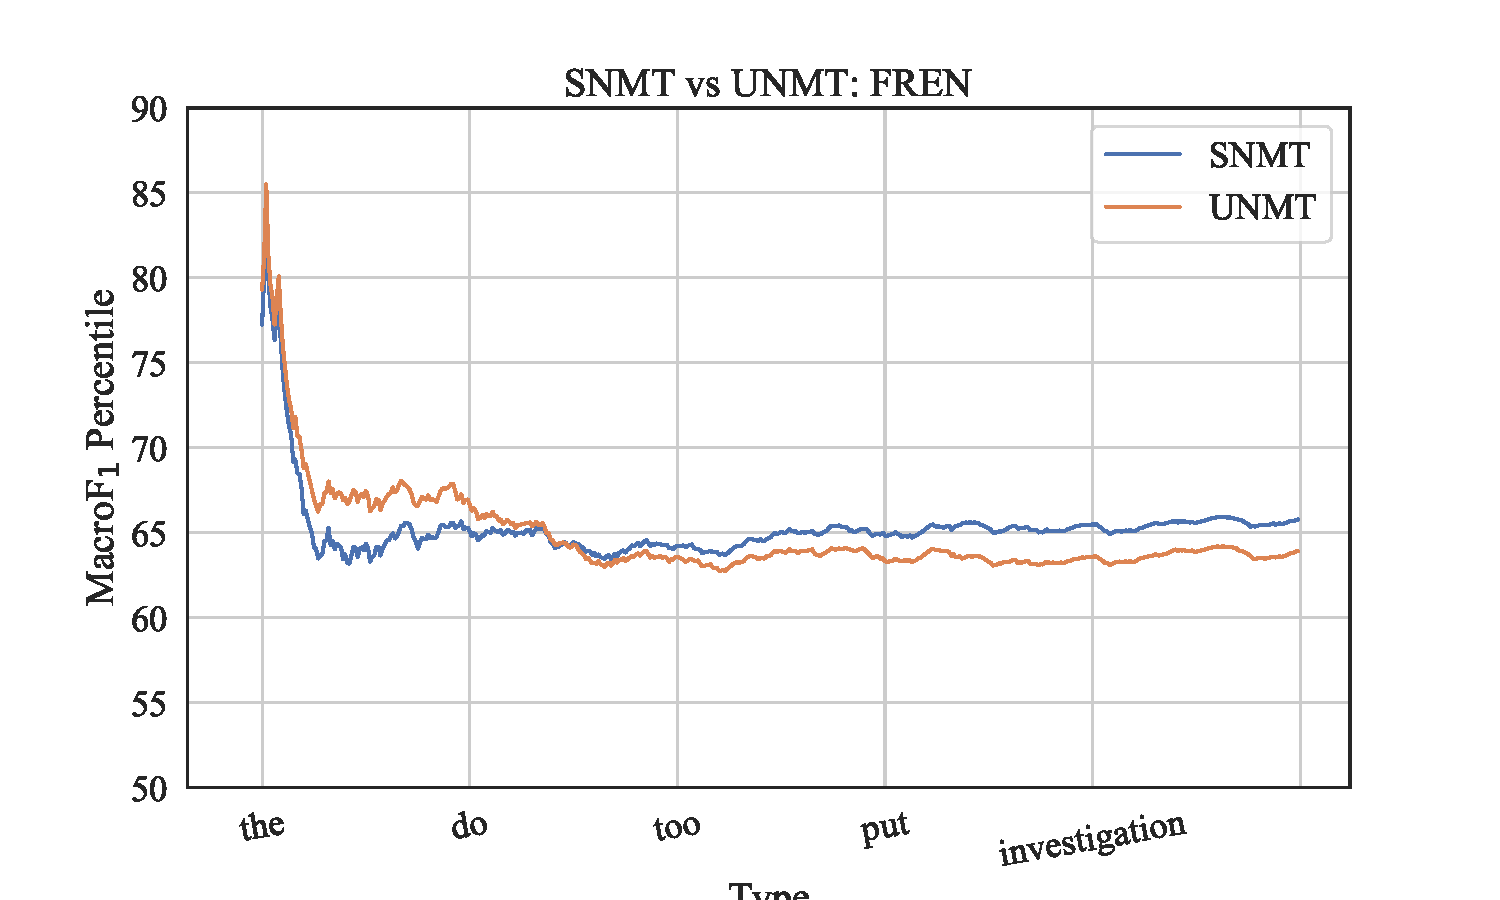
\includegraphics[width=\linewidth,trim={13mm 5mm 25mm 10mm},clip]{img/s_unmt-fren-maf1.pdf}
    \end{subfigure}
    \hfill 
    \begin{subfigure}[b]{0.9\linewidth}
    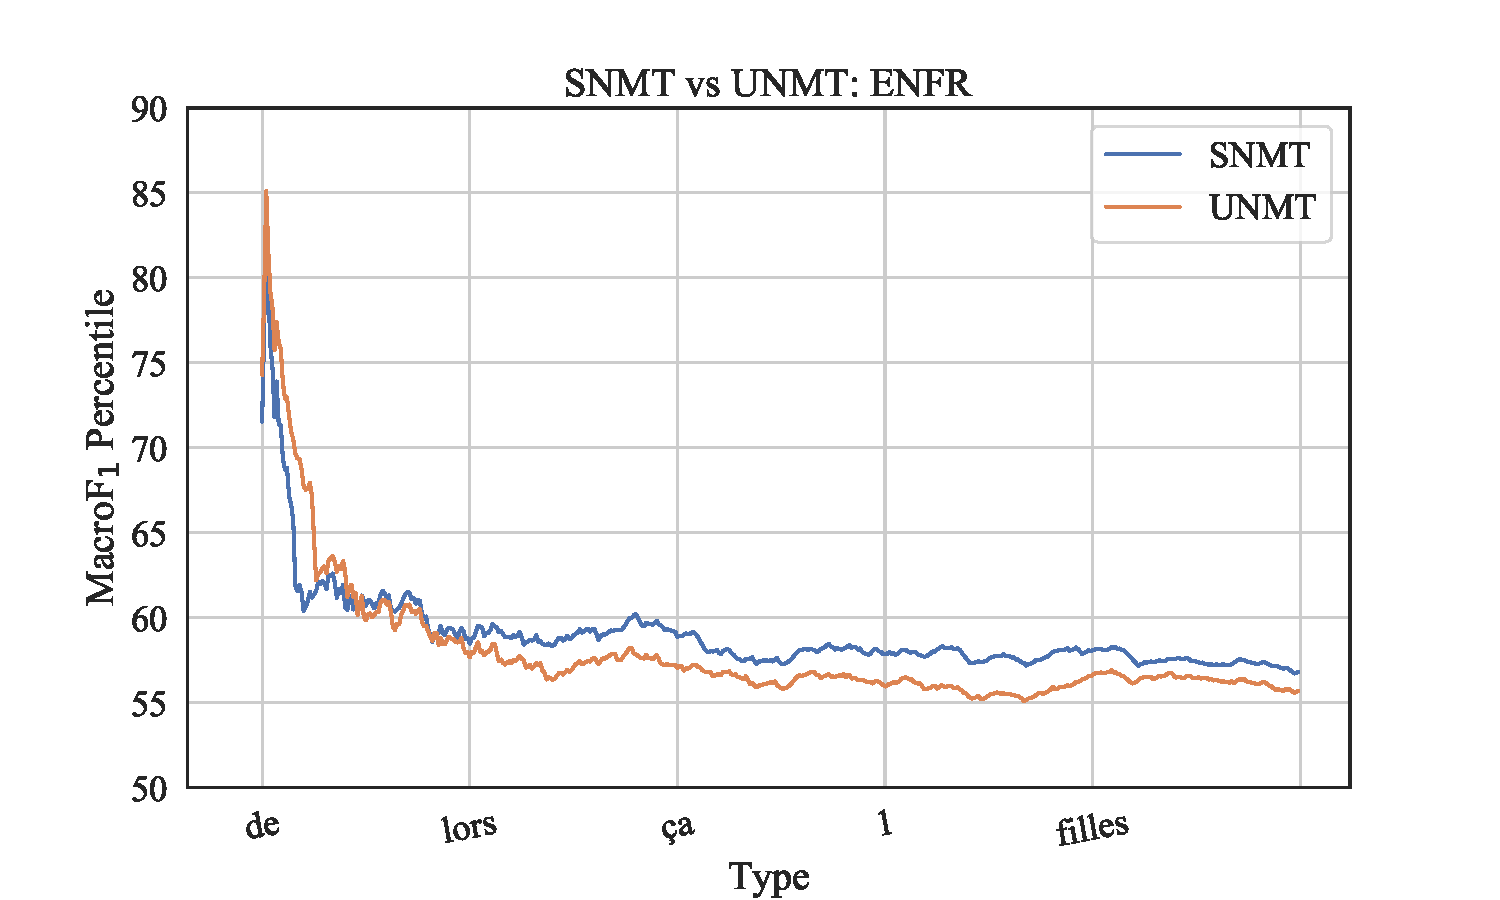
\includegraphics[width=\linewidth,trim={13mm 7mm 25mm 10mm},clip]{img/s_unmt-enfr-maf1.pdf}
    \end{subfigure}
    
    \begin{subfigure}[b]{0.9\linewidth}
    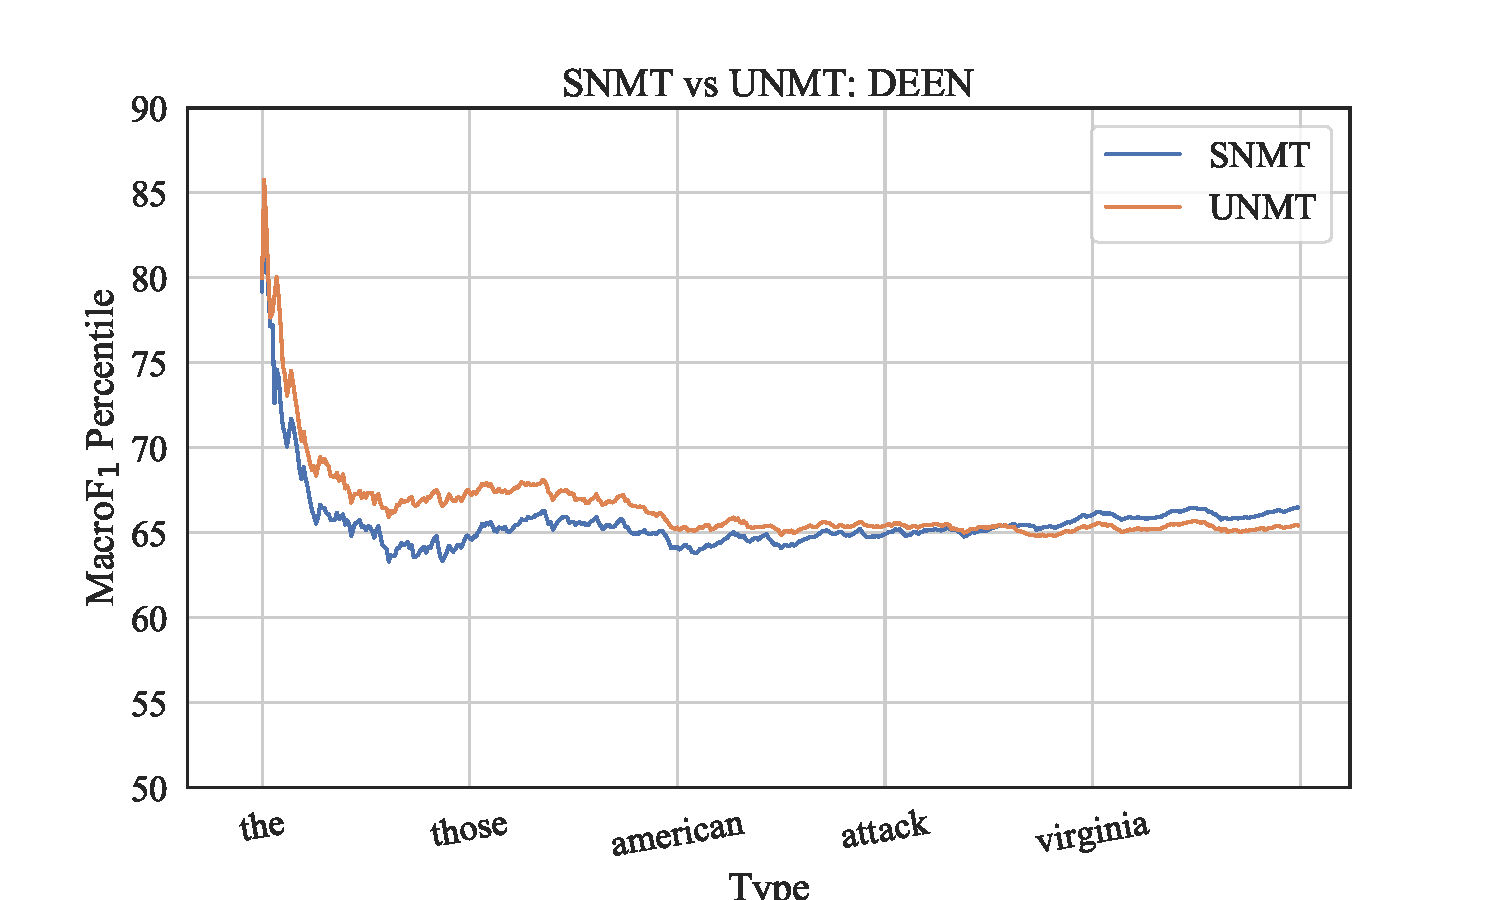
\includegraphics[width=\linewidth,trim={13mm 5mm 25mm 10mm},clip]{img/s_unmt-deen-maf1.pdf}
    \end{subfigure}
    \hfill 
    \begin{subfigure}[b]{0.9\linewidth}
    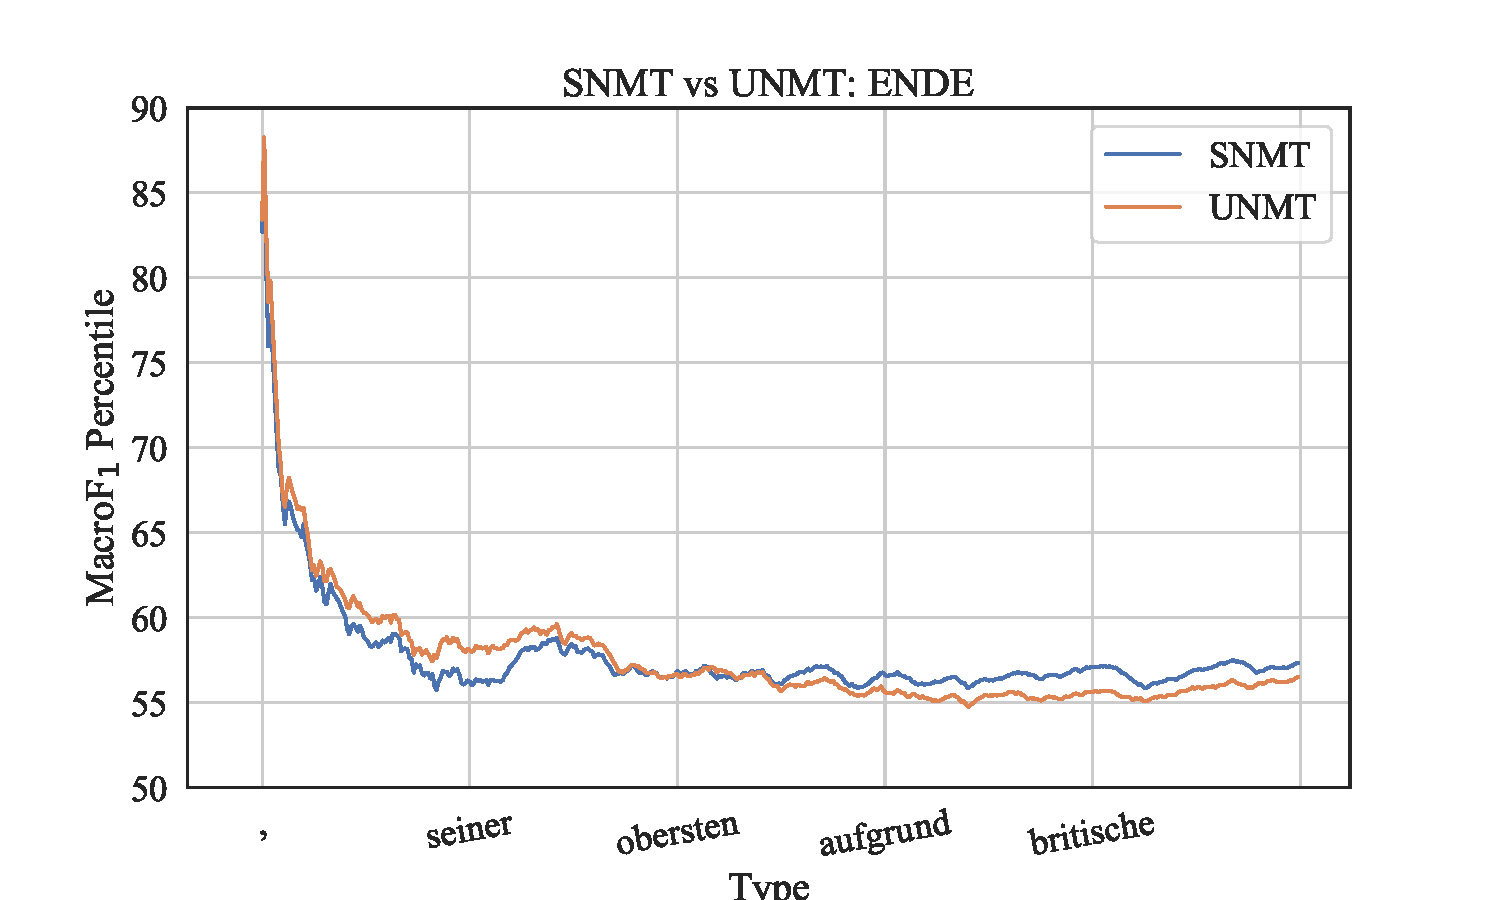
\includegraphics[width=\linewidth,trim={13mm 7mm 25mm 10mm},clip]{img/s_unmt-ende-maf1.pdf}
    \end{subfigure}
    
    \begin{subfigure}[b]{0.9\linewidth}
    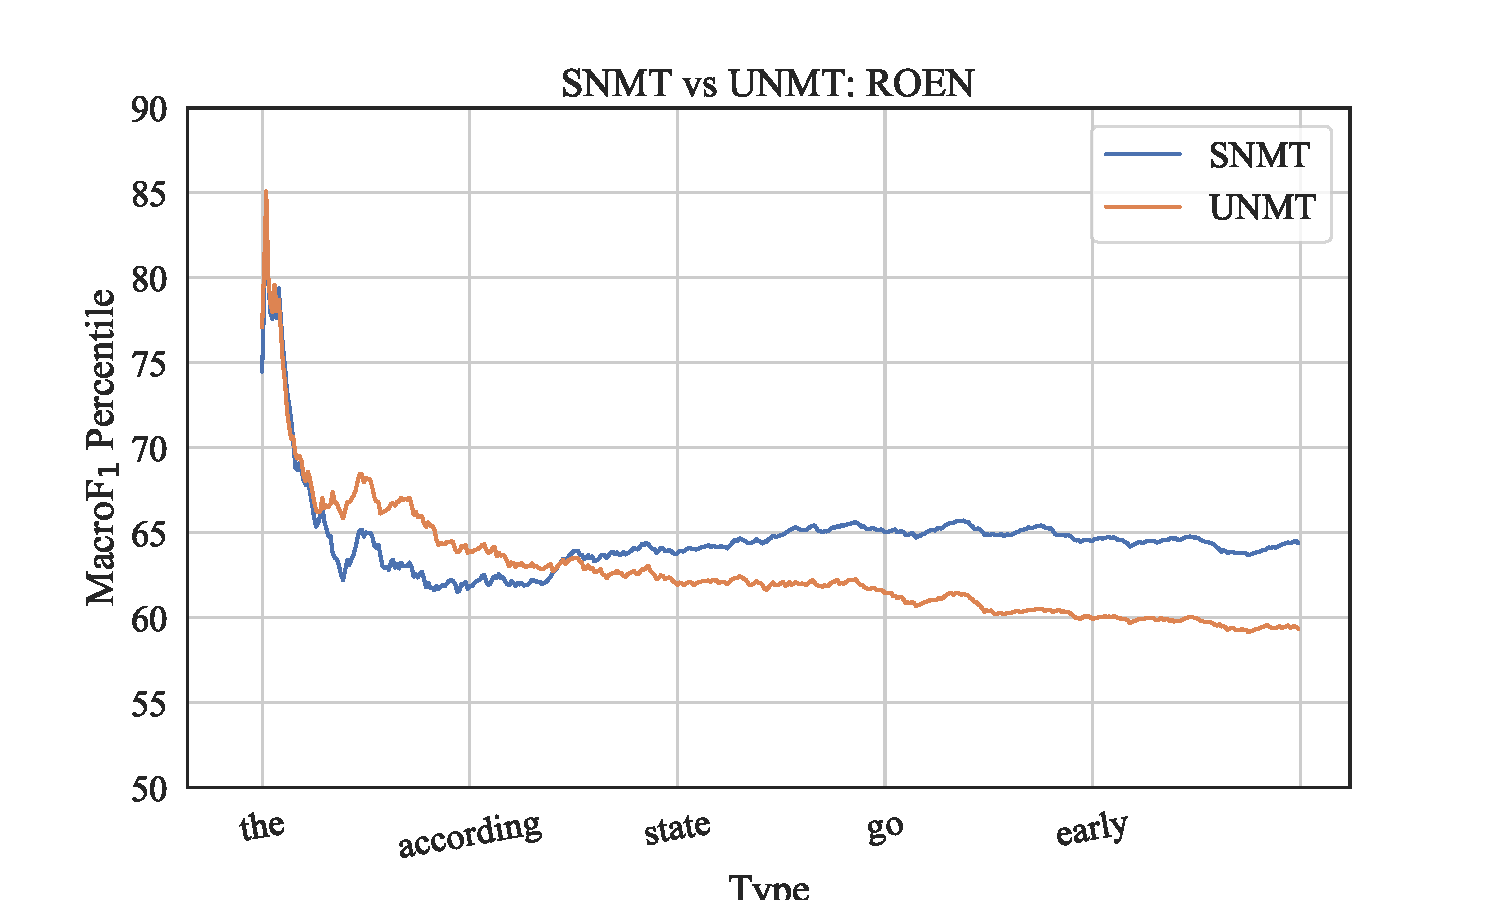
\includegraphics[width=\linewidth,trim={13mm 5mm 25mm 10mm},clip]{img/s_unmt-roen-maf1.pdf}
    \end{subfigure}
\caption{SNMT vs UNMT \maf1 on the most frequent 500 types.
UNMT outperforms SNMT on frequent types that are weighed heavily by \bleu\, however, SNMT is generally better than UNMT on rare types; hence, SNMT has a higher \maf1. 
}
\label{fig:snmt_vs_unmt}
\end{figure}


% \begin{figure}[ht]
%     \centering
%     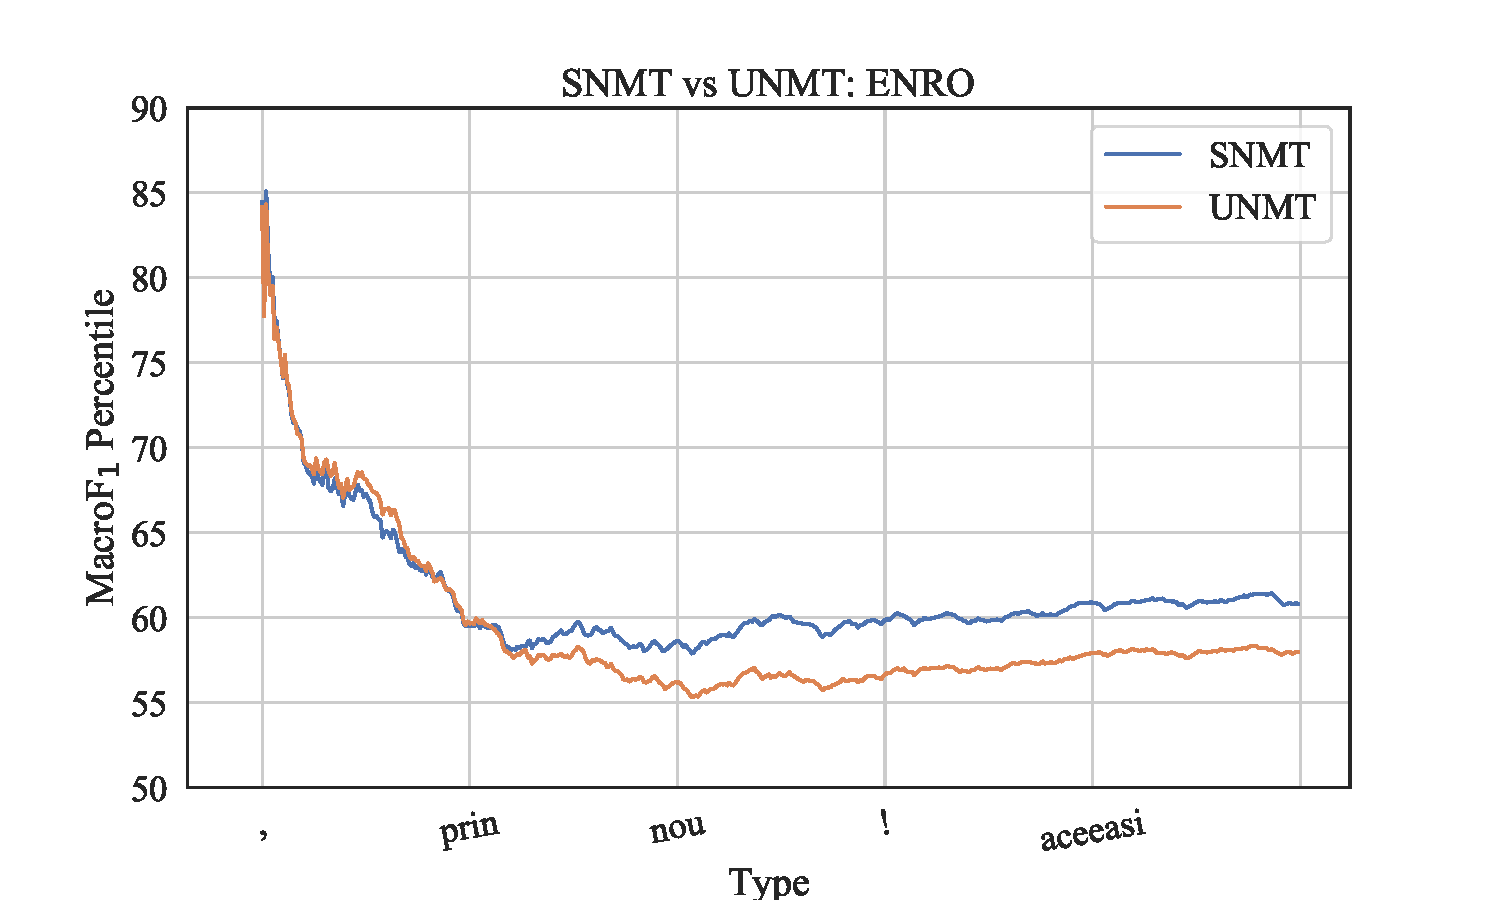
\includegraphics[width=\linewidth,trim={13mm 7mm 25mm 10mm},clip]{img/s_unmt-enro-maf1.pdf}
%     \label{fig:snmt_vs_unmt_rest}
%     \caption{(Continued from Figure~\ref{fig:snmt_vs_unmt}) Visualization of \maf1 between SNMT and UNMT .  }
% \end{figure}


The UNMT models follow XLM's standard architecture and are trained with 5 million monolingual sentences for each language using vocabulary size of 60,000. 
% using code base from \citet{rtg-xt20}
We train SNMT models for EN-DE and select models with the most similar (or a slightly lower) BLEU as their UNMT counterparts on newstest2019. The DE-EN model selected is trained with 1 million sentences of parallel data and a vocabulary size of 64,000, and the EN-DE model selected is trained with 250,000 sentences of parallel data and a vocabulary size of 48,000. For English$\leftrightarrow$French and English$\leftrightarrow$Romanian, we select SNMT models from submitted systems to WMT shared tasks that have similar or slightly lower BLEU scores to corresponding UNMT models, based on newstest2014 for English$\leftrightarrow$French and newstest2016 for English$\leftrightarrow$Romanian. 

Figure~\ref{fig:snmt_vs_unmt}, which is a visualization of \maf1 for SNMT and UNMT models,  shows that UNMT is generally better than SNMT on frequent types, however, SNMT outperforms UNMT on the rest indicating a cross over point in \maf1 curves. 
Since \maf1 assigns relatively higher weights to infrequent types than in \bleu{}, SNMT scores higher \maf1 than UNMT while both have the same \bleu{}, as reported in Table~\ref{tab:unmt_vs_snmt}.

The complete comparison of UNMT vs SNMT in different languages is in Table~\ref{tab:unmt_vs_snmt2}. A manual analysis of the ten sentences with the largest magnitude favoritism according to \maf1 and \bleu\ in the FR-EN and RO-EN test sets is in Table~\ref{tab:snmt_better_mf1_fren} and Table~\ref{tab:snmt_better_mf1_roen}. The complete texts of these sentences, their reference translations, and the system translations (including DE-EN mentioned in Sec~\ref{sec:unmt}), are shown in Tables \ref{tab:maf1-top-10}, \ref{tab:bleu-top-10}, \ref{tab:maf1-top-10-fren}, \ref{tab:bleu-top-10-fren}, \ref{tab:maf1-top-10-roen}, and \ref{tab:bleu-top-10-roen}. 

% Qualitative examples for analyzing with $\Delta Rank(i; h_S, h_U)$ are shown in Table~\ref{tab:diff_mf1_bleu}.

% \subsection{Qualitative Analysis of Supervised and Unsupervised NMT}
\label{app:extraqual}

\begin{table*}[ht!]
    \centering
    \footnotesize
    \begin{tabular}{r @{\hspace{2mm}} l @{\hspace{2mm}} p{0.34\linewidth} | r @{\hspace{2mm}} l @{\hspace{2mm}} p{0.34\linewidth} }
 $\delta_{\maf1}$ & Fav & Analysis 
    & $\delta_{\bleu}$ & Fav   & Analysis \\ \hline \hline
 
 .044   & S  & S: synonym; U: \textit{untranslation}, synonym 
    &  -.026   & U  & U: synonym; S: \textit{omitted adv}, word order \\
 
 -.038   & U  & U: no issues; S: synonym 
    & .025   & S  & S: no issues; U: \textit{determiner}, word order \\ 
 
 .035  & S  & S: synonym; U: \textit{untranslation}, synonym    
    & .024   & S  & S: no issues; U: \textit{repetition}, form  \\

 -.034   & U  & U: no issues; S: synonym; word\_order
    & .021   & S  & S: \textit{verb}, synonym; U: \textit{untranslation}, \textit{noun}, \textit{time}, synonym \\ 
 
 -.034  & U  & U: synonym; S: \textit{word order}, verb\_ref  
  & .021  & S  & S: synonym; U: synonym  \\
 
 -.033   & U  & U: no issues; S: synonym
  &  -.021  & U  & U: \textit{omitted NER}; S: synonym, word order  \\
 
 .033   & S  & S: word order; U: \textit{untranslation}, NER, word order 
  & -.021  & U  & U: \textit{untranslation}; S: \textit{verb}, word order  \\
 
 .032  & S  & S: synonym; U: \textit{ number}, \textit{omitted noun}, \textit{untranslation}, \textit{verb} 
    & -.021  & U  & U: synonym; S: \textit{extra preposition}, synonym, word order \\
 
 .030  & S  &  S: \textit{adj}; U: \textit{untranslation}
  & .021  & S  & S: no issues; U: \textit{NER} \\
   
.030    & S & S: \textit{noun}, synonym; U: \textit{noun}, synonym  
  & -.020  & U  & U: synonym; S: synonym, word order 
\end{tabular}
\caption{Analysis of the ten FR-EN test set segments with the most favoritism in SNMT (S) or UNMT (U), according to $\maf1$ (left) and $\bleu$ (right). Fav is the favored system by metrics. Actual examples are shown in Appendix Tables~\ref{tab:maf1-top-10-fren} and \ref{tab:bleu-top-10-fren}.}
\label{tab:snmt_better_mf1_fren}
\end{table*}


\begin{table*}[ht!]
    \centering
    \footnotesize
    \begin{tabular}{r @{\hspace{2mm}} l @{\hspace{2mm}} p{0.34\linewidth} | r @{\hspace{2mm}} l @{\hspace{2mm}} p{0.34\linewidth} }
 $\delta_{\maf1}$ & Fav & Analysis 
    & $\delta_{\bleu}$ & Fav   & Analysis \\ \hline \hline
 
 .131   & S  & S: word order; U: \textit{repetition}, word order 
    &  .114   & S  & S: word order; U: \textit{repetition}, \textit{word order} \\
 
 .063   & S  & S: \textit{noun}, word order; U: \textit{repetition}, \textit{untranslation}, \textit{noun} 
    & .089   & S  & S: no issues; U: \textit{omitted noun}, \textit{omitted time}, \textit{NER} \\ 
 
 .062  & S  & S: \textit{extra}, \textit{untranslation}; U: \textit{untranslation}, \textit{copy}    
    & -.072   & U  & U: \textit{country}, \textit{untranslation}; S: \textit{noun}, \textit{word order}  \\

 -.052   & U  & U: \textit{untranslation x 3}, synonym; S: \textit{untranslation}, synonym
    & -.045   & U  & U: synonym; S: synonym, word order\\ 
 
 -.052  & U  & U: \textit{untranslation}, \textit{NER}, synonym; S: \textit{NER}, synonym 
  & -.041  & U  & U: \textit{untranslation}; S: \textit{word order}, \textit{subject}  \\
 
 -.052   & U  & U: \textit{extra}; S: \textit{untranslation}
  &  -.040  & U  & U: no issues; S: \textit{number}, \textit{omitted preposition}  \\
 
 -.050   & U  & U: \textit{adv}; S: \textit{incoherent}, \textit{adv}
  & .039  & S & S: \textit{extra}, \textit{untranslation}; U: \textit{untranslation}, \textit{copy}  \\
 
 -.050  & U  & U: \textit{active/passive voice}, \textit{name}; S: \textit{ name} 
    & .036  & S  & S: no issues; U: \textit{extra verb} \\
 
 -.049  & U  &  U: \textit{untranslation}; S: \textit{untranslation}, \textit{word order}
  & -.035  & U  & U: \textit{repetition}, \textit{untranslation}, S: \textit{verb}, synonym, word order \\
   
.048    & S & S: no issues; U: \textit{NER}
  & .034  & S  & S: synonym; U: \textit{untranslation}
\end{tabular}
\caption{Analysis of the ten RO-EN test set segments with the most favoritism in SNMT (S) or UNMT (U), according to $\maf1$ (left) and $\bleu$ (right). Fav is the favored system by metrics. Actual examples are shown in Appendix Tables~\ref{tab:maf1-top-10-roen} and \ref{tab:bleu-top-10-roen}.}
\label{tab:snmt_better_mf1_roen}
\end{table*}

% \begin{table*}[ht]
%     \centering
%     \resizebox{\textwidth}{!}{%
%     \begin{tabular}{l|l}
    
% 3$^{rd}$ & $\delta_{\maf1} (x; S, U)$: 0.014, $\delta_{\bleu} (x; S, U)$: -0.025, $\delta_{BLEURT} (x; S, U)$: 0.898 \\\hline
% Src & Zu den Finanzierungsmöglichkeiten für Langzeitpflege gehören eine traditionelle \colorbox{pink}{Pflegeversicherung}, eine hybride \\
% &kapitalbindende Lebensversicherung zur Abdeckung dieser Ausgaben oder eine Selbstversicherung mit dem eigenen \\
% &Vermögen – solange Sie das Geld dafür haben.\\\hline
% Ref & Your funding choices for long-term care can include a traditional long-term \colorbox{pink}{care insurance policy}, a hybrid cash-value \\
% &life insurance policy to help cover these expenses or self-insuring with your own wealth - as long as you have the money.\\\hline
% SNMT& Financing opportunities for long-term care include traditional \colorbox{pink}{care insurance}, hybrid capital-binding life insurance to \\
% &cover this spending, or self-insurance with your own assets – as long as you have the money for it.,,,,,,,,,,,,,,,,, etc.\\\hline
% UNMT& Among the financing options for long-term care are a traditional \colorbox{pink}{Pflegeversicherung}, a hyper-fat equity binoculars to \\
% &cover these expenses or a self-fund with your own wealth - as long as you have the money for it.\\\hline
% Problems&SNMT: synonym, punctuation, \textit{omit\_adj}. UNMT: synonym, \colorbox{pink}{\textit{untranslation}}, \textit{wrong\_adj}, \textit{wrong\_noun}.\\\hline\hline

% 4$^{th}$ & $\delta_{\maf1} (x; S, U)$: 0.037, $\delta_{\bleu} (x; S, U)$: -0.011, $\delta_{BLEURT} (x; S, U)$: 0.961 \\\hline
% Src & Trotzdem war der Ton von Ri's Rede dramatisch anders als letztes Jahr, als er es der U.N. berichtete. Die Generalversa-\\
% &mmlung, \colorbox{yellow}{die das US-Festland mit Nordkoreas Raketen ins Visier nahm, war unvermeidlich, nachdem ``Mr. Evil President"} \\
% &\colorbox{yellow}{Trump Kim als ``Raketenmann" auf einer Selbstmordmission bezeichnete.}\\\hline

% Ref & Even so, the tone of Ri's speech was dramatically different from last year, when he told the U.N. General Assembly \colorbox{yellow}{that} \\
% &\colorbox{yellow}{targeting the U.S. mainland with North Korea's rockets was inevitable after ``Mr Evil President" Trump called Kim a} \\
% &\colorbox{yellow}{``rocket man" on a suicide mission.}\\\hline

% SNMT& However, the tone of Ri's speech was dramatically different from last year when he reported it to the U.N., and the \\
% &General Assembly, \colorbox{yellow}{targeting the US mainland with North Korea ' s missiles, was inevitable after ``Mr. Evil President "} \\
% &\colorbox{yellow}{Trump called Kim a`` missile man " on a suicide mission.}\\\hline

% UNMT& Nonetheless, the tone of Ri's speech was dramatically different from last year when he reported it to the U.N. General \\
% &Assembly. \colorbox{yellow}{ }\\\hline

% Problems&SNMT: punctuation, synonym. UNMT: \colorbox{yellow}{\textit{truncation}}.\\


%     \end{tabular}
%     }
%     \caption{Cases to show different qualities \maf1 and \bleu value. a) The 3rd ranked sentence has untranslation in UNMT translation that is disfavored by \maf1 but not \bleu. b) The 4th ranked sentence has the whole second half of the sentence truncated in UNMT's translation, and \maf1 prefers SNMT's translation while BLEU still prefers UNMT. }
%     \label{tab:diff_mf1_bleu}
% \end{table*}

% {r @{\hspace{2mm}} l @{\hspace{2mm}} p{0.70\linewidth}}


\begin{table*}[ht]
%\scriptsize
\centering
\fontsize{8}{8}
\selectfont
%\scalebox{0.66}{
\begin{tabular}{r @{\hspace{2mm}} p{0.21\linewidth}p{0.2\linewidth}p{0.2\linewidth}p{0.2\linewidth}}
 $\delta_{\maf1}$&Source & Reference & SNMT & UNMT \\\hline\hline
.071 & Es wird davon ausgegangen, dass sie über eine leistungsstarke Kanone, eine Reihe von Flugabwehr- und Schiffsabwehrraketen sowie einige Stealth-Technologien verfügen, wie z. B. reduzierte Radar-, Infrarot- und akustische Signaturen.                                                                                                                                                         & It is understood they will feature a powerful cannon, an array of anti-aircraft and anti-ship missiles as well as some stealth technologies, such as reduced radar, infrared and acoustic signatures.                                                                                                                & It is assumed that they have a powerful cannon, a series of anti-aircraft and anti-ship missiles, as well as some steam technologies, such as reduced radar, infrared and acoustic signatures.                                                                                      & It is understood they have a powerful canon, a number of fluke and ship fire systems and some stealth-controlled technologies, such as reduced radar, infrarot and akustic signposts.                                                                                                    \\\hline
.064&Eine Gruppe maskierter Pro-Separatisten, die von der Bereitschaftspolizei zurückgehalten wurden, bewarfen sie mit Eiern und schleuderte Pulverfarbe und erzeugte in den Straßen, die normalerweise von Touristen überfüllt waren, dunkle Staubwolken.                                                                                                                                           & A group of masked pro-separatists held back by riot police pelted them with eggs and hurled powder paint, creating dark clouds of dust in streets that would usually be thronged with tourists.                                                                                                                      & A group of masked pro-separatists held hostage by the riot police brought them to eggs and ignited powder paint and produced dark clouds in the streets that were usually crowded by tourists.                                                                                      & A group of masked pro-independence separforces, who were kept away by the Bereitschaftpolice, beheaded them with evocative paint and poured pulverforce paint and created dark Staubations in the streets normally clogged by tourists.                                                  \\\hline
-.055&Il faut bien le faire.                                                                                                                                                                                                                                                                                                                                                                          & Il faut bien le faire.                                                                                                                                                                                                                                                                                               & La gentillesse du personnel et la disponibil.                                                                                                                                                                                                                                       & Il faut bien faire.                                                                                                                                                                                                                                                                      \\\hline
.052&In einem Abschnitt gibt es ein Bild eines Schlafsaals, in dem die Studenten auf Kaffeetassen, Vorhänge, Trainer und Bücher klicken, um über die Auswirkungen von Koffein und Licht informiert zu werden und darüber, wie sich die sportliche Leistung durch Schlafmangel und die Bedeutung einer Schlafenszeitroutine beeinflusst.                                                              & In one section there is an image of a dorm room, where students click on coffee cups, curtains, trainers and books to be told about the effects of caffeine and light and how athletic performance is impacted by sleep deficiency, and the importance of a bedtime routine.                                         & In a section there is an image of a bedroom where students click on coffee cups, curtains, trainers, and books to be informed about the effects of caffeine and light, and about how sporting performance is affected by lack of sleep and the importance of sleeping time routine. & In one section, there is a picture of a sleeping sauna where students click on coffee cups, forecourts, coaches and books to be educated about the impact of Koffein and light and about how athletic performance is influenced by sleep loss and the importance of a sleep day routine. \\\hline
-.045&Nickelbergbau ist auch in der Provinz wichtig, wird aber hauptsächlich in Morowali betrieben, an der gegenüberliegenden Küste von Sulawesi.                                                                                                                                                                                                                                                     & Nickel mining is also important in the province, but is mostly concentrated in Morowali, on the opposite coast of Sulawesi.                                                                                                                                                                                          & Nickelergbau is also important in the province, but is mainly operated in Morewali, on the opposite coast of Sulawesi.                                                                                                                                                              & Nickel mining is also important in the province, but is mostly operated in Morowali, on the opposite coast of Sulawesi.                                                                                                                                                                  \\\hline
.044&Vor 32 Jahren schloss ich mich als Schüler, wegen der Vernachlässigung der Thatcher-Regierung, Labour an. Diese Vernachlässigung hatte dazu geführt, dass mein Klassenzimmer buchstäblich zusammengebrochen war. Infolgedessen habe ich versucht, mich für bessere öffentliche Dienstleistungen für diejenigen einzusetzen, die sie am meisten brauchen. Egal ob als Gemeinderat oder Minister. & Ever since I joined Labour 32 years ago as a school pupil, provoked by the Thatcher government's neglect that had left my comprehensive school classroom literally falling down, I've sought to champion better public services for those who need them most - whether as a local councillor or government minister. & 32 years ago, I joined Labour as a student because of the neglect of the Thatcher government, which had led to my classroom literally collapsed, and as a result I tried to promote better public services for those who need it most, whether as a local council or ministers.     & Last 32 years ago, as a student, because of the disdain for the Thatcher-era government, Labour joined Labour.                                                                                                                                                                           \\\hline
.044&UN-Gesandter Staffan de Mistura hofft, bald die ersten Treffen eines neuen Ausschusses aus Regierungs- und Oppositionsmitgliedern einzuberufen, um eine Nachkriegsverfassung für Syrien zu entwerfen und den Weg zu Wahlen zu ebnen.                                                                                                                                                            & UN envoy Staffan de Mistura is hoping to soon convene the first meetings of a new committee comprised of government and opposition members to draft a post-war constitution for Syria and pave the way to elections.                                                                                                 & UN envoy Staffan de Mistura hopes to convene soon the first meetings of a new committee of government and opposition members to draw up a post-war constitution for Syria and pave the way for elections.                                                                           & U.N. Secretary General Staffan de Mistura hopes to soon join the first meetings of a new committee of government and opposition leaders to design a Nachkriegsrewrite for Syria and clear the path to elections.                                                                         \\\hline
.043&CBS hatte 3,1 Millionen, NBC 2,94 Millionen, MSNBC 2,89 Millionen und CNN 2,52 Millionen, so Nielsen.                                                                                                                                                                                                                                                                                           & CBS had 3.1 million, NBC had 2.94 million, MSNBC had 2.89 million and CNN had 2.52 million, Nielsen said.                                                                                                                                                                                                            & CBS had 3.1 million, NBC 2.94 million, MSNBC 2.89 million and CNN 2.52 million, says Nielsen.                                                                                                                                                                                       & CBS had 3.8 million, NBC 3.94 million, MSNBC 3.89 million and CNN 3.52 million, Nielsen said.                                                                                                                                                                                            \\\hline
-.041&Den Rangers gelangen nur zwei Schüsse in der ersten Hälfte, aber der ehemalige Ibrox-Torhüter Liam Kelly war kaum von Lassana Coulibalys Kopfsprung und dem Treffer eines bisslosen Ovie Ejaria aus der Ruhe zu bringen.                                                                                                                                                                        & Rangers managed just two first-half shots on target but former Ibrox goalkeeper Liam Kelly was barely troubled by Lassana Coulibaly's header and a tame Ovie Ejaria strike.                                                                                                                                          & The Ranners only reach two shots in the first half, but the former Ibrox-Torkeeper Liam Kelly was hardly the head of Lassanna Coulibys and the hit of a bissloze Ovi Ejaria.                                                                                                        & The Rangers managed only two shots in the first half but former Ibrox goalkeeper Liam Kelly was unlikely to be helped by Lassana Coulibaly's headfirst tackle and the goal of a bisected Ovie Ejaria.                                                                                    \\\hline
.041&Liverpool tritt am MIttwoch um 15.00 Uhr im Stadio San Paolo in Neapel, Italien, gegen Napoli an.                                                                                                                                                                                                                                                                                               & Liverpool battles Napoli in the group stage of the Champions League at 3 p.m. on Wednesday at Stadio San Paolo in Naples, Italy.                                                                                                                                                                                     & Liverpool will take place at 3 p.m. at the Stadio San Paolo in Naples, Italy, against Napoli.                                                                                                                                                                                       & Liverpool v Napoli at the MItch Stadium at 15.00 pm in Neapel, Italy, on MItch.
\end{tabular}
%}
\caption{Top 10 segments by $|\delta_{\maf1}(i, h_S, h_U)|$ on DE-EN.}
\label{tab:maf1-top-10}
\end{table*}

%%% extra extra stuff 
%\clearpage
%
%%%%%%%%%%%%%%%%%%%%%%%%%%%%%
\tg{Anything below here is saved for future use (in thesis). these are not going into paper. }
%%%%%%%%%%%%%%%%%%%%%%%%%%%%

\section{BLEU and CHRF Definition}
\label{sec:bleu-def}

BLEU~\cite{papineni-etal-2002-bleu} has become the de-facto automatic evaluation for MT.
Except a word tokenizer, BLEU does not use any other linguistic resources such as parsers, synonyms etc. 
In addition, BLEU is computationally efficient; works reasonably well on all languages with word boundaries, and has advanced MT research for almost two decades now.


A key component of BLEU is $$\text{ModifiedPrecision} = \frac{\text{TotalMatch}}{\text{TotalPredictions}}$$

On a test corpus of $m$ pairs $$ \mathcal{T} = \{ (h^{(i)}, y^{(i)}) | i = 1,2,3...m \} $$ where $h$ is hypothesis, and $y$ is reference aka gold translation.

$$match_w = min \{ count(w, h), count(w, y) \}$$ 

 ModifiedPrecsion, $P_n$ defined for n-grams, $n=\{1, 2, 3, 4\}$ as
 $$ P_n = \frac{\sum_{(h, y) \in \mathcal{T}}  \sum_{k \in h} match_{k} (h, y) }{ \sum_{k' \in \mathcal{T}}  \sum_{k' \in h'} count(k, h) }$$  
 where $k$ is an n-gram in sentence $h$ or $y$.

Does not make any distinction between word types. 
Opinion: Should this be called $ModifiedAccuracy$ instead of $ModifiedPrecision$ ?

BLEU reduce the n-gram precisions $P_1, P_2, P_3, P_4$ using geometric mean, as:
$$P = \sqrt[4]{P_1 \cdot P_2 \cdot P_3 \cdot P_4} = exp(\frac{1}{4}\sum_{n=1}^4  \log P_n )$$

Further, a possible generalization was proposed as:  $$P= exp(\sum_{n=1}^4 w_n \log P_n ) \text{ such that } \sum_{n=1}^4 w_n = 1$$
However, such generalization is rarely used in practice as weights $w_1, w_2, w_3, w_4$ are subjective to corpora. 
Hence, in practice, equal weights  are assigned to all the modified precisions of n-gram orders leading to \textit{macro or unweighted} geometric mean.

Lastly, to compensate the absence of recall measure, a term named brevity penalty, $BP$, is used a scaler: 
$$ BLEU = BP \cdot P = BP \cdot exp(\frac{1}{4}\sum_{n=1}^4  \log P_n ) $$
The scaler $BP$ is computed such that it penalizes the short translation that may arise due to poor recall.
Let $H$ be system hypotheses length, $R$ be references length. 
$$ BP = \begin{cases} 
  1                    & H > R \\
 e^{(1 - \frac{R}{H})} & H \le R 
 \end{cases}  = min \{1,  e^{(1 - \frac{R}{H})}\} $$

BLEU was originally devised to work with multiple references, however nowadays use of multiple references are rare. 



\subsection{\chr{F}{}1 and \chr{F}{}3}

\citet{popovic-2015-chrf} extend the idea of (modified-)precision of word n-grams of \bleu\ to characters (\chr{P}{}) n-grams, but unlike \bleu\ they also consider (modified-)recall (\chr{R}{n}) to compute F1 measure (\chr{F}{n} as harmonic mean of \chr{P}{n} and \chr{R}{n}, with a $\beta$ to weight toward recall.
They did not do an exhaustive search for values of $N$ and $\beta$: they consider $N=6$, i.e. up to 6-grams with $\beta=1$ and $\beta=3$.

$$\chrx{F}\beta = \frac{1}{N} \sum_{n=1}^{N}(1 + \beta^2) \frac{\chrx{P}_n \cdot \chrx{R}_n}{ \beta^2 \cdot \chrx{P}_n + \chrx{R}_n}$$

Even though the \chr{F}{}1 and \chr{F}{}3 compute F1 measure similar to our work, note that the \chr{P}{n} \chr{R}{n} are inherently micro-averaged by n-gram frequency as in \bleu \footnote{The implementation detail is not provided in \cite{popovic-2015-chrf}, but verified in the implementation of SacreBLEU-\chr{F}{} \url{https://github.com/mjpost/sacrebleu} (accessed July 2020) }.




\section{MT Autoeval Methods}
\begin{comment}

\begin{table}[ht]
\footnotesize
\begin{tabular}{ll}
 \textbf{Method}                            & \textbf{Category} \\
  \bleu \cite{papineni-etal-2002-bleu}       & Token-based   \\
  NIST \cite{nist2002}                      & Token-based   \\  
  TER  \cite{snover2006TER}                 & Token-based    \\      
  METEOR \cite{banerjee-lavie-2005-meteor}  & Resource-based? \\  
  %RIBES \cite{isozaki-etal-2010-autoeval}   & ?           \\  
  HyTER \cite{dreyer-marcu-2012-hyter}      & Resource-based \\
  BEER \cite{stanojevic-simaan-2014-beer}   & Model-based  \\
  \chrf{} \cite{popovic-2015-chrf}             & Resource-free \\      
  ESIM \cite{mathur-etal-2019-ESIM}         & Model-based \\  
  YiSi \cite{lo-2019-yisi}                  & Model-based            \\
  BLEURT \cite{sellam-etal-2020-bleurt}     & Model-based \\ 
  % ZeroShotPP \cite{thompson2020paraphrase-eval} & Model-based \\
\end{tabular}
\caption{An overview of automatic evaluation methods. }
\label{tab:eval-measures}
\end{table}

\end{comment}

\section{Metrics categories} 
\begin{enumerate}
    \item \textit{Resource-light}: These methods do not rely on linguistic resources \textit{except a tokenizer}. We consider tokenizer as a basic linguistic resource that is relatively easier to obtain than others, and it may often be borrowed from other languages.  
    The primary example for this category is BLEU \cite{papineni-etal-2002-bleu}.
    Since the choice of tokenizer varies based on language, and introduces some looseness in matching, the scores across publications over a long time span are only comparable if and only if the tokenizer is guaranteed to be the same. 
    The MT community has circumvent this limitations by making a tokenizer as a standard tokenizer (eg: NIST 13a, international etc).
    Other examples: NIST \cite{doddington2002-nist}, TER \cite{snover2006TER}, 
    
    \item \textit{Resource-free}: These methods do not rely on any linguistic resources. 
    These are readily portable to all languages and domains, as there is no dependence on whatsoever, and the scores are readily comparable across the publications. This category is relatively newer and less explored. E.g. CHRF \cite{popovic-2015-chrf}
    
    \item \textit{Resource-dependent}: These methods rely on resources that are not readily available or harder to construct for most languages. 
    This constraint limits their application to only a few languages to which resources are available. 
    The scores are comparable across publications over the decades if the resources used are guaranteed to be the same. The community has not worked towards establishing the standards, hence these methods are not popular.
    E.g. METEOR \cite{banerjee-lavie-2005-meteor}, HyTER \cite{dreyer-marcu-2012-hyter}

    
    \item \textit{Model-dependent}: These methods use machine learned model to predict the human judgements. 

    The core principle behind these methods is that they either use a pretrained neural model or had engineered features, which are then used by a regressor model to estimate human judgement scores.
    Such pretrained models are easier to obtain than the linguistic-resources of the previous category, hence this category is an active area of research.  
    Most of these methods use pretrained language models on target language to obtain a sentence representation for reference and hypothesis, and computes the match. e.g. ESIM \cite{mathur-etal-2019-ESIM}, YiSi \cite{lo-2019-yisi}, RUSE, BERTScore, BLEURT
    
    However, there are some \textit{model-dependent} methods that do not use references. Instead, they compute translation quality scores by matching the hypothesis directly against source sentences with the help of a cross-lingual pretrained model. e.g. YiSi \cite{lo-2019-yisi},
    
    While these methods are an interesting research direction, we express our following concerns: 
    
\begin{enumerate}
    \item Hidden Biases: Presence of undesired hidden biases in machine learning models is a known phenomenon \tg{cite}. 
    A bias of our primary interest is a marginalization of rare and minority concepts that affect the generation of rare words\cite{gowda2020finding}. 
    Since the NMT model is already uninterpretable, when the evaluator is also uninterpretable, and if practitioners are asked with "why an output is assigned with so-and-so score", the explanation practitioners can provide is- "the evaluator model estimated it and we do not know why". 
    Such a faith on uninterpretable entities in evaluation is against the spirit of science.
    \tg{Citation from biases literature}
    
    \item Instability: Pretrained models are approximations and these approximations improve over the time span, they do not offer the statistical stability over a long span of years to emerge as a de-facto. 
    
    % \item Paradox: a machine learned model evaluating a machine learned model; a robot testing a robot paradox (\tg{citation and a formal name}). 
\end{enumerate}

\end{enumerate}

\subsection{BLEU criticism}
In this work, we emphasize and address these two shortcomings of BLEU:
\begin{enumerate}
\item BLEU is based on modified-precision of n-grams which is performance is implicitly weighted by frequency of n-grams (i.e micro-averaged).
 The rare n-grams have lesser importance than the frequent n-grams in BLEU metric. 
 However, the reality is contrary: rare words carry more \textit{information}\footnote{as in information theory} than frequent words.
 To illustrate this, consider the below two sentences where some words are missing due to poor recall from a model, which of these can be interpreted?\\
X: \rule{5mm}{0.15mm} of U.S. \rule{5mm}{0.15mm} deaths are linked to nursing homes .\\
Y: 43\% \rule{5mm}{0.15mm} U.S. Coronavirus deaths are linked \rule{5mm}{0.15mm} nursing homes .\\

\item BLEU does not provide performance breakdown per n-gram types. A detailed breakdown such as precision, recall and F-measure of n-grams are useful in practice to improve the model performance by including more training examples to the n-grams that have poorer performance.
\end{enumerate}


\section{UNMT and SNMT}
Table~\ref{tab:snmt_better_bleu} and Table~\ref{tab:unmt_better_bleu} show the top 10 sentences when BLEU favors SNMT and UNMT respectively.

\begin{table*}[t]
    \centering
    \footnotesize
    % \scalebox{0.8}{%
    \begin{tabular}{ l l l c c }
    
       & SNMT & UNMT & $\beneficial{S}{U}{MacroF1}$ & $\beneficial{S}{U}{BLEU}$ \\ 
$1^{st}$ & \_word\_order    &	\_word\_order, \textbf{untranslation}, \textbf{wrong\_end} & 1.99E-02 & 4.76E-02 \\
$2^{nd}$ & \_diff\_spelling &	\_synonym, \_word\_order, \_punctuation&7.56E-03& 4.61E-02 \\
$3^{rd}$ & \_extra\_det     &	\_synophrase, \_synonym, \textbf{number}, &2.95E-02& 4.39E-02 \\
       &               &\textbf{measure\_word}, \textbf{untranslation} & \\
$4^{th}$ & \_synonym&	\_synonym, \_punctuation, \_extra\_adv&1.19E-02& 4.22E-02\\
$5^{th}$ & \_word\_order, \_synonym, &	\_synonym, \textbf{wrong\_verb}, \textbf{punctuation}&5.51E-03& 2.86E-02\\
& \_punctuation&&\\
$6^{th}$ & \_synonym, \_word\_order&	\_synonym, \_word\_order, \_omit\_verb&1.03E-02& 2.70E-02\\
$7^{th}$ & \textbf{wrong\_active\_passive}, &	\_synonym, \textbf{wrong\_active\_passive}, &2.70E-02&2.58E-02\\
& \textbf{omit\_adv}, \textbf{repetition}&extra\_phrase, \textbf{wrong\_pronoun}, &\\
& & \textbf{wrong\_tense} & \\
$8^{th}$ & \_synonym, \_inflection&	\textbf{untranslation}, wrong\_noun&4.43E-02& 2.54E-02\\
$9^{th}$ & \_synonym &	\textbf{untranslation}, \textbf{wrong\_noun}&3.66E-02& 2.52E-02\\
$10^{th}$ & \_synonym&	\_synonym, \textbf{wrong\_noun}, \textbf{wrong\_verb}, &9.46E-03& 2.46E-02\\

    \end{tabular}%
    % }
    \caption{Problems for top 10 sentences such that $\beneficial{S}{U}{BLEU}$ favors SNMT over UNMT for De-En. }
    \label{tab:snmt_better_bleu}
\end{table*}


\begin{table*}[t]
    \centering
    % \scalebox{0.8}{%
    \footnotesize
    \begin{tabular}{lllcc}
    
 & SNMT  & UNMT & $\beneficial{S}{U}{MacroF1}$&$\beneficial{S}{U}{BLEU}$\\ 
$1^{st}$ &\textbf{wrong\_noun}, \textbf{wrong\_verb}	&&-8.84E-03&-3.88E-02\\
$2^{nd}$ &\_punctuation	&&-9.27E-04&-3.67E-02\\
$3^{rd}$ &\_symbol	&&-1.66E-02&-3.40E-02\\
$4^{th}$ &\textbf{wrong\_adj}, \textbf{wrong\_noun}	&&-1.56E-02&-3.22E-02\\
$5^{th}$ &\_tense, \textbf{word\_order}, \textbf{wrong\_meaning}, &	\textbf{untranslation}&-6.70E-03&-3.16E-02\\
&\textbf{wrong\_active\_passive} && \\
$6^{th}$ &\_word\_order, \_synonym, \textbf{extra\_conj}&	\textbf{untranslation}&-2.69E-03&-3.07E-02\\
$7^{th}$ &\_word\_order, \textbf{omit\_name}&	\textbf{untranslation}, \textbf{wrong\_noun}&-1.47E-02&-2.95E-02\\
$8^{th}$ &\_synonym, \textbf{wrong\_verb}, &	\textbf{time}, \textbf{untranslation}&-1.90E-02&-2.88E-02\\
&\textbf{wrong\_active\_passive} && \\
$9^{th}$ &\_word\_order, \textbf{wrong\_phrase}&&3.72E-04&-2.86E-02\\	
$10^{th}$ &\_punctuation, \textbf{wrong\_verb}&	\_synonym&-4.64E-03&-2.77E-02\\

    \end{tabular}%
    % }
    \caption{Problems for top 10 sentences such that $\beneficial{S}{U}{BLEU}$ favors UNMT over SNMT for De-En. }
    \label{tab:unmt_better_bleu}
\end{table*}


\begin{table*}[ht]
%\scalebox{0.63}{
\centering
\fontsize{7.8}{7.8}
\selectfont
\begin{tabular}{r @{\hspace{1mm}} p{0.25\linewidth}p{0.2\linewidth}p{0.2\linewidth}p{0.2\linewidth}}
 $\delta_{\bleu}$ & Source   & Reference& SNMT & UNMT  \\\hline\hline
.048  & In der letzten Woche wurden mittlere Konzentrationen in Küstennähe und auf offener See in Pinellas County gemeldet, geringe bis hohe Konzentrationen auf offener See in Hillsborough County, Hintergrund- bis hohe Konzentrationen in Manatee County, Hintergrund- bis hohe Konzentrationen in Küstennähe und auf offener See in Sarasota County, Hintergrund- bis mittlere Konzentrationen in Charlotte County, Hintergrund- bis hohe Konzentrationen in Küstennähe und auf hoher See in Lee County sowie geringe Konzentrationen in Collier County. & Medium concentrations in or offshore of Pinellas County have been reported in the past week, low to high concentrations offshore of Hillsborough County, background to high concentrations in Manatee County, background to high concentrations in or offshore of Sarasota County, background to medium concentrations in Charlotte County, background to high concentrations in or offshore of Lee County, and low concentrations in Collier County. & Last week, average concentrations were reported on the coast and open seas in Pinellas County, low to high levels at open sea in Hillsborough County, background to high concentrations in Mantee County, high concentrations in coastal and open seas in Sarsota County, background to medium concentrations in Charlotte County, background to high shore and high sea levels in Lee County, and low concentrations in Collier County. & In the last week, moderate to high Konzentrof lead in Küstas County were reported in Pinellas County, low to high Konzentrof lead levels on open water in Hillsborough County, Hintergrundto high levels in Manatee County, Hintergrundto high to high Konzentrin Küstas and on open water in Sarasota County and low Konzentrationen in Charlotte County, Hintergrundto high to high Konzentrin Küstennähe and on open water in Sarasota County. \\\hline
.046  & Moskau hat wiederholt betont, dass die 11-Milliarden-Dollar-Pipeline Nord Stream 2, die die bestehende Pipeline-Kapazität auf 110 Milliarden Kubikmeter verdoppeln soll, ein rein wirtschaftliches Projekt ist.                                                                                                                                                                                                                                                                                                                                                               & Moscow has repeatedly stressed that the \$11 billion Nord Stream 2 pipeline, which is set to double the existing pipeline capacity to 110 billion cubic meters, is a purely economic project.                                                                                                                                                                                                                                                                                 & Moscow has repeatedly stressed that the \$11 billion Nord Stream 2 pipeline, which is supposed to double the existing pipeline capacity to 110 billion cubic metres, is a purely economic project.                                                                                                                                                                                                                                                               & Moscow has repeatedly insisted that the 11-billion pipeline, Nord Stream 2, which will double the existing Pipeline-capacity to 110 billion cubic feet, is a purely commercial project.                                                                                                                                                                                                                                                                                   \\
.044  & Der NTS, der für die Betreuung von mehr als 270 historischen Gebäuden, 38 wichtigen Gärten und 76.000 Hektar Land rund um das Land verantwortlich ist, nimmt die Fledermäuse sehr ernst.                                                                                                                                                                                                                                                                                                                                                                                      & The NTS, which is responsible for the care of more than 270 historical buildings, 38 important gardens and 76,000 hectares of land around the country, takes bats very seriously.                                                                                                                                                                                                                                                                                             & The NTS, which is responsible for the care of more than 270 historic buildings, 38 important gardens and 76,000 hectares of land around the country, takes the bats very seriously.                                                                                                                                                                                                                                                                              & The NTS, responsible for managing more than 270 historic buildings, 38 key gardens and 74,000 acres of land around the country, said the Fledermäuse are very important.                                                                                                                                                                                                                                                                                                  \\\hline
.042  & George W. Bush telefonierte mit Senatoren, um diese zu überreden, Herrn Kavanaugh zu unterstützen, der im Weißen Haus für Herrn Bush gearbeitet hatte und durch ihn seine Frau Ashley traf, die die persönliche Sekretärin von Herrn Bush war.                                                                                                                                                                                                                                                                                                                                & George W. Bush has been picking up the phone to call Senators, lobbying them to support Mr Kavanaugh, who worked in the White House for Mr Bush and through him met his wife Ashley, who was Mr Bush's personal secretary.                                                                                                                                                                                                                                                    & George W. Bush contacted senators to persuade them to support Mr Kavanaugh, who worked in the White House for Mr Bush and met his wife Ashley, who was Mr Bush's personal secretary.                                                                                                                                                                                                                                                                             & George W. Bush spoke to senators to help him overture to support Mr. Kavanaugh, who had worked in the White House for Mr. Bush and met through him his wife, Ashley, who was the personal secretary to Mr. Bush.                      \\\hline
-.039 & Eine Woche nachdem eine offizielle chinesische Zeitung eine vierseitige Anzeige in einer US-amerikanischen Tageszeitung auf den gegenseitigen Nutzen des US-China-Handels gestellt hatte, warf der US-amerikanische Botschafter in China Peking vor, die amerikanische Presse zur Verbreitung von Propaganda zu verwenden.                                                                                                                                                                                                                                                    & A week after an official Chinese newspaper ran a four-page ad in a U.S. daily touting the mutual benefits of U.S.-China trade, the U.S. ambassador to China accused Beijing of using the American press to spread propaganda.                                                                                                                                                                                                                                                 & A week after an official Chinese newspaper published a four-page display in a US daily on the mutual benefit of US China trade, the US ambassador to China published in Beijing to use the American press for propaganda.                                                                                                                                                                                                                                        & A week after an official Chinese newspaper published a four-page ad on the mutual benefit of the US-China trade, the U.S. ambassador to China accused Beijing of using the American press to spread propaganda.      \\\hline
-.037 & Sie kümmern sich nicht darum, wen sie verletzen, wen sie überfahren müssen, um Macht und Kontrolle zu bekommen, das ist, was sie wollen, Macht und Kontrolle, wir werden es ihnen nicht geben.                                                                                                                                                                                                                                                                                                                                                                                & They don't care who they hurt, who they have to run over in order to get power and control, that's what they want is power and control, we're not going to give it to them."                                                                                                                                                                                                                                                                                                  & They do not care about who they hurt whom they must pass over to gain power and control, that is what they want, power and control, we will not give them.                                                                                                                                                                                                                                                                                                       & They don't care who they hurt, who they have to pass to get power and control, that's what they want, power and control, we won't give it to them.                                                                                                                                                                                                                                                                                                                        \\\hline
-.034 & Mayorga behauptet, Ronaldo sei nach dem angeblichen Vorfall auf die Knie gefallen und habe ihr gesagt, er sei „zu 99 Prozent“ ein „guter Kerl“, der von den „ein Prozent“ im Stich gelassen wurde.                                                                                                                                                                                                                                                                                                                                                                            & Mayorga claims Ronaldo fell to his knees after the alleged incident and told her he was "99 percent" a "good guy" let down by the "one percent."                                                                                                                                                                                                                                                                                                                              & Mayorga claims that Ronaldo fell to the knees after the alleged incident, saying that he was “99\% ” a“ good guy ” left in the lurch by the “one percent ”.                                                                                                                                                                                                                                                                                                      & Mayorga claims Ronaldo fell on his knee after the alleged incident and told her he was "to 99 percent" a "good guy" who was left in the dark by the "one percent."                                                                                                                                                                                                                                                                                                        \\\hline
-.032 & Palin, 29, aus Wasilla, Alaska, wurde wegen des Verdachts auf häusliche Gewalt verhaftet. Gegen ihn liegt bereits ein Bericht über häusliche Gewalt und Widerstand bei der Festnahme vor, so eine Meldung, die am Samstag von den Alaska State Troopers veröffentlicht wurde.                                                                                                                                                                                                                                                                                                 & Palin, 29, of Wasilla, Alaska, was arrested on suspicion of domestic violence, interfering with a report of domestic violence and resisting arrest, according to a report released Saturday by Alaska State Troopers.                                                                                                                                                                                                                                                         & Palin, 29, from Wasilla, Alaska, was arrested for alleged domestic violence, and a report on domestic violence and opposition to arrest has already been published on Saturday by the Alaska State Trooperator.                                                                                                                                                                                                                                                  & Palin, 29, of Wasilla, Alaska, was arrested on charges of domestic violence. -- Against him, a report of domestic violence and resistance in arrest was already released Saturday, according to a report released Saturday by Alaska State Troopers.                                                                                                                                                                                                                      \\\hline
-.032 & "Ich habe {[}...{]} nicht versteckt Fords Behauptungen, ich habe ihre Geschichte nicht geleakt“, erzählte Feinstein dem Komitee, berichtete The Hill.                                                                                                                                                                                                                                                                                                                                                                                                                         & "I did not hide Dr. Ford's allegations, I did not leak her story," Feinstein told the committee, The Hill reported.                                                                                                                                                                                                                                                                                                                                                           & "I have {[}...{]} not hidden Ford's claims that I have not lived their history," told Finestein the committee, reported The Hill.                                                                                                                                                                                                                                                                                                                                & "I did not hide {[}Forman's claims, I didn't geleast her story," Feinstein told the committee, The Hill reported.                                                                                                                                                                                                                                                                                                                                                         \\\hline
-.031 & Briefings werden immer noch stattfinden, sagte Sanders, aber sollte die Presse die Chance haben, dem Präsidenten der Vereinigten Staaten die Fragen direkt zu stellen, so sei das unendlich besser, als mit ihr zu sprechen.                                                                                                                                                                                                                                                                                                                                                  & Briefings will still happen, Sanders said, but "if the press has the chance to ask the president of the United States questions directly, that's infinitely better than talking to me.                                                                                                                                                                                                                                                                                        & briefing is still going to take place, Sanders said, but the press should have the opportunity to put the questions directly to the President of the United States, if that is infinitely better than to talk to her.                                                                                                                                                                                                                                            & Briefings will still take place, Sanders said, but if the press has the chance to ask the president of the United States directly, so that is unendlich better than talking to her.                                                                                                                                                                                                                                                                                      
\end{tabular}
%}
\caption{Top 10 segments by $|\delta_{\bleu}(i, h_S, h_U)|$ on DE-EN.}
\label{tab:bleu-top-10}

\end{table*}

\begin{table*}[ht]
%\scriptsize
\centering
\fontsize{7.55}{7.55}
\selectfont
%\scalebox{0.66}{
\begin{tabular}{r @{\hspace{2mm}} p{0.22\linewidth}p{0.20\linewidth}p{0.20\linewidth}p{0.20\linewidth}}
 $\delta_{\maf1}$& Source & Reference & SNMT & UNMT \\\hline\hline
.044 & Il ne fallait qu'en déployer les accidents, et l'affaire, jacobinisme oblige, était confiée aux préfets et aux sous-préfets, interprètes autorisés. & All it took was to highlight its mistakes and, in keeping with Jacobinism, the issue would be entrusted to prefects and sub-prefects - the authorised interpreters. & It should deploy the accidents, and the case, Jacobinism obliges, was entrusted to the prefects and the sub-prefects, authorized interpreters. & It only took to deploy the accidents, and the matter, jacobinite oblige, was handed to the préfets and the sous-préfets, authorized interprètes. \\\hline
-.038 & Les spécialistes disent que les personnes sont systématiquement contraintes à faire leurs aveux, malgré un changement dans la loi qui a été voté plus tôt dans l'année interdisant aux autorités de forcer quiconque à s'incriminer lui-même. & Experts say confessions are still routinely coerced, despite a change in the law earlier this year banning the authorities from forcing anyone to incriminate themselves. & The experts say that people are systematically forced to make their confessions, despite a change in the law which was passed earlier this year prohibiting the authorities to force anyone to incriminating himself. & Experts say people are routinely forced to make their confessions, despite a change in the law that was passed earlier in the year banning officials from forcing anyone to incriminate themselves. \\\hline
.035 & Ils sont intersexués, l'intersexualité faisant partie du groupe de la soixantaine de maladies diagnostiquées comme désordres du développement sexuel, un terme générique désignant les personnes possédant des chromosomes ou des gonades (ovaires ou testicules) atypiques ou des organes sexuels anormalement développés. & They are intersex, part of a group of about 60 conditions that fall under the diagnosis of disorders of sexual development, an umbrella term for those with atypical chromosomes, gonads (ovaries or testes), or unusually developed genitalia. & They are intersex, intersex forming part of the Group of 60 diseases diagnosed as disorders of sexual development, a generic term for people with chromosomes or atypical gonads (ovaries or testes) or abnormally developed sexual organs. & They are intersexuzed, with intersexuality making up the group of the soixantaine of diseases diagnosed as disordered sexual development, a generic term dissignant people possessing chromosomes or gonades (ovaries or testicules) atypiques or anormally developed sexual organs. \\\hline
-.034 & Ces violences sont de plus en plus meurtrières en dépit de mesures de sécurité renforcées et d'opérations militaires d'envergure lancées depuis des mois par le gouvernement de Nouri Al Maliki, dominé par les chiites. & The violence is becoming more and more deadly in spite of reinforced security measures and large-scale military operations undertaken in recent months by Nouri Al Maliki's government, which is dominated by Shiites. & Such violence are more lethal despite measures enhanced security and large-scale military operations launched by the Government of Nouri Al Maliki, the Shia-dominated for months. & Those violence is increasingly deadly in the face of increased security measures and major military operations launched for months by Nouri Al Maliki's government, dominated by Shiites. \\\hline
-.034 & Du côté du gouvernement, on estime que 29 954 membres des forces armées du président Bachar el-Assad ont trouvé la mort, dont 18 678 étaient des combattants des forces pro-gouvernementales et 187 des militants du Hezbollah libanais. & On the government side, it said 29,954 are members of President Bashar Assad's armed forces, 18,678 are pro-government fighters and 187 are Lebanese Hezbollah militants. & On the side of the Government, it is estimated that 29 954 members of the armed forces of president Bachar Al-Assad died, whose 18 678 were 187 Lebanese Hezbollah militants and fighters of the pro-Government forces. & On the government side, one estimate says 29,954 members of President Bachar al-Assad's armed forces have found their way, including 18,678 were fighters from pro-government forces and 187 from Lebanese Hezbollah militants. \\\hline
-.033 & Mercredi, le Centre américain de contrôle et de prévention des maladies a publié une série de directives indiquant comment gérer les allergies alimentaires des enfants à l'école. & On Wednesday, the Centers for Disease Control and Prevention released a set of guidelines to manage children's food allergies at school. & Wednesday, the US Centre of disease prevention and control issued a set of guidelines indicating how to manage food allergies of children at the school. & Wednesday, the U.S. Centers for Disease Control and Prevention issued a series of directives indicating how to handle children's food allergies at school. \\\hline
.033 & N'est-il pas surprenant de lire dans les colonnes du Monde à quelques semaines d'intervalle d'une part la reproduction de la correspondance diplomatique américaine et d'autre part une condamnation des écoutes du Quai d'Orsay par la NSA ? & And is it not surprising to read in the pages of Le Monde, on the one hand, a reproduction of diplomatic correspondence with the US and, on the other, condemnation of the NSA's spying on the Ministry of Foreign Affairs on the Quai d'Orsay, within a matter of weeks? & Is it not surprising to read in the columns of the world a few weeks apart on the one hand the reproduction of American diplomatic correspondence and on the other hand a condemnation of the Quai d'Orsay by the NSA listens? & Isn't it surprising to read in the Times' pages just weeks apart of one side's reproduction of the American diplomatic correspondance and of another a condamnation of the Quai d' Orsay's écoutes by the NSA? \\\hline
.032 & Les ministères appellent à présent les personnes qui auraient été mordues, griffées, égratignées, ou léchées sur une muqueuse ou sur une peau lésée par ce chaton ou dont l'animal aurait été en contact avec ce chaton entre le 8 et le 28 octobre à contacter le 08.11.00.06.95 entre 10 heures et 18 heures à partir du 1er novembre. & The ministries are currently asking anyone who might have been bitten, clawed, scratched or licked on a mucous membrane or on damaged skin by the kitten, or who own an animal that may have been in contact with the kitten between 08 to 28 October, to contact them on 08 11 00 06 95 between 10am and 6pm from 01 November. & Departments now call people who have been bitten, scratched, scratched or licked on mucous membranes or skin injured by this kitten or where the animal would have been in contact with this kitten between 8 and 28 October to contact the 08.11.00.06.95 between 10 a.m. and 6 p.m. from November 1. & The at present call on people who may have been morbid, griffon, egregious or layed on a mug or on a skin léché by this chateau or whose animal may have been in contact with that chateau between 8 and 28 October to contact 08.11.00.095 between 10 and 18 November. \\\hline
.030 & A cette IIIe République, moment central et créateur, Pierre Nora a montré beaucoup d'intérêt et même de tendresse: saluant ceux qui se sont alors employés à réparer la fracture révolutionnaire, en enseignant aux écoliers tout ce qui dans l'ancienne France préparait obscurément la France moderne et en leur proposant une version unifiée de leur histoire. & Pierre Nora has shown has shown great interest and even tenderness for this Third Republic: he salutes those who tried at the time to repair the divide created by the Revolution by teaching students about everything in the former France that obscurely paved the way for the modern France, and by offering them a unified version of their history. & This third Republic, while central and creator, Pierre Nora has shown great interest and even tenderness: saluting those who then worked to repair the revolutionary divide, by teaching students what in the former France preparing darkly modern France and offering them a version unified in their history. & At this IIIe République, central and creator moment, Pierre Nora showed much interest and even tendresse: praising those who then helped to repair the revolutionary fracture, teaching schoolchildren everything in the former French Republic that obscurantly prepared modern France and offering them a unifying version of their history. \\\hline
.030 & La théorie dominante sur la façon de traiter les enfants pourvus d'organes sexuels ambigus a été lancée par le Dr John Money, de l'université Johns-Hopkins, qui considérait que le genre est malléable. & The prevailing theory on how to treat children with ambiguous genitalia was put forward by Dr. John Money at Johns Hopkins University, who held that gender was malleable. & The prevailing theory about how to treat children with ambiguous sexual organs was launched by Dr. John Money of the Johns Hopkins University, who considered that the genre is malleable. & The dominant theory about how to treat children armed with ambigüous sex organs was launched by Dr. John Money, of Johns-Hopkins University, who considered the genre maudlin. \\
\end{tabular}
%}
\caption{Top 10 segments by $|\delta_{\maf1}(i, h_S, h_U)|$ on FR-EN.}
\label{tab:maf1-top-10-fren}
\end{table*}


\begin{table*}[ht]
%\scriptsize
\centering
\fontsize{7.55}{7.55}
\selectfont
%\scalebox{0.66}{
\begin{tabular}{r @{\hspace{2mm}} p{0.22\linewidth}p{0.20\linewidth}p{0.20\linewidth}p{0.20\linewidth}}
 $\delta_{\bleu}$& Source & Reference & SNMT & UNMT \\\hline\hline
-.026 & Mais le représentant Bill Shuster (R-Pa.), président du Comité des transports de la Chambre des représentants, a déclaré qu'il le considérait aussi comme l'alternative la plus viable à long terme. & But Rep. Bill Shuster (R-Pa.), chairman of the House Transportation Committee, has said he, too, sees it as the most viable long-term alternative. & But Congressman Bill Shuster (R - PA.), Chairman of the House of representatives Transportation Committee, said that he considered as the most viable alternative in the long term. & But Rep. Bill Shuster (R-Pa.), chairman of the House Transportation Committee, said he also considered it the most viable long-term alternative. \\\hline
.025 & Les neuf premiers épisodes de Sheriff Callie's Wild West seront disponibles à partir du 24 novembre sur le site watchdisneyjunior.com ou via son application pour téléphones et tablettes. & The first nine episodes of Sheriff Callie's Wild West will be available from November 24 on the site watchdisneyjunior.com or via its application for mobile phones and tablets. & The first nine episodes of Sheriff Callie's Wild West will be available from November 24 on the site watchdisneyjunior.com or via its application for phones and tablets. & Sheriff first nine episodes of Sheriff Callie' s Wild West will be available as of November 24 on the watchdisneyjunior.com website or via its application for phones and computers. \\
.024 & Le président Xi Jinping, qui a pris ses fonctions en mars dernier, a fait de la lutte contre la corruption une priorité nationale, estimant que le phénomène constituait une menace à l'existence-même du Parti communiste. & President Xi Jinping, who took office last March, has made the fight against corruption a national priority, believing that the phenomenon is a threat to the very existence of the Communist Party. & President Xi Jinping, who took office in March, has made the fight against corruption a national priority, believing that the phenomenon posed a threat to the very existence of the Communist Party. & President Xi Jinping, who took office in March, has made fighting corruption a national priority, saying the phenomenon posed a threat to the Communist Party's existence-free existence. \\\hline
.021 & Un peu plus tôt, sur la route menant à Bunagana, poste-frontière avec l'Ouganda, des militaires aidés de civils chargeaient un lance-roquettes multiple monté sur un camion flambant neuf des FARDC, devant assurer la relève d'un autre engin pilonnant les positions du M23 sur les collines. & A little earlier, on the road to Bunagana, the frontier post with Uganda, soldiers assisted by civilians loaded up a multiple rocket launcher mounted on a brand new truck belonging to the FARDC, intended to take over from another device pounding the positions of the M23 in the hills. & Earlier, on the road leading to Bunagana border post with Uganda, soldiers helped civilians loaded a multiple rocket launcher mounted on a truck brand new FARDC, to ensure succession of another engine pounding the positions of the M23 in the hills. & A day earlier, on the road leading to Bunagana, a postcode with Uganda, military personnel aided by civilians were loading a multiple rocket lance-roquettes fire on a flambant neuf FARDC truck, expected to provide the lead for another device pilfering M23 positions on the hills. \\\hline
.021 & Il y a, avec la crémation, "une violence faite au corps aimé", qui va être "réduit à un tas de cendres" en très peu de temps, et non après un processus de décomposition, qui "accompagnerait les phases du deuil". & With cremation, there is a sense of "violence committed against the body of a loved one", which will be "reduced to a pile of ashes" in a very short time instead of after a process of decomposition that "would accompany the stages of grief". & There, with the cremation, "a violence made to the beloved body", which will be "reduced to a pile of ashes" in a very short time, and not after a process of decomposition, which "would accompany the phases of mourning". & There is, with cremation, "violence done to the loved one," which is going to be "reduced to a tas of ashes" in very little time, and not after a process of disablement, which would "accompany the phases of grief." \\\hline
.021 & Scott Brown, le capitaine du Celtic Glasgow, a vu son appel rejeté et sera bien suspendu pour les deux prochains matches de Ligue des champions de son club, contre l'Ajax et l'AC Milan. & Scott Brown, Glasgow Celtic captain, has had his appeal rejected and will miss his club's next two Champion's League matches, against Ajax and AC Milan. & Scott Brown, the captain of the Glasgow Celtic, saw his appeal dismissed and will be well suspended for the next two matches of the champions League for his club against Ajax and AC Milan. & Scott Brown, the Celtic captain, has had his appeal rejected and will be well suspended for his club's next two Champions League matches, against Ajax and AC Milan. \\\hline
-.021 & Les irréductibles du M23, soit quelques centaines de combattants, étaient retranchés à près de 2000 mètres d'altitude sur les collines agricoles de Chanzu, Runyonyi et Mbuzi, proches de Bunagana et Jomba, deux localités situées à environ 80 km au nord de Goma, la capitale de la province du Nord-Kivu. & The diehards of the M23, who are several hundreds in number, had entrenched themselves at an altitude of almost 2,000 metres in the farmland hills of Chanzu, Runyonyi and Mbuzi, close to Bunagana and Jomba, two towns located around 80km north of Goma, the capital of North Kivu province. & The irreducible m23, or a few hundred fighters, were cut off to nearly 2000 metres above sea level on the hills agricultural Chanzu, Runyonyi and Mbuzi, near Bunagana and Jomba, located about 80 km north of Goma, the capital of the province of North Kivu. & The irréductibles M23, or some hundred fighters, were retranchés at nearly 2000 feet of altitude on the agricultural hills of Chanzu, Runyonyi and Mbuzi, close to Bunagana and Jomba, two towns located about 80 miles north of Goma, the capital of North Kivu province. \\\hline
-.021 & Il a indiqué que le nouveau tribunal des médias « sera toujours partial car il s'agit d'un prolongement du gouvernement » et que les restrictions relatives au contenu et à la publicité nuiraient à la place du Kenya dans l'économie mondiale. & He said the new media tribunal "will always be biased because it's an extension of the government," and that restrictions on content and advertising would damage Kenya's place in the global economy. & He said as the new media tribunal ' will be always partial because it is an extension of the Government "and content and advertising restrictions hurt instead of the Kenya into the world economy. & He said the new media tribunal "will always be partial because it is a extension of the government" and that restrictions relating to content and advertising would hurt Kenya's place in the global economy. \\\hline
.021 & Dans "Les Fous de Benghazi", il avait été le premier à révéler l'existence d'un centre de commandement secret de la CIA dans cette ville, berceau de la révolte libyenne. & In "Les Fous de Benghazi", he was the first to reveal the existence of a secret CIA command centre in the city, the cradle of the Libyan revolt. & In "Les Fous de Benghazi", he was the first to reveal the existence of a secret CIA command center in this town, cradle of the Libyan revolt. & In "The Facts of Libya," he had been the first to reveal the existence of a secret CIA command center in that city, the birthplace of the Libyan uprising. \\\hline
-.020 & Le Sénat américain a approuvé un projet pilote de 90 M\$ l'année dernière qui aurait porté sur environ 10 000 voitures. & The U.S. Senate approved a \$90-million pilot project last year that would have involved about 10,000 cars. & The US Senate has approved a pilot project of 90 M\$ last year which would have covered about 10,000 cars. & The U.S. Senate approved a \$90 million pilot project last year that would have focused on about 10,000 cars. \\\hline
\end{tabular}
%}
\caption{Top 10 segments by $|\delta_{\bleu}(i, h_S, h_U)|$ on FR-EN.}
\label{tab:bleu-top-10-fren}
\end{table*}



\begin{table*}[ht]
%\scriptsize
\centering
\fontsize{7}{7}
\selectfont
%\scalebox{0.66}{
\begin{tabular}{r @{\hspace{1mm}} p{0.21\linewidth}p{0.21\linewidth}p{0.21\linewidth}p{0.24\linewidth}}
 $\delta_{\maf1}$& Source & Reference & SNMT & UNMT \\\hline\hline
.131 & David Grimal are o cariera internationala de violonist solo, de-a lungul careia a sustinut regulat concerte în ultimii 20 de ani pe principalele scene de muzica clasica ale lumii și cu orchestre prestigioase cum ar fi Orchestre de Paris, Orchestre Philharmonique de Radio France, Russian National Orchestra, Orchestre National de Lyon, Chamber Orchestra of Europe, Berliner Symphoniker, New Japan Philharmonic, Orchestre de l'Opera de Lyon, Mozarteum Orchestra Salzburg, Jerusalem Symphony Orchestra și Sinfonia Varsovia, sub conducerea unor dirijori precum Christoph Eschenbach, Michel Plasson, Michael Schnwandt, Peter Csaba, Heinrich Schiff, Lawrence Foster, Emmanuel Krivine, Mikhail Pletnev, Rafael Fruhbeck de Burgos și Peter Eotvos, Andris Nelsons, Christian Arming. & David Grimal has an international career as a solo violinist. During the last 20 years he held regular concerts on the main classical music stages of the world with prestigious orchestras such as the Orchestre de Paris, Orchestre Philharmonique de Radio France, Russian National Orchestra, Orchestre National de Lyon, Chamber Orchestra of Europe, Berliner Symphoniker, New Japan Philharmonic, Orchestre de l'Opera de Lyon, Salzburg Mozarteum Orchestra, Jerusalem Symphony Orchestra and Sinfonia Varsovia under the direction of conductors such as Christoph Eschenbach, Michel Plasson, Michael Schnwandt, Peter Csaba, Heinrich Schiff, Lawrence Foster, Emmanuel Krivine, Mikhail Pletnev, Rafael Fruhbeck de Burgos and Peter Eotvos, Andris Nelsons, Christian Arming. & David Grimal has an international career as a solo violinist, along which claimed concerts regularly in the past 20 years in key scenes of classical music of the world and with prestigious orchestras such as the Orchestre de Paris, Orchestre Philharmonique de Radio France, Russian National Orchestra, Orchestre National de Lyon, the Chamber Orchestra of Europe, the Berliner Symphoniker, the New Japan Philharmonic, Orchestre de l'Opera de Lyon The Salzburg Mozarteum Orchestra, the Jerusalem Symphony Orchestra, and Sinfonia Varsovia, under the direction of conductors such as Christoph Eschenbach, Michel Plasson, Michael Schnwandt, Peter Csaba, Heinrich Schiff, Lawrence Foster, Emmanuel Krivine, Mikhail Pletnev, Rafael Fruhbeck de Burgos, and Peter Eotvos, Andris Nelsons, Christian Arming. & David Grimal has an international solo violinist, Peter Csaba, Heinrich Schiff, Lawrence Foster, Emmanuel Krivine, Mikhail Pletnev, Mikhail Fruyhbeck Orchestra of Burgos and Peter Eotvos, Andris Philharmonique de Radio France, Russian National Orchestra, the French National Orchestra of Lyon, the Berliner Symphoniker, the New Japan Philharmonic, the Orchestre de l'Opera of Lyon, the Mozarteum Orchestra of Lyon, the Jerusalem Symphony Orchestra and Sinfonia of Paris, under the direction of conductor like Orchestra: the National Orchestra, the National Orchestra, the French Chamber Orchestra, the Berliner Symphoniology Orchestra and Sinfonia Sinfonia and Sinfonia Sinfonia Sinfonia, the Orchestra of the Paris Symphony Orchestra, the Russian National Orchestra, the National Orchestra, the National Opera of Europe, the Berliner Symphoniker, the Berliner Symphoniker Orchestra, the Orchestra of Lyon, the Mozarteum and Sinfonia Sinfonia Sinfonia. \\\hline
.063 & O parte importantă a magazinului este dedicată raionului uriaș de congelatoare, unde veți găsi frunze de curry, pepene și ghimbir congelate, rațe întregi, pește, sânge și bilă de vită, carcase de porc, chiftele de pește, cârnați tradiționali, semi-preparate și multe altele. & A good portion of the store is given over to the massive freezer section, where you'll find frozen curry leaves, bitter melon and galangal, whole ducks, fish, beef blood and bile, pork casings, fish balls, regional sausages, commercially-prepared foods and more. & An important part of the store is devoted to giant rayon of freezers, where you'll find curry leaves, melon and Ginger frozen whole fish, ducks, beef bile and blood, carcasses of pork, fish balls, sausages, traditional dishes and more. & A significant part of the store is devoted to the huge frozen fried chicken county, where you will find curry leaves, peach and frozen ghrelish, whole fish, fish, blood and bone stock, pork carcass, traditional fish carnouts, semi-cooked carnacies and many others. \\\hline
.062 & Persoanele interesate vor putea să afle cum să realizeze creații sculpturale florale armonioase (ikebana), cum să surprindă sufletul elementelor înconjurătoare în compoziții plastice folosind arta japoneză a pictării în tuș (Sumie) sau cum să își exprime propria individualitate și creativitate prin universul plurivalent al artelor frumoase (grafic, desen, pictură) , a declarat Sorin Mazilu, profesorul acestor cursuri. & Those interested will find out how to make harmonious sculptural floral creations (ikebana), how to capture the soul of the surrounding elements in plastic compositions using the Japanese ink painting art (Sumie) or how to express their own individuality and creativity through the multifaceted universe of Fine Arts (graphic, drawing, painting) said Sorin Mazilu, the teacher of these courses. & Persons interested will be able to learn how to achieve harmonious sculptural floral design (ikebana), how to capture the soul of the surrounding elements in plastic compositions using the Japanese art of painting in India ink (Sumie) or how to express their own individuality and creativity through the universe plurivalent of fine arts (painting, drawing, graphics), said Sorin Mazilu, teacher of such courses. & People interested will be able to learn how to complete armonious creative contrasting (grafic, drawing, painting) Creations, how to capture the hearts of surrounding elements in artistic compositions using the Japanese art of painting in tus (Sumie) or how to express their own individualistic identity through the plurivalent universe of beautiful arts (grafic, drawing, painting, painting), said Mr. Mazilu, the professor of these courses. \\\hline
-.052 & Umorul îmbrățișărilor frecvente ale lui Joey și Chandler, momentele în care se uită la fotbal în fotoliile comode și pasiunea lui Ross pentru Rachel au venit din faptul că se știe că bărbații se pot asocia cu această situație, chiar dacă adesea se feresc să își exploreze complet sentimentele. & The humour of Joey and Chandler's frequent hugs, moments watching football on the comfy chairs, and Ross's pining for Rachel, came from the knowledge that yes, men can all relate to this, even if they often hold back from fully exploring their feelings. & His humor frequently asked îmbrățișărilor of Joey and Chandler, the times when looking at football in comfortable armchairs and Ross's passion for Rachel came from the fact that it is known that men may be associated with this case, even if often keep out to explore fully the sentiments. & Ummaline frequent imbratisations of Joey and Chandler, the moments when he looks at football in his comfy fotoland Ross's passion for Rachel came from knowing that men can assimilate with the situation, even though often they are shy about fully exploring their feelings. \\\hline
-.052 & În plus, zilele următoare vom face recepția lucrărilor de la pasarela care leagă UPU de clinicile de cardiologie, hepatologie și gastroenterologie pentru a asigura transportul în condiții decente a bolnavului din UPU în clinicile vecine, a mai explicat managerul unității medicale. & In addition, in the coming days we will accept the works from the bridge linking the ER to the cardiology, hepatology and gastroenterology clinics to ensure the proper transfer of patients from the ER to the neighbouring clinics explained the manager of the medical unit. & In addition, the coming days we will make the reception of the works from the footbridge linking the UPU of Cardiology clinics, Hepatology and gastroenterology to ensure decent conditions of transportation of the patient from the UPU in neighboring clinics, explained Manager medical unit. & In addition, next week we will make the receptia work on the pasarela linking the UPU to the cardiology, hepatology and gastroenterology clinicians to ensure the transport in decent manner of the patient from the UPU to neighbouring clinicians, the hospital's chief executive explained. \\\hline
-.052 & Desi presa araba anunta ca despartirea lui Sanmartean de Ittihad e iminenta, impresarul antreorului Ladislau Boloni, Arcadie Zaporojanu, spune ca acest lucru nu se va mai intampla. & Although Arab media announced that the separation between Sanmartean and Ittihad is imminent, coach Ladislau Boloni's agent, Arcadia Zaporojanu, says this will no longer happen. & Although the Arabic press announces that the breakup of his impending Sanmartean Ittihad e, impresario, Arcadie antreorului Baghery Isaac says that this will no longer happen. & While the Arab media say Sanmartean's departure from Ittihad is imminent, impressions of coach Ladislau Boloni's agent Arcadie Zaporojanu say this will never happen. \\\hline
-.05 & Cei mai putini sunt cei care au finalizat doctoratul - 0,67 - și tinerii care au terminat liceul ori scoala generala - 6,20\%. & The least numerous are those who completed the doctorate courses - 0.67 - and young people who have finished high school or middle school - 6.20\%. & Most are few people who have completed their Ph.d.-0.67-and young people who have completed grade school-high school times 6,20\%. & Most are those who completed their degree - 0.67 - and young people who finished college or high school - 6.20 percent. \\\hline
-.05 & Politica clubului a facut din Viitorul o echipa de urmarit pentru echipele din strainatate, astfel ca Hagi a vandut în aceasta vara de 1,5 milioane de euro - Ianis Hagi (Fiorentina - 1 milion de euro) și Alexandru Mitrita (Bari - 500 mii euro). & The club's policy made Viitorul a team to be watched by foreign teams, and so Hagi has sold this summer in the amount of 1.5 million Euros - Ianis Hagi (Fiorentina - 1 million euro) and Alexandru Mitrita (Bari - 500 thousand euro). & The Club's policy has made the team watched for foreign teams, such as Hagi has sold in this summer of 1.5 million euros-Ibarra H (Fiorentina-EUR 1 million) and Alexander Duane (Bari-500 thousand euros). & The club's policy made the Viitorul a team to watch for overseas teams, so Hagi sold him for £1.5 million - Ianis Hagi (Fiorentina - £1 million) and John Mitrita (Bari - £500 million). \\\hline
-.049 & Au inclus amestecul de pungași neplătitori de taxe, străini care fraudau telefonic și pseudo non-domi care dețin majoritatea ziarelor importante. & They included the medley of tax-shy rascals, phone-hacking foreigners and pseudo non-doms who own most of our great newspapers. & They included a mixture of tax revenue, pungași foreign fraudau telephone and non-pseudo domi who hold most major newspapers. & They included the mixture of unpaid tax pungas, foreigners who telephone and pseudo non-doms who own most of the key newspapers. \\\hline
.048 & Constantin Brâncuși se naște la 19 februarie 1876, în Hobița, un mic sat din comuna Peștișani, județul Gorj, la poalele Carpaților. & Constantin Brancusi was born on 19 February 1876 in Hobița, a small village from Peștișani, Gorj county, at the foot of the Carpathians. & Constantin Brâncuși February 19, was born in 1876, a small Certified village in Peștișani commune, Gorj County, at the foot of the Carpathians. & Mr. Brancusi was born Feb. 19, 1876, in Hobson, a small village in the town of Peston, Pa., at the foot of the mountains. \\\hline
\end{tabular}
%}
\caption{Top 10 segments by $|\delta_{\maf1}(i, h_S, h_U)|$ on RO-EN.}
\label{tab:maf1-top-10-roen}
\end{table*}






\begin{table*}[ht]
%\scriptsize
\centering
\fontsize{6.5}{6.5}
\selectfont
%\scalebox{0.66}{
\begin{tabular}{r @{\hspace{1mm}} p{0.21\linewidth}p{0.21\linewidth}p{0.21\linewidth}p{0.24\linewidth}}
 $\delta_{\bleu}$& Source & Reference & SNMT & UNMT \\\hline\hline
.114 & David Grimal are o cariera internationala de violonist solo, de-a lungul careia a sustinut regulat concerte în ultimii 20 de ani pe principalele scene de muzica clasica ale lumii și cu orchestre prestigioase cum ar fi Orchestre de Paris, Orchestre Philharmonique de Radio France, Russian National Orchestra, Orchestre National de Lyon, Chamber Orchestra of Europe, Berliner Symphoniker, New Japan Philharmonic, Orchestre de l'Opera de Lyon, Mozarteum Orchestra Salzburg, Jerusalem Symphony Orchestra și Sinfonia Varsovia, sub conducerea unor dirijori precum Christoph Eschenbach, Michel Plasson, Michael Schnwandt, Peter Csaba, Heinrich Schiff, Lawrence Foster, Emmanuel Krivine, Mikhail Pletnev, Rafael Fruhbeck de Burgos și Peter Eotvos, Andris Nelsons, Christian Arming. & David Grimal has an international career as a solo violinist. During the last 20 years he held regular concerts on the main classical music stages of the world with prestigious orchestras such as the Orchestre de Paris, Orchestre Philharmonique de Radio France, Russian National Orchestra, Orchestre National de Lyon, Chamber Orchestra of Europe, Berliner Symphoniker, New Japan Philharmonic, Orchestre de l'Opera de Lyon, Salzburg Mozarteum Orchestra, Jerusalem Symphony Orchestra and Sinfonia Varsovia under the direction of conductors such as Christoph Eschenbach, Michel Plasson, Michael Schnwandt, Peter Csaba, Heinrich Schiff, Lawrence Foster, Emmanuel Krivine, Mikhail Pletnev, Rafael Fruhbeck de Burgos and Peter Eotvos, Andris Nelsons, Christian Arming. & David Grimal has an international career as a solo violinist, along which claimed concerts regularly in the past 20 years in key scenes of classical music of the world and with prestigious orchestras such as the Orchestre de Paris, Orchestre Philharmonique de Radio France, Russian National Orchestra, Orchestre National de Lyon, the Chamber Orchestra of Europe, the Berliner Symphoniker, the New Japan Philharmonic, Orchestre de l'Opera de Lyon The Salzburg Mozarteum Orchestra, the Jerusalem Symphony Orchestra, and Sinfonia Varsovia, under the direction of conductors such as Christoph Eschenbach, Michel Plasson, Michael Schnwandt, Peter Csaba, Heinrich Schiff, Lawrence Foster, Emmanuel Krivine, Mikhail Pletnev, Rafael Fruhbeck de Burgos, and Peter Eotvos, Andris Nelsons, Christian Arming. & David Grimal has an international solo violinist, Peter Csaba, Heinrich Schiff, Lawrence Foster, Emmanuel Krivine, Mikhail Pletnev, Mikhail Fruyhbeck Orchestra of Burgos and Peter Eotvos, Andris Philharmonique de Radio France, Russian National Orchestra, the French National Orchestra of Lyon, the Berliner Symphoniker, the New Japan Philharmonic, the Orchestre de l'Opera of Lyon, the Mozarteum Orchestra of Lyon, the Jerusalem Symphony Orchestra and Sinfonia of Paris, under the direction of conductor like Orchestra: the National Orchestra, the National Orchestra, the French Chamber Orchestra, the Berliner Symphoniology Orchestra and Sinfonia Sinfonia and Sinfonia Sinfonia Sinfonia, the Orchestra of the Paris Symphony Orchestra, the Russian National Orchestra, the National Orchestra, the National Opera of Europe, the Berliner Symphoniker, the Berliner Symphoniker Orchestra, the Orchestra of Lyon, the Mozarteum and Sinfonia Sinfonia Sinfonia. \\\hline
.089 & Editia de toamna va avea loc la Chisinau (Casa Armatei, 2-3 octombrie), Iasi (Palas, 6-7 octombrie), Brasov (Casa Armatei, 14-15 octombrie), Cluj Global (Sala Polivalenta, 20-21 octombrie), Cluj IT (Sala Polivalenta, 22-23 octombrie), Sibiu (Centrul de Afaceri, 28-29 octombrie) și Targu-Mures (Teatrul National, 5 noiembrie). & The autumn edition will take place in Chisinau (Army House 2-3 October), Iasi (Palas 6-7 October), Brasov (Army House 14-15 October), Cluj Global (Polyvalent Hall 20-21 October) Cluj IT (Polyvalent Hall 22-23 October), Sibiu (Business Centre 28-29 October) and Targu-Mures (National Theatre, November 5). & Autumn edition will take place in Chisinau (Army House, 2-3 October), Iasi (Palas, 6-7 October), Brasov (Army House, 14-16 October), Global (Sala Polivalenta, 20-21 October), Cluj (Sala Polivalenta, 22-23 October), Sibiu (Business Centre, 28-29 October) and Targu-Mures (National Theatre, November 5). & The fall season will be in Washington (House, 2-3), Washington (Palas, Oct. 6-7), Brasov (House, Oct. 14-15), San Francisco Global (East Coast, Oct. 20-21), San Francisco IT (East Coast, Oct. 22-23), Sibiu (Center for Business, Oct. 28-29) and Targu-Mures (the National Center, Nov. 5). \\\hline
-.072 & Realizatorii studiului mai transmit ca "romanii simt nevoie de ceva mai multa aventura în viata lor (24\%), urmat de afectiune (21\%), bani (21\%), siguranta (20\%), nou (19\%), sex (19\%), respect 18\%, incredere 17\%, placere 17\%, conectare 17\%, cunoastere 16\%, protectie 14\%, importanta 14\%, invatare 12\%, libertate 11\%, autocunoastere 10\% și control 7\%". & The study's conductors transmit that "Romanians feel the need for a little more adventure in their lives (24\%), followed by affection (21\%), money (21\%), safety (20\%), new things (19\%), sex ( 19\%) respect 18\%, confidence 17\%, pleasure 17\%, connection 17\%, knowledge 16\%, protection 14\%, importance 14\%, learning 12\%, freedom 11\%, self-awareness 10\% and control 7\% ". & The filmmakers may study transmitted as "Romanians feel in need of something more adventure in their lives (24\%), followed by affection (21\%), money (21\%), security (20\%), new (19\%), sex (19\%), respect, trust and 18\% 17\% 17\% pleasure, 17\%, 16\%, knowledge protection 14\%, 14\%, 12\%, liberty learning 11\%, self-awareness and control 10\% 7\%". & Reporters also deliver that "Americans feel need for some more adventure in their lives (24\%), followed by affection (21\%), money (21\%), safety (20\%), new (19\%), sex (19\%), respect 18\%, confidence 17\%, pleasure 17\%, connection 17\%, knowledge 14\%, protection 14\%, importance 14\%, learning 12\%, freedom 11\%, autocunoastere 10\% and control 7\%." \\\hline
-.045 & Fed ar trebui să pună problema stabilității financiare pe primul loc doar în cazul unei crize majore, cum a fost cutremurul de pe piață din 2008, a declarat Adam S. Posen, fost membru al comisiei de stabilire a ratei dobânzii din cadrul Bank of England. & The Fed should put financial stability concerns first only during a major crisis, such as the 2008 market meltdown, said Adam S. Posen, a former member of the Bank of England's rate-setting committee. & The Fed should put the issue of financial stability in the first place only in the event of major crises such as the earthquake in the market since 2008, "said Adam s. Posen, a former member of the Commission for determining the interest rate within the Bank of England. & The Fed should put financial stability first only in a major crisis, such as the 2008 credit crunch, said Adam S. Posen, a former member of the Bank of England's stabilisation committee. \\\hline
-.041 & Atunci când susținătorilor lui Clinton li se adresează o întrebare deschisă referitor la motivul pentru care ar dori ca ea să câștige cursa, răspunsul majoritar este că deține experiența adecvată (16\%), urmat de faptul că a venit momentul ca o femeie să fie președinte (13\%) și că este cel mai bun candidat pentru această funcție (10\%). & When Clinton's supporters are asked in an open-ended question why they want her to be the nominee, the top answer is that she has the right experience (16 percent), followed by it's time for a woman president (13 percent), and that she is the best candidate for the job (10 percent). & When Clinton supporters are asked to answer an open question regarding why you want her to win the race, the answer is that majority holds appropriate experience (16\%), followed by the fact that the time has come for a woman to be President (13\%), and that is the best candidate for this position (10\%). & When Clinton supporters are asking an open question as to why she would like to win the race, the majoritar answer is that she holds the right experience (16 percent), followed by the fact that it has come time for a woman to be president (13 percent) and that she is the best candidate for the job (10 percent). \\\hline
-.040 & Clinton este acum susținută de 47\% din alegătorii democrați (în scădere de la 58\%), în timp ce Sanders este pe locul doi, cu 27\% (în urcare față de 17\%). & Clinton now has the backing of 47 percent of Democratic primary voters (down from 58 percent), while Sanders comes in second, with 27 percent (up from 17 percent). & Clinton is now supported by 47\% of the voters Democrats (down 62\%), while Sanders is in second place with 27\% (in relation to climb 17\%). & Clinton is now backed by 47 percent of Democratic voters (down from 58 percent), while Sanders is second with 27 percent (up from 17 percent). \\\hline
.039 & Persoanele interesate vor putea să afle cum să realizeze creații sculpturale florale armonioase (ikebana), cum să surprindă sufletul elementelor înconjurătoare în compoziții plastice folosind arta japoneză a pictării în tuș (Sumie) sau cum să își exprime propria individualitate și creativitate prin universul plurivalent al artelor frumoase (grafic, desen, pictură) , a declarat Sorin Mazilu, profesorul acestor cursuri. & Those interested will find out how to make harmonious sculptural floral creations (ikebana), how to capture the soul of the surrounding elements in plastic compositions using the Japanese ink painting art (Sumie) or how to express their own individuality and creativity through the multifaceted universe of Fine Arts (graphic, drawing, painting) said Sorin Mazilu, the teacher of these courses. & Persons interested will be able to learn how to achieve harmonious sculptural floral design (ikebana), how to capture the soul of the surrounding elements in plastic compositions using the Japanese art of painting in India ink (Sumie) or how to express their own individuality and creativity through the universe plurivalent of fine arts (painting, drawing, graphics), said Sorin Mazilu, teacher of such courses. & People interested will be able to learn how to complete armonious creative contrasting (grafic, drawing, painting) Creations, how to capture the hearts of surrounding elements in artistic compositions using the Japanese art of painting in tus (Sumie) or how to express their own individualistic identity through the plurivalent universe of beautiful arts (grafic, drawing, painting, painting), said Mr. Mazilu, the professor of these courses. \\\hline
.036 & Companiile au vacante cateva mii de locuri de munca, oportunitati de internship și stagii de practica, iar o parte dintre ele sunt deja anuntate pe site-ul oficial www.targuldecariere.ro. & Companies have thousands of vacant jobs, internship opportunities and internships, and some of them are already posted on the official website www.targuldecariere.ro. & Companies have thousands of vacant jobs, internship opportunities, and internships, and some of them are already announced on the official website www.targuldecariere.ro. & Companies have filled several thousand jobs, internships and training trips, and a number of them are already announced on the official website www.targuldecarier.com. \\\hline
-.035 & Antrenorul celor de la Brisbane Broncos, Wayne Bennett, a făcut o ușoară referire la Storm după victoria echipei sale în meciul de calificare cu North Queensland Cowboys, jucat sâmbătă seară, când a numit meciul respectiv o „demonstrație” a ligii de rugby și a declarat că cele două echipe din Queensland nu se prea pricep la wrestling. & Brisbane Broncos coach Wayne Bennett made a thinly veiled reference to the Storm after his side's qualifying final win over North Queensland Cowboys on Saturday night when he called that game a "showcase" of the rugby league and said the two Queensland weren't "too big" into wrestling. & The coach of the Brisbane Broncos, Wayne Bennett, made a slight reference to the Storm after his team's victory in the qualifying match with North Queensland Cowboys, played Saturday night, when he called the match a "demonstration" of rugby league and said that the two teams from Queensland is not too good at wrestling. & Brisbane Broncos coach Wayne Bennett made a slight reference to the Storm after their team's victory in the qualifying match against the North Queensland Cowboys on Saturday night when he called the game a "demonstration" of the rugby league league league and said the two Queensland sides were not really pricep to wrestling. \\\hline
.034 & David Grimal recunoaste ca Les Dissonaces reprezinta "un lux", precizand ca niciunul dintre muzicienii care fac parte din orchestra nu depinde de succesul acestui proiect pentru a trai. & David Grimal admits that Les Dissonaces is "a luxury", adding that none of the musicians who are part of the orchestra does not depend on the success of this project to make a living. & David Grimal admits that Les Dissonaces represents "a luxury", stating that none of the musicians who are part of the orchestra does not depend on the success of this project for living. & David Grimal admits Les Dissonaces represent "a luxury," saying none of the musicians who make up the orchestra depinde of the success of this project to live. \\\hline
\end{tabular}
%}
\caption{Top 10 segments by $|\delta_{\bleu}(i, h_S, h_U)|$ on RO-EN.}
\label{tab:bleu-top-10-roen}
\end{table*}


\end{document}



